%%
%% 研究報告用スイッチ
%% [techrep]
%%
%% 欧文表記無しのスイッチ(etitle,jkeyword,eabstract,ekeywordは任意)
%% [noauthor]
%%

% \documentclass[submit,techrep]{ipsj}
\documentclass[submit,techrep,noauthor]{ipsj}

% for Overleaf
\usepackage[ipaex]{pxchfon}

\usepackage[dvipdfmx]{graphicx}
\usepackage{latexsym}

\def\Underline{\setbox0\hbox\bgroup\let\\\endUnderline}
\def\endUnderline{\vphantom{y}\egroup\smash{\underline{\box0}}\\}
% \def\|{\verb|}
% \def\|{\verb}

% Load basic packages
\usepackage{balance}       % to better equalize the last page
\usepackage{graphics}      % for EPS, load graphicx instead 
\usepackage[T1]{fontenc}   % for umlauts and other diaeresis
\usepackage{txfonts}
\usepackage{mathptmx}
% \usepackage[pdflang={en-US},pdftex]{hyperref}
\usepackage{color}
\usepackage{booktabs}
\usepackage{textcomp}
\usepackage{here}
\usepackage{multirow}
\usepackage{colortbl}
\usepackage{url}
\usepackage{subfig}

% Some optional stuff you might like/need.
\usepackage{microtype}        % Improved Tracking and Kerning
% \usepackage[all]{hypcap}    % Fixes bug in hyperref caption linking
\usepackage{ccicons}          % Cite your images correctly!
% \usepackage[utf8]{inputenc} % for a UTF8 editor only

% % Load basic packages
% \usepackage{balance}       % to better equalize the last page
% \usepackage{graphics}      % for EPS, load graphicx instead 
% \usepackage[T1]{fontenc}   % for umlauts and other diaeresis
% \usepackage{txfonts}
% \usepackage{mathptmx}
% \usepackage[pdflang={en-US},pdftex]{hyperref}
% \usepackage{color}
% \usepackage{booktabs}
% \usepackage{textcomp}
% \usepackage{here}
% \usepackage{multirow}
% \usepackage{colortbl}

% Some optional stuff you might like/need.
\usepackage{microtype}        % Improved Tracking and Kerning
% \usepackage[all]{hypcap}    % Fixes bug in hyperref caption linking
\usepackage{ccicons}          % Cite your images correctly!

% myquote command
\renewenvironment{quote}[1][0.04\linewidth]
  {\list{}{\leftmargin=#1\rightmargin=#1}\item\relax}{\endlist}
\newcommand{\myquote}[2]
{
\begin{quote}
\textit{#1} [#2]
\end{quote}
}

% for comments
\usepackage{color}
\definecolor{orange}{RGB}{255,127,0}
\definecolor{limegreen}{RGB}{50, 205, 50}
\definecolor{violet}{RGB}{148,0,211}
\definecolor{red}{RGB}{255,0,0}
\definecolor{blue}{RGB}{0,0,255}
\newcommand{\xxx}{{\textcolor{red}{\bf XXX }}}
\newcommand{\XXX}{{\textcolor{red}{\bf XXX }}}

% make COMMENTS true to enable comments
\newif\ifCOMMENTS
\COMMENTStrue

\ifCOMMENTS
\newcommand{\koji}[2]{\textcolor{violet}{#1\bf{ (Koji: #2)}}}
\newcommand{\shibato}[2]{\textcolor{blue}{#1\bf{ (shibato: #2)}}}
\newcommand{\miya}[2]{\textcolor{limegreen}{#1\bf{ (miyazaki: #2)}}}
\newcommand{\masaki}[2]{\textcolor{red}{#1\bf{ (Masaki: #2)}}}
\newcommand{\sakaguchi}[2]{\textcolor{orange}{#1\bf{ (Sakaguchi: #2)}}}
\newcommand{\matsui}[2]{\textcolor{orange}{#1\bf{ (Matsui: #2)}}}
\newcommand{\asahi}[2]{\textcolor{orange}{#1\bf{ (Asahi: #2)}}}
\else
\newcommand{\koji}[2]{#1}
\newcommand{\shibato}[2]{#1}
\newcommand{\miya}[2]{#1}
\newcommand{\masaki}[2]{#1}
\newcommand{\sakaguchi}[2]{#1}
\newcommand{\matsui}[2]{#1}
\newcommand{\asahi}[2]{#1}
\fi

\setcounter{巻数}{53}%vol53=2012
\setcounter{号数}{10}
\setcounter{page}{1}

\setlength\textfloatsep{3pt}

\begin{document}


\title{CodeGlass: GitHubのプルリクエストを活用したコード断片のインタラクティブな調査支援システム}

% \etitle{CodeGlass: Interactive Piece-level Code Examination Using GitHub Pull Requests}

\affiliate{UT}{IIS-Lab\\
東京大学\\
The University of Tokyo\\
7-3-1 Hongo, Bunkyo-ku, Tokyo 113-0033, Japan}


% \paffiliate{JU}{情報処理大学\\
% Johoshori Uniersity}

\author{柴藤大介}{Daisuke Shibato}{UT}[shibato@iis-lab.org]
\author{有薗拓也}{Takuya Arizono}{UT}[arizono@iis-lab.org]
\author{宮崎章太}{Shota Miyazaki}{UT}[miyazaki@iis-lab.org]
\author{矢谷浩司}{Koji Yatani}{UT}[koji@iis-lab.org]

\begin{abstract}
ソフトウェア開発においてソースコードの理解は必要不可欠である.
特に,実際の開発においてはコードの一部分(コード断片)の理解が必要となることが多い.
我々が行ったインタビュー調査では,GitHubのプルリクエストの説明文とコメントに,コード理解において有用な情報が含まれていることが明らかとなった.
しかし既存のシステムでは,コード断片の理解支援のためにプルリクエストが十分に活用されていない.
そこで我々は,ユーザが選択したコード断片に関連する過去のプルリクエストを抽出し,ユーザに提供するCodeGlassを開発した.
CodeGlassでは,プルリクエストの説明文を解析し,実装内容や開発背景に関する文章をインターフェース上で強調して表示することが可能となっている.
CodeGlassのアルゴリズムにより,選択されたコード断片が過去のバージョンにおいて分裂していた場合にも,関連する過去のプルリクエストをユーザに提供することができる.
我々が行ったCodeGlassの定量的および定性的評価の結果,コード断片の理解や専門的用途におけるCodeGlassの有用性が確認された.
% アルゴリズム評価を行った結果,高い精度でコード断片を追跡できることが明らかとなった.
% また,ユーザ評価を行った結果,コードが開発された理由と変更履歴に関する情報収集において,CodeGlassは有意に有用であった.
% さらに,プログラマによる定性的評価により,専門的な用途におけるCodeGlassの有用性が明らかとなった.
\end{abstract}


\begin{jkeyword}
コード理解,コード断片,GitHub,プルリクエスト,git
\end{jkeyword}

% \begin{eabstract}
% Understanding source code is fundamental in software development.
% Developers frequently need to understand a portion of code (or a code piece) in realistic development.
% Our formative study found that descriptions and review comments in pull requests on GitHub have useful information for code understanding; however, they are underutilized for that purpose.
% Our system, CodeGlass, shows pull requests and review comments associated with the user-selected code piece (a portion of code).
% The backend algorithm we build based on the LHDiff method identifies past commits that include changes on the given code piece.
% It then returns a series of pull requests containing these commits.
% Our algorithm evaluation reveals that our backtrack can achieve high precision and recall to backtrack changes on a code piece and extract related commits.
% Our user study also shows that CodeGlass was effective to support comprehension related to implementation rationales and development history about a code piece.
% Informal expert review uncovers different potential benefits of CodeGlass in professional development environments.
% \end{eabstract}

% \begin{ekeyword}
% code understanding, code piece, GitHub, pull request, git
% \end{ekeyword}

\maketitle

\section{はじめに}

ソフトウェア開発においてソースコードの理解は必要不可欠である.
ソフトウェア開発者はコードを書くだけでなく,同じチームの他の開発者によるコード変更をレビューしたり,開発プロジェクトのスケジュールや進捗を管理したりする必要がある.
その全てのタスクにおいて,正確なコード理解が常に必要となる.
このため,ソフトウェア開発におけるコード理解の重要性は広く認知されている.

% Code comprehension is critical in software development.
% Developers' work includes not only writing code, but also reviewing bug fixes by other team members, managing projects, and examining potentially useful libraries.
% Correct code understanding is necessary to successfully complete these tasks.
% Code comprehension support, thus is, of great interest to programmers and project managers.




実際のソフトウェア開発では,ソースコード全体ではなく,コードの一部分(コード断片)の理解が必要となることが多い.
例えば,開発者はバグを修正するために,関連するコード断片(関数やクラスなど)の現状を把握してからコードの修正を行う.
コードレビューにおいても同様に,主に変更のあったコード断片に対して問題がないことを確認する.
このようにコード断片の理解はソフトウェア開発において重要であり,コード断片の実装内容や開発背景といった情報をユーザに提供することができれば,ソフトウェア開発を支援できると考えられる.
%しかし,既存のシステムではコード断片に関連する有用な情報をユーザに提供できていない.


% In practice, developers frequently need to understand a portion of code, or \textit{a code piece}, rather than the entire project.
% For instance, they are asked to fix a bug for part of code (e.g., a function or class).
% Code review is another activity that requires an understanding of code pieces.
% Information relevant to the given code piece (e.g., logs of revisions and reviews) can facilitate code comprehension by providing its development background.
% Despite these apparent needs, existing systems and tools do not assist developers to acquire such information for code pieces well.

近年のソフトウェア開発では,GitHub\footnote{\url{https://github.com}}という多人数開発を支援するコードホスティングサービスが広く利用されている.
GitHubでは,コード変更の管理とコードレビューを支援する機能であるプルリクエストを用いたソフトウェア開発が推奨されている.
他の開発者にコード変更の意図や内容を正しく伝えるためには,プルリクエストにコード変更の説明文を記すことが重要とされている.
この説明文には,コード変更の実装内容や開発背景といった,コード変更を理解するための情報を記載することが求められる.
我々が行ったプログラマを対象としたインタビュー調査では,プルリクエストに含まれる情報がコード断片の理解において有用であることが示唆された.
しかし,プルリクエストは主にソフトウェア開発の効率化を目的として利用されており,コード断片の理解を支援するためには十分に活用されていない.

% Recent software projects commonly use GitHub, a web service that supports collaborative and distributed development.
% GitHub encourages software development using pull requests.
% A pull request is a method for submitting code changes with descriptions.
% GitHub also provides features that manage a review process through pull requests.
% Many projects actively use pull requests, and developers include information about code changes in them.
% Our formative study found that pull requests have a potential to serve as a useful information resource to facilitate code understanding.
% However, existing pull request retrieval tools are not necessarily effective for code comprehension purposes.
% This observation motivates us to design an interface to support comprehension of code pieces using relevant pull requests and examine its effect.
%This observation motivates us to design an interface to support comprehension of code pieces by making relevant pull request more accessible to developers and examine its effect.



そこで本研究では,コード断片に関連する情報を提供するCodeGlassというシステムを開発した(図\ref{fig:top}).
CodeGlassはユーザが選択したコード断片に関連する過去のプルリクエストを抽出し,ユーザに提供する.
さらに,プルリクエストの説明文を解析し,実装内容や開発背景に関する文章をインターフェース上で強調して表示することが可能となっている.
LHDiff~\cite{LHDiff}を改良したアルゴリズムにより,選択されたコード断片が過去のバージョンにおいて分裂していた場合にも,CodeGlassは関連する過去のプルリクエストを提供することができる.
学生によるCodeGlassの定量的評価により,コード断片の理解のための情報収集において,CodeGlassが有用であることが分かった.
さらにプログラマを対象とした定性的評価を行った結果,専門的用途におけるCodeGlassの有用性が明らかとなった.
本研究がソフトウェア工学とヒューマン・コンピュータ・インタラクションの分野にもたらす貢献は以下の通りである.

% In this paper, we present an interactive piece-level code examination tool, called CodeGlass.
% The system extracts pull requests and review comments associated with the chosen code piece.
% We employ the LHDiff algorithm~\cite{LHDiff} with modifications to identify past commits and pull requests related to the chosen code piece.
% Our modification allows the algorithm to find code piece changes more accurately even if they are split in the previous commit.
% Our user study revealed that CodeGlass effectively supported participants to acquire information about implementation rationales and development history.


% This work offers the following contributions to the fields of Human-Computer Interaction and software engineering:

\begin{itemize}
% \setlength{\leftskip}{-3mm}
\item ユーザが選択したコード断片に関連する過去のプルリクエストを表示し,実装内容や開発背景に関する文章を強調するCodeGlassインターフェース
\item LHDiff~\cite{LHDiff}の改良による,過去のバージョンにおけるコード断片の追跡精度の向上
\item コード断片の理解におけるCodeGlassの有用性の定量的・定性的評価
\end{itemize}


% \begin{itemize}
% \setlength{\parskip}{1mm}
% \setlength{\itemsep}{0mm}
% \setlength{\leftskip}{-3mm}
% \item \textbf{CodeGlass interface}: It supports piece-level code examination and allows developers to view descriptions and review comments in past pull requests associated with the chosen code piece.
% \item \textbf{LHDiff algorithm modifications}: We modify LHDiff~\cite{LHDiff} with a graceful matching mechanism. Our evaluation revealed that our algorithm can backtrack changes on a code piece at high precision and recall.
% \item \textbf{CodeGlass user evaluations}: Our lab study uncovers improved performance on acquiring implementation rationales and development history. Our informal expert review confirmed various potential use scenarios of CodeGlass in professional development environments.
% \end{itemize}


\begin{figure}[!t]
\centering
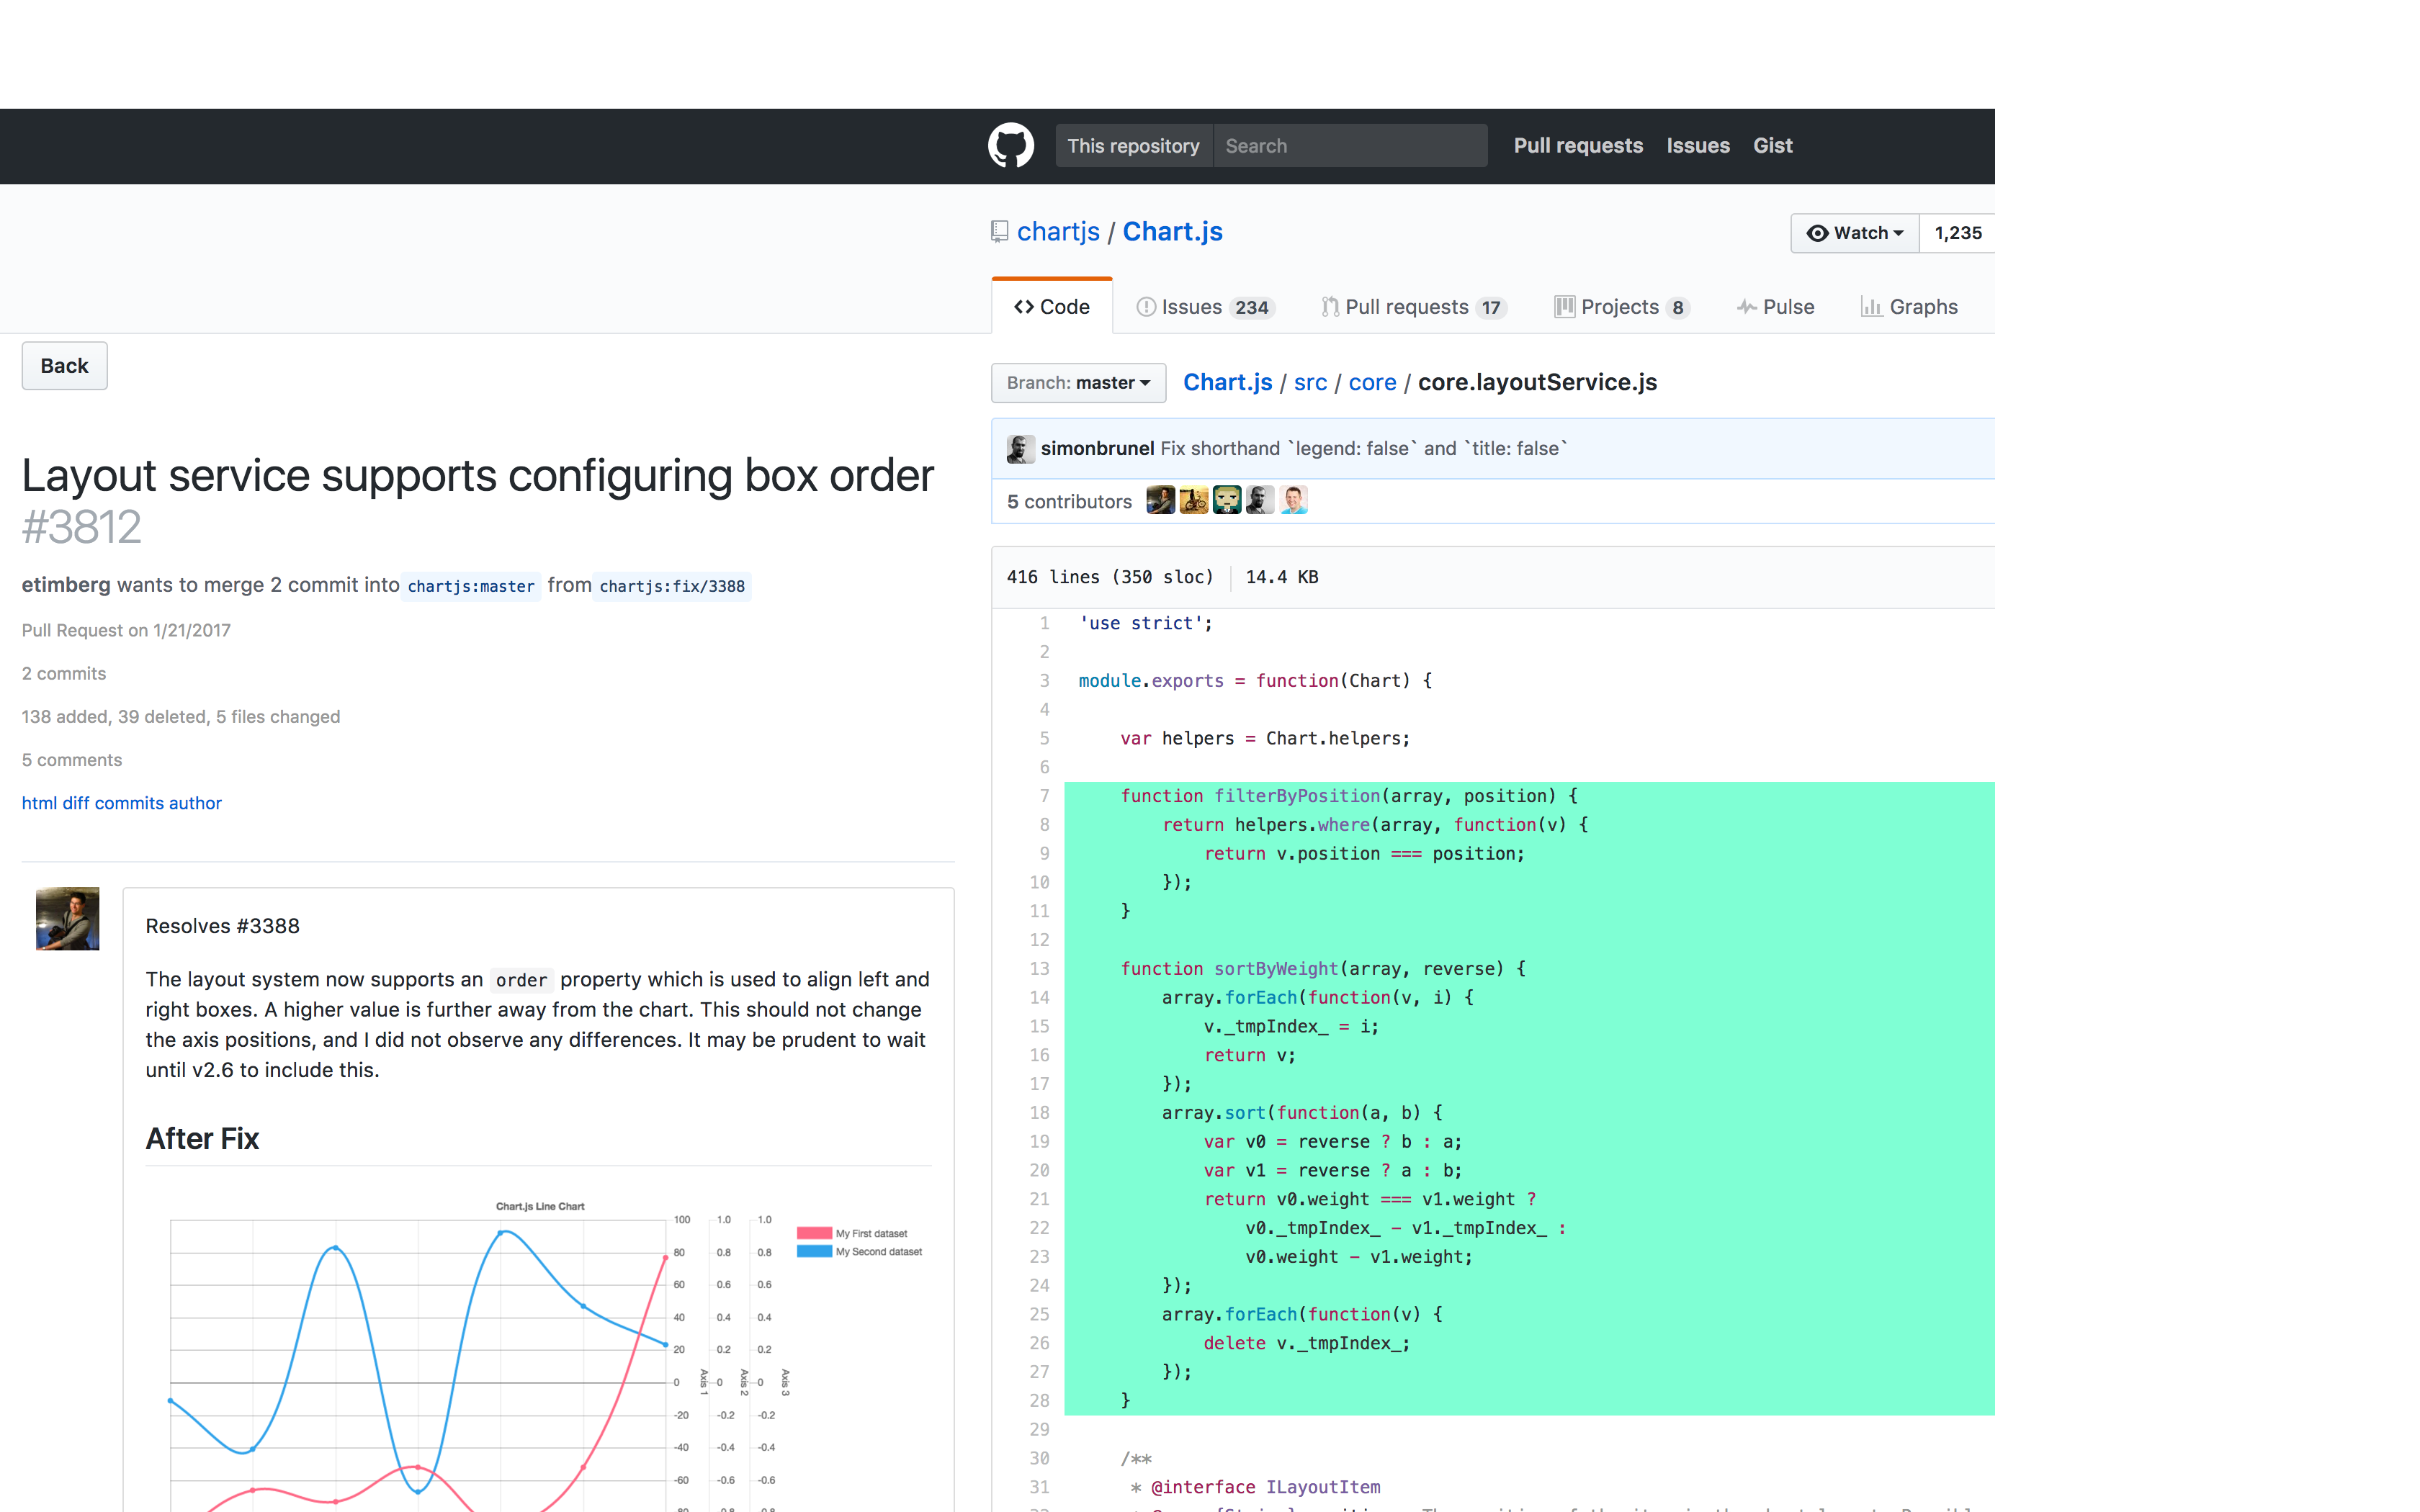
\includegraphics[width=1.2\columnwidth]{interface/top_image.png}
\caption{CodeGlass上でユーザは選択したコード断片に関連する過去のプルリクエストを参照することができる.プルリクエストの説明文に含まれる実装内容や開発背景といった情報は,ユーザのコード理解を支援することができる.}
% \caption{CodeGlass allows users to interactively examine descriptions and comments in pull requests relevant to the chosen portion of code (highlighted in light green). Information in these pull requests can be useful to understand the background of development.}
~\label{fig:top}
\end{figure}




\section{関連研究}

% 効率的なソースコードの理解のためには,実行内容や開発背景といったコードに関連する情報を収集することが重要である~\cite{Program_comprehension_during_software_maintenance_and_evolution}.
% ヒューマン・コンピュータ・インタラクションやソフトウェア工学の研究分野では,コードに関連する情報の検索を様々な側面から支援するための研究が行われてきた.
% 本章では,その中でも特に本研究と深く関係する次の3つの研究領域における先行研究について述べる.

% \shibato{}{日本語でコロンってどう使うんだろうか}

% \begin{itemize}
%   \item コード変更の理解の支援
%   \item ドキュメントの作成と活用の支援
%   \item ソースコード及びプロジェクトの可視化
% \end{itemize}


% Code comprehension involves seeking information to acquire knowledge about code ~\cite{Program_comprehension_during_software_maintenance_and_evolution}.
% Research in HCI and software engineering has explored ways to support various activities around code comprehension.
% We review three major research areas in code comprehension support closely relevant to our work: supporting code change understanding, creating and using documentation, and visualizing code and project.

\subsection{コード変更の理解支援}

GitHubをはじめとする多くのソフトウェア開発管理システムでは,コード差分を記録する事でコード変更の追跡が可能となっている.
加えて,開発管理システムの多くがバージョン管理の機能を提供しており,コード変更の管理やコードレビューのために広く活用されている.
先行研究では,ソフトウェア開発におけるコード変更を理解する事を支援するための様々な手法が調査されてきた.

% Modern project management systems include the diff function by default, and enable code change tracking.
% They also introduce the notion of commits, used for version controls and code reviews.
% These code changes and related descriptions can contain helpful information to understand code.
% Prior research has examined approaches to supporting documentation and comprehension on code changes.

ソースコードの多くの部分に影響を与えるコード変更がバグを含んでいた場合,システムに重大な問題が生じてしまう恐れがある.
Bucknerら~\cite{JRipples}が開発したJRipplesでは,構文解析を行うことにより,コード変更にバグが含まれていた際にソースコードの中で影響を受ける可能性があるクラスをユーザに提示する事ができる.
Zhangら~\cite{Interactive_Code_Review_for_Systematic_Changes}が開発したCRITICSは,与えられたコード変更と類似した過去のコード変更を提示することにより,コード変更にバグが含まれることを防ぐために着目すべき点を開発者がより正確かつ効率的に発見する事が可能となった.
JRipplesやCRITICSがコードレビュアーのコード理解の支援を目的としている一方で,正確なコードレビューを行うためにはコード変更の説明が詳細に記述されている事も重要である.
そこでBuseら~\cite{Automatically_Documenting_Program_Changes}は,コード変更からその説明文を自動生成する手法を実装した.
ユーザ評価の結果,既存のコミットメッセージの89%はBuseらの手法を用いて生成できうる内容である事が分かった.
% 彼らのユーザ評価では,自動生成された説明文は既存のコミットメッセージの89\%を\sakaguchi{代替可能}{わかったのですが1回目は?となってしまいました…(既存のコミットメッセージの89%は彼らの手法を用いて生成できうる内容である?)}である事が分かった.
同様に,Linares-Vasquezら~\cite{ChangeScribe}が開発したChangeScribeもまた,コミットメッセージとして使用可能な説明文をコード変更から自動生成するシステムである.
ChangeScribeには説明文にコード変更の内容だけでなくその背景も含めるために,複数の情報抽出アルゴリズムが実装されている.

% Zhangら~\cite{Interactive_Code_Review_for_Systematic_Changes}はコード変更の理解を支援するCRITICSというシステムを開発した.
% \shibato{CRITICSは与えられたコード変更と類似した過去のコード変更とそのレビューの記録を管理システムから検索する.}{double-check}
% 開発者はその記録を見る事で,コード変更の理解をより正確かつ効率的に行う事ができる.
% Buseら~\cite{Automatically_Documenting_Program_Changes}はコード変更のデータからその説明文を自動生成する手法を実装した.
% 彼らのユーザ評価では,自動生成された説明文は既存のログの89\%を代替可能である事が分かった.
% 同様に, Linares-Vasquezら~\cite{ChangeScribe}が開発したChangeScribeもまた,コミットメッセージとして使用可能な説明文をコード変更から自動生成するシステムである.
% コミットの内容や文脈を説明文に付与するために\masaki{.}{,}ChangeScribe\masaki{は}{には/では}複数の情報抽出アルゴリズムが実装されている.
% しかし,彼らのシステム評価ではユーザの主観的な調査が行われていない.

% Buckner et al.~\cite{JRipples} presented JRipples, a system that helps developers understand how code changes can impact the rest of a project.
% This system shows classes which may have been impacted, and developers can confirm if code changes cause any major issue.
% Zhang et al.'s CRITICS~\cite{Interactive_Code_Review_for_Systematic_Changes} identifies similar code changes to the given diff.
% With the support of CRITICS, developers were able to conduct code review more efficiently and accurately.
% Buse et al.~\cite{Automatically_Documenting_Program_Changes} examined a method to automatically generate user-readable documentation from diff results.
% Their study found that generated descriptions could serve as substitutes in 89\% of log messages.
% Similarly, ChangeScribe by Linares-Vasquez et al.~\cite{ChangeScribe} automatically creates descriptions which can be used as commit messages.
% Their system incorporates different information extraction methods to infer the content and contexts of commits~\cite{Using_stereotypes_to_help_characterize_commits,Automatic_Generation_of_Release_Notes}.
% Their study, however, did not include subjective examinations on generated messages.


本研究の目的は,前述の先行研究とは異なり,コード断片の理解支援である.
コード理解においては,コード変更に付随する説明文が有益である事が既に明らかとなっている~\cite{Commit_2.0, How_Do_Software_Engineers_Understand_Code_Changes}.
本研究はコード断片に関連する過去のコード変更を抽出し,それらに含まれる説明文をユーザに提供する事で,コード断片の理解支援を目指す.

% Our primary focus is to support comprehension on a portion of code using GitHub pull requests.
% Prior work found that descriptions in commits are often useful to understand code changes~\cite{How_Do_Software_Engineers_Understand_Code_Changes}.
% A system like ChangeScribe~\cite{ChangeScribe} aims to support creating descriptions in commits whereas the main objective of this work is to utilize them as an information resource for code comprehension.

\subsection{ドキュメントの作成と活用の支援}
%APIのドキュメントなど,ドキュメンテーションを作ることとそれらを利用することサポートするようなものをここにいれる.

ドキュメントはコード理解における有用な情報源であり,その重要性は広く認知されている.
しかし実際のソフトウェア開発プロジェクトではドキュメントを作成する時間が不足している事が多い\cite{A_Study_of_the_Documentation_Essential_to_Software_Maintenance}.
そこでドキュメントの作成支援や,既存のドキュメントを活用したコード理解の支援に関する研究が広く行われてきた.


% Documentation is another main resource for code comprehension.
% Although the importance of documentation is well known, developers do not spare time and effort to create it in practice~\cite{A_Study_of_the_Documentation_Essential_to_Software_Maintenance}.
% Research has examined various approaches to lowering the burden of creating documentation as well as utilizing information in existing documents.


Sridharaら~\cite{Automatically_Detecting_and_Describing_High_Level_Actions_Within_Methods}はJavaの関数の要約を自動生成するSWUMというシステムを実装した.
SWUMはソースコード全体と関数の構造的関係性を解析する事で,ドキュメントとして使用可能な関数の説明文を自動生成する事ができる.
McBurneyとMcMillan~\cite{Automatic_Documentation_Generation_via_Source_Code_Summarization_of_Method_Context}はSWUMをさらに改良し,与えられた関数のコード内での使用例も追加できるようにした.
これらの手法により,自動生成される説明文に文脈を考慮した情報を追加する事が可能となった.
またStylosら~\cite{Jadeite}は,JavaのAPIのドキュメントが簡単に検索できるようになるJadeiteを開発した.
ユーザはJadeite上でドキュメントにエイリアスとなるクラス名や関数名を追加する事ができる.
このエイリアスは実際のJavaのAPIと紐づいており,ユーザはAPIの名前だけでなくそのエイリアスでもAPIのドキュメントを検索する事ができる.

% Sridhara et al.~\cite{Automatically_Detecting_and_Describing_High_Level_Actions_Within_Methods} developed a technique to automatically generate summary comments for Java methods.
% An algorithm in their system, called SWUM, can capture linguistic and structural relationships of keywords in code as well as count their occurrences.
% This enables rich textual descriptions about code that can be used in documentation.
% McBurney and McMillan~\cite{Automatic_Documentation_Generation_via_Source_Code_Summarization_of_Method_Context} further improved Sirdhara et al.'s approach by incorporating information about how methods are used in other parts of code.
% In this manner, they were able to include context information in auto-generated descriptions.
% Stylos et al.~\cite{Jadeite} presented Jadeite, a system which enables users to collaboratively edit Java API documentation.
% The system lets users annotate documentation with an alias class or method names which they expect to exist.
% These alias names, or placeholders, can be linked to existing APIs, and offer other developers multiple ways to reach to a desired API method.


既存のドキュメントをコード理解のために活用する先行研究も多く存在する.
Stack Overflowの投稿にはAPIの使用方法が記述されている事が多いため,ユーザは独自にドキュメントを作成・管理する事なくAPIの使用方法を参照できる可能性がある.
そこで,Subramanianら~\cite{Live_in_Documentation}はAPIとStack Overflow上の投稿のコード例を紐付けるアルゴリズムを実装した.
またDekelとHerbsleb~\cite{Improving_API_Documentation_Usability_with_Knowledge_Pushing}は,膨大なドキュメントからコード理解において重要な情報を抽出することでコード変更のデバッグの成功率を改善できる事を示した.
さらにTreudeら\cite{Augmenting_API_Documentation}は,教師あり学習を用いてStack Overflowから現在のドキュメントには含まれていない情報を抽出する手法を実装し,教師なし学習を用いた手法と比較してより多くの有用な情報をStack Overflowから抽出できることが明らかとなった.

% Research has also explored systems to encourage \textit{in-situ} use of existing documentation.
% Subramanian et al.~\cite{Live_in_Documentation} developed an algorithm to associate API methods with code examples available in Stack Overflow.
% In this manner, developers can easily access actual examples of API use.
% Dekel and Herbsleb's eMoose~\cite{Improving_API_Documentation_Usability_with_Knowledge_Pushing}, extracts imperative directives from documentation as important descriptions.
% %attempts to solve an issue of an overwhelming amount of descriptions in documentation. Their system 
% A user study found that the presence of eMoose improved the success rate of debugging tasks.
% Treude and Robillard~\cite{Augmenting_API_Documentation} used a supervised approach to extracting unseen information in API documentation from Stack Overflow.
% An evaluation confirmed that their method was able to extract more sentences that are meaningful and do not exist in API documentation than unsupervised approaches.

このように既存の情報源を活用したコード理解の支援に関する研究が広く行われてきたが,情報源としてのGitHubのプルリクエストの有用性はまだ明らかとなっていない.
プルリクエストはGitHubを用いた開発において一般的に使用されており,プルリクエストの説明文はドキュメントとして活用できる可能性がある.
コード理解を支援するための情報源としてのGitHubのプルリクエストの可能性を示すことも本研究の目的の1つである.

% Pull requests are a common practice in GitHub, and their descriptions may serve as documentations.
% This work thus complements the research above by utilizing pull requests as an information resource for code comprehension.

% \subsection{ソースコード及びプロジェクトの可視化}
% %コードやプロジェクトの推移を可視化するようなものをいれる.


% 先行研究では,ソースコードの変更の推移を可視化する手法についても広く調査されている.
% Girbaらによるコード変更可視化システム~\cite{How_developers_drive_software_evolution}は,トラブルの原因となるコードに変更を行った開発者の同定を効率的に支援する.
% Wittenhagenら~\cite{Chronicler}が開発したChroniclerではChroniclerはソースコードの推移を表すツリー状のグラフを通じて,ソースコードの過去の変更をインタラクティブに調査することを可能とする.
% 一方でBragdonら~\cite{Code_Bubbles}は,コードを関数などの意味のある断片に分割し,バブル状にコード断片を可視化する事ができるシステムを開発した.
% この可視化を使用する事でユーザは,ソースコード全体から目的の関数に到達するための時間を短縮する事が可能となる.
% また,McMillanら~\cite{Portfolio:_Finding_Relevant_Functions_and_Their_Usage}は関数の定義と使用箇所を検索し特定するPortfolioというシステムを開発した.
% Portfolioは関数とその呼び出しをネットワーク状に可視化する事ができる.

% % Researchers have also investigated interactive visualization to explore the context and usage of code.
% % Girba et al.~\cite{How_developers_drive_software_evolution} developed Ownership Map visualization which illustrates when and how contributors have engaged in a project.
% % Chronicler~\cite{Chronicler} allows developers to interactively examine the history of source code using Tree Flow visualization.
% % Their user study participants preferred Chronicler to an interface without visualization though quantitative performance metrics did not show significant results.
% % Bragdon et al.~\cite{Code_Bubbles} developed an interface which visualizes code by splitting into meaningful chunks (e.g., functions and methods) and showing them in separate bubble-like windows.
% % Their visualization was helpful to reduce the number of navigations and repeated interactions for examining code.
% % McMillan et al.~\cite{Portfolio:_Finding_Relevant_Functions_and_Their_Usage} presented Portfolio which supports users to find definitions and usage of functions.
% % The system visualizes a network graph in which nodes and edges represent functions and their invocations, respectively.

% ソースコード情報の可視化は本研究の主目的ではないが,上記研究で検討された可視化手法は将来のCodeGlassにおいても適応できる可能性があり,プルリクエストの新しい利用を促すものになりうる.

% These projects suggest that code and project visualization can facilitate comprehension.
% Our work encourages future research on visualization techniques for pull requests which none of the projects above has examined.


\section{インタビュー調査}
% \section{Formative Study}
\label{section:Formative_Study}

\subsection{プログラマの要望調査}

実際のソフトウェア開発でのコード理解における障壁を調査するために,我々はIT企業に所属する5人のプログラマ(PA1--5,全員男性)にインタビューを行った.
実験参加者は全員,ソフトウェア開発プロジェクトにおいてGitHubを日常的に利用していた.
インタビューでは実験参加者がコード理解をどのように行い,その際にどのような障壁が存在するのかを重点的に尋ねた.


% システムのデザインの方向性を決定するために,我々は5人の\shibato{プロのプログラマー}{professional programmer}(PA1--5, all 全員男性)に\shibato{事前インタビュー調査}{formative study}を行なった.
% 実験参加者は全員,仕事において日常的にGitHubを利用している.
% コード理解の重要性は既に広く知られているため,このインタビューは実験参加者がコード理解をどのように行い,その際にどのような障壁が存在するのかを明らかにすることとした.

% To be informed of the interface design, we conducted a formative interview study with five professional programmers (PA1--5, all male).
% All participants regularly used GitHub in their work environments.
% Because it is already well known how important code comprehension is in general, our interview focused on how they normally developed code understanding and what issues they encountered.
% As a result, this formative study revealed the following two findings.

%Our interview study took approximately one hour.
%The participants were offered a compensation of approximately 15 USD in the local currency at the end of the interview.
%As we conducted our interviews in a local language, we translated quotes in English for the following report.


% \begin{figure*}[t]
% \centering
%   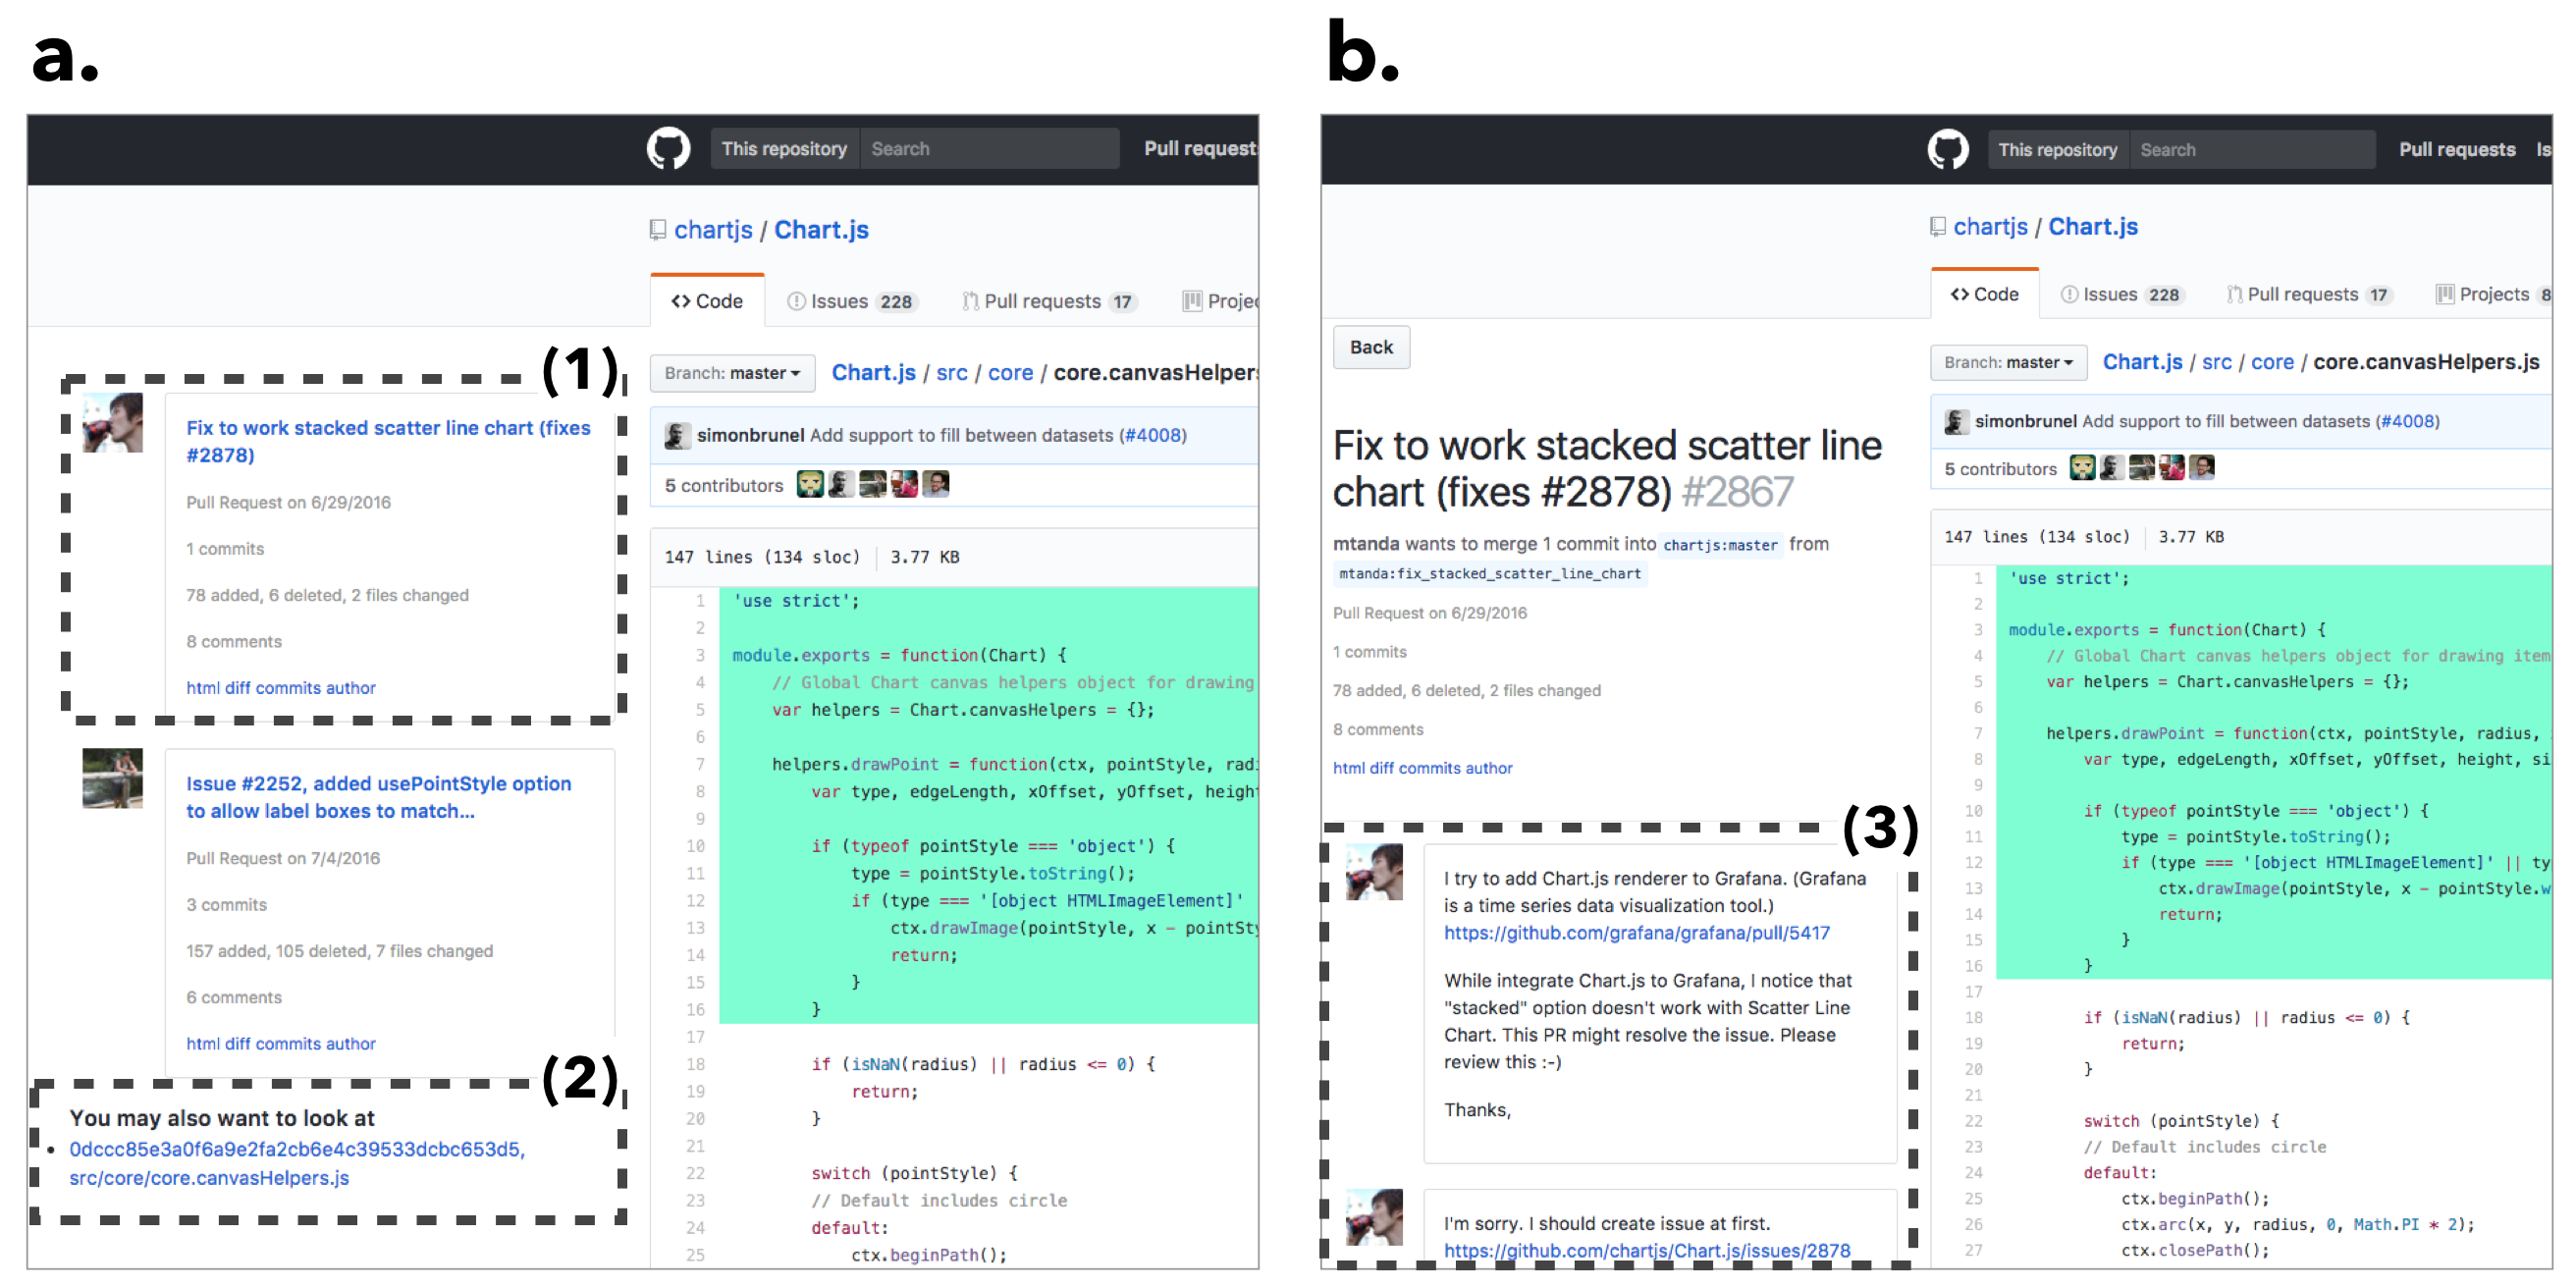
\includegraphics[width=2.0\columnwidth]{interface/CodeGlass.png}
%   \caption{The CodeGlass interface displays a series of pull requests associated with the user-selected code piece (highlighted in light green) in the chronological order. (1) Each pull request is summarized in a separate box. A summary shows the title of a pull request, its ID, and the numbers of commits, lines and files changed, and comments as well as links for additional information. (2) CodeGlass also suggests commits that are not included above but can be relevant if there exists any. When clicking one of them, the user can view the version associated with the selected commit and further investigate how code has been developed. (3) When the user clicks the title, CodeGlass presents review comments in the selected pull request.}~\label{fig:WebInterface}
% \end{figure*}


\subsubsection*{開発背景を理解する難しさ}
% \subsection{Burden for Collecting Development Contexts}

% チーム開発においては,実装やコードレビューのために他の開発者が実装したソースコードを理解する必要がある.
% しかし,他人が書いたコードの理解には大変な労力を要する.
% PA1はコードレビュー時にコード変更を理解することが困難となっていると指摘した.

% In collaborative development, understanding code written by others is crucial.
% However, effort for code comprehension can be substantial. 
% PA1 stated how tedious it can be when he was involved in code review.

% \myquote{(コードレビューにおいて,人のコードを読む事は)まじめにやるとコード書くのと同じくらい時間かかるんですよ}{PA1}
% \myquote{(In code review,) Understanding others' code can be as time-consuming as writing code if you do it seriously.}{PA1}

チーム開発においては,実装やコードレビューのために他の開発者が実装したコードを理解する必要があるが,他人が書いたコードの理解には大変な労力を要する.
また,実際のソフトウェア開発におけるコード理解では,コードの実装内容だけでなく,なぜ実装されたのかという開発背景も把握することが重要である.
%何故なら,実際のソフトウェア開発では厳格な締め切りやビジネス上の理由により,常に最善の実装方法が選択されるとは限らないからである\shibato{}{cite}.
PA1は,コードレビューにおいて背景知識の不足がコード理解における問題の一つであることを以下のように指摘した.
%特にチームの新しい開発メンバーにとってはこの問題は深刻である.

% Code comprehension includes understanding the context of how the code has been developed in addition to what it executes.
% PA1 mentioned a particular issue related to code review caused by the lack of context understanding.
% Such development contexts is important particular for new team members.

\myquote{プロダクトの背景がわからないことが課題となっていて,長く見ている人が初めてそのチーム内でレビューできるようになっていて,まだやっぱり新入りの人がコードレビューできるような状況までドキュメントが整備されていないし,やっぱり背景理解が難しい.}{PA1}

% \myquote{One issue is the lack of background knowledge about the product. It makes only old members able to perform code review. Documentation is not ready for new members, and they cannot perform code review. It is still difficult for them to understanding the background.}{PA1}

% This problem becomes more prominent when new team members were on board.
% P1 mentioned that he frequently observed that new team members struggled on collecting background information.

% % \myquote{やっぱりコードの背景というか,コンテキストがわからないので,そこはなんかわかんないのは当たり前だと思う}{P1}
% \myquote{It is unsurprising that new team members do not understand the project well because they do not know its context or background.}{P1}

% \myquote{どういう背景があってこのコードを実装したのかが書いてあると嬉しい.}{P3}
%\myquote{It would be great if it is clear why this code has been implemented.}{PA3}

% Software documentation is one of the best practices to share knowledge of source code among team developers.
% However, PA5 stated that creating documentation would cause additional overhead in a project, and his team decided not to engage in it.

% % \myquote{チーム内でもドキュメントを作ろうという流れになる事はあります,ありますけど,正直なところあのーそこにさけるパワーは今,ちょっと・・,開発スピードを重視したいので}{P5}
% \myquote{We do have plans to create documentation, but to be honest, we don't have bandwidth for it now. We want to focus on speeding up our development.}{PA5}


\subsubsection*{コード理解のための情報源としてのプルリクエスト}
% \subsection{Pull Requests as an Information Resource}

% Code review was a common activity we observed in our interviews.
% It is one development process where a developer validates code revisions developed by another programmer.
% Bacchelli and Bird~\cite{MotivationOfCodeReview-Bacchelli} reported that while the main motivation for code review was to identify defects, reviewers also expected additional benefits, such as learning alternative solutions or performing knowledge transfer.
% For these multi-faceted benefits, code review becomes an integral part of a modern development process.

% GitHub supports code review through pull requests.
% A pull request includes a description of revisions as well as the actual code changes.
% A reviewer performs merge (or pull in GitHub) when she finds the revisions to be bug-free and legitimate.
% Our participants mentioned that additional effort by developers can greatly facilitate a code review process.
% For instance, a well-written description of a pull request can offer a sufficient amount of information about and reasons for the code changes, supporting reviewers' activities.

%適切にコードレビューを行うためには,開発者がレビュアーにコード変更の内容や開発背景を伝える必要がある.
実験参加者らはコード変更をレビュアーに説明するために,GitHubの機能の一つあるプルリクエストを活用していた.
プルリクエストでは,説明文に目的や内容を記述することで,コード変更をより分かりやすく他の開発者に伝えることが可能となっている.
PA3とPA5は,コードが実装された理由を後から確認するために,開発背景といった情報を含むプルリクエストを参照することがあると指摘した.

% 実験参加者らは,彼らのソフトウェア開発においてGitHubの機能の一つあるプルリクエストを活用していた.
% プルリクエストではコード変更の目的や内容を説明に記述する事が出来る.
% 彼らはプルリクエストの説明文やコメント内にコード理解のための有用な情報が多く存在する事を指摘した.
% 例えばPA3とPA5は,そのコードが実装された理由を理解するためによくプルリクエストを参照していると述べた.


% Our participants regularly used pull requests in their projects as part of a code review process.
% They agreed that comments and logs in pull requests can be useful to obtain information about code. 
% For instance, PA3 and PA5 often referred to past pull requests to understand implementation reasons.

\myquote{それは,実装を見ててこれってどういう意図でこうなってんのとかが,気になった時は,結構プルリクエスト上で議論がなされていることが多いので,それを探しに行くことはあります.}{PA3}
% \myquote{When I have a question about why this implementation was made, I look for pull requests because they often include related discussions.}{PA3}

\myquote{僕はわりと探っちゃうタイプなので,昔どういうことあったんだろうみたいなのは追っちゃう感じですね.}{PA5}
% \myquote{I like digging into code, so I often look for pull requests to see what happened in the past.}{PA5}

% PA1 and PA3 stated that they and their team explicitly described contexts as well as the content of changes.


% % \myquote{重要だと思ってるのは,まあ一個一個何でどういう目的でやるのかっていうのを書くようにしてるんですよね,formatをwhyとwhatを書くようにしている}{P1}
% \myquote{What's important to me is to describe what each change does for what purposes. We have a format (for pull requests) to make sure to write why and what.}{PA1}
% % \myquote{見てもらう人のことは考えて,どういう変更をどういう意図で行ったのかっていうのは,書くようにしている}{P3}
% \myquote{I always think of the reader, and clearly write what changes I have made for what purposes.}{PA3}

% Similar to general code comprehension, understanding development contexts is important for code review.
% P4 mentioned that the problem arises when he asked external developers to perform code review. 

% %\myquote{他のチームにレビューを頼む時に,プロダクトの背景がわからないことが課題となっていて,長く見ている人が初めてそのチーム内でレビューできるようになっていて,まだやっぱり新入りの人がコードレビューできるような状況までドキュメントが整備されていないし,やっぱり背景理解が難しい.}{P4}

% \myquote{When I have to ask someone in another team to review, the problem is that he does not have background knowledge about the project. People cannot do proper reviews until they are in a team for a long time.}{P4}




% \subsection{Summary}
% Our interview study thus highlights the following findings.

% \begin{itemize}
% \setlength{\parskip}{1mm}
% \setlength{\itemsep}{0mm}
% %\item Developers are frequently required to understand codes before performing further actions (e.g., reviewing and making revisions).
% \item Developers desire to obtain relevant information about the portion of code they are investigating for understanding, but they do not always have appropriate support.
% \item Past pull requests can be useful to understand the context or reasons of code changes.
% \end{itemize}

以上より,プルリクエストの説明文にはコード理解において有用な情報が含まれている可能性があり,実際に開発現場で利用されることがあることを確認した.
この発見により,プルリクエストをコード理解に活用するシステムを構築することを考えるに至った.

% These findings led us to a hypothesis that improving accessibility to relevant pull requests would support comprehension of code portions.

\subsection{既存技術の問題点調査}
% \section{Study on Existing Command-based Tools}
% %Our interview with professional programmers revealed that past pull requests can be a useful resource for understanding code.

続いて我々は,既存のツール,特にtig\footnote{\url{https://github.com/jonas/tig}}とrecursive-blame\footnote{\url{https://github.com/scottgonzalez/recursive-blame}}がコード理解の支援においてどのように不十分であるかを調査した.
% 続いて我々は,何故プルリクエストを活用したコード理解を既存のツールでは実現できていないのかを調査することとした.
% 続いて我々は,コード断片の理解を支援でき得る既存のツールの評価を行った.
tigはgit blameのコマンドを再帰的に実行できるコマンドラインインターフェースであり,recursive-blameは特定のキーワードを含む過去のコード変更を抽出することができるコマンドである.
%tigとrecursive-blameの技術的先行調査を行った結果,CodeGlassと異なり,コード断片の追跡を自動で再帰的に行うことができないことが明らかとなった.
%したがって,CodeGlassとtigおよびrecursive-blameを同一の条件下で比較評価を行うことは難しいため,我々は定性的な調査を行うこととした.
本調査ではGitHubのプルリクエストを用いた開発経験のある7人の学生(PB1--7)にインタビューを行った.
インタビューではまずtigまたはrecursive-blameを用いてコード断片の調査を行ってもらい,その後2つのツールに対する使用感を尋ねた.
その結果,既存のツールでは過去のプルリクエストをコード理解のために活用することができない2つの理由が明らかとなった.

% We further examined why existing tools cannot support extraction of past pull requests well.
% Specifically, we looked into tig\footnote{\url{https://github.com/jonas/tig}} and recursive-blame\footnote{\url{https://github.com/scottgonzalez/recursive-blame}}.
% Although we initially considered a comparative study, we found a large discrepancy in backtracking capability between CodeGlass and these tools as the following results suggest.
% We thus concluded that a comparison under fair conditions would be difficult, and decided to conduct a qualitative study instead.



% To understand how these tools would be useful even for novice developers, we recruited seven university students (PC1--7) who had sufficient experience in GitHub and pull-request-based development.
% We asked the participants to find pull requests related to portions of code in Chart.js given by the experimenter using tig and recursive-blame.
% We then conducted a short interview to understand the user experience of these tools.
% As a result, we found two major issues that existing tools cannot address well.

% \subsubsection{Limited commit backtracking capability}
\subsubsection*{コード断片追跡機能の限界}

%PC1 stated that recursive-blame often cannot trace back the history when the specified pattern of code was changed.

%\myquoute{単純に名前が変わったりすると追えないとかがあるから,基本的にある程度あいまい検索ができるといいんだと思う}{PC}

%Tig finds the latest commit and version containing a change on the user-selected line of code using the git-blame command.
%However, it may fail to determine the commit when changes are substantial as P6 stated:

% % \myquote{色々書きかえると結構すぐ追えなくなりますよね}{P6}

% %The tools tested only take constrained input for search (a line of code and a regular expression or keyword in tig and recursive-blame, respectively).
% %This limitation prevented our participants from correctly identifying relevant pull requests.


実験参加者らは,既存のツールではコード断片が削除または移動された際に,開発履歴の情報が抽出できなくなることを指摘した.
これはコード断片が削除または移動された場合,既存のツールでは単にコード断片が存在しないことのみが表示されるからである.
% Our participants pointed out that existing tools cannot clearly inform whether the portion of interest was completely deleted or moved from a different part (e.g., by refactoring).
% This is because the tools only indicate the deletion of such a portion, and additional manual confirmation is necessary.

\myquote{違う名前や使い方が変わったときに,じゃあ何になったんだろうというってのを探すためには,前の名前しか知らないときは自分で探さないといけない.削除なのか,変更なのかわからないのが今のツールではわからない.}{PB4}
% \myquote{For example, when I found revisions on names or usage, I have to eyeball to figure out whether deletion or changes had occurred, which  these tools cannot tell me.}{PC4}


% \subsubsection{Limited interaction}
\subsubsection*{インタラクションの限界}

tigとrecursive-blameでは,追跡するコードの行やキーワードを繰り返し指定することで,関連する過去のプルリクエストを特定することができる.
しかし,プルリクエストを特定した際に提示される情報には,説明文やコメントが含まれていないため,コードの理解につながると限らないことが指摘された.

% Although the two tools can identify past pull requests, their interfaces do not offer an overview of descriptions and comments.
% This diminishes the utility of the tools as code comprehension support.
%Our participants commented that an overview of relevant pull requests would be desirable.

\myquote{全部やった後にさ,descriptionなかったらさ,なんやねんって感じやん.多分descriptionが一番大事だから,はずれだったらすぐ次のを見せてほしい.}{PB2}
% \myquote{I think descriptions are the most important. So I want to have a way to quickly move on to the next if the current pull request isn't useful.}{PC2}

%\myquote{一度にいくつか(プルリクエストを)見られればうれしいかなと思う,まとめて勝手に深追いしてほしい}{PC4}
% \myquote{If I can see multiple pull requests at one time, that would be great. A system should just automatically backtrack for me.}{PC4}

% %P5 wanted a system that simultaneously provides code and description in pull requests.
% % \myquoute{コードと説明文の二つを同時に表示してあげるインタフェースがあると,使いやすいインターフェースかなと思うしとっつきやすいかなと思う}{P5}

tigではコード中の1行を,recursive-blameではキーワードもしくはコード1行のみを検索に利用できるが,コード理解においては複数行の選択が必要であることを指摘していた.

% Tig and recursive-blame take a single line of code and a keyword in the regular expression form for search, respectively.
% Our participants complained that this search method does not fit to their expected use cases, and the tools should support selection of multiple lines or code pieces.

\myquote{コード読んでて,この行だけわかんないってなることはないから.}{PB1}
% \myquote{It's unlikely that I do not understand only this particular line when I read code.}{PC1}

\myquote{このifの中みたいな,意味のある単位で見たい.ifの行自体は別にそれほど興味ないし中身が大事かな,みたいな.}{PB5}
% \myquote{I want to look into a meaningful chunk, such as code inside this if block. I am not really interested in the line of the if statement itself.}{PC5}

% %\subsubsection{Limited search capability}
% % \myquoute{キーワードで検索は面倒というか,自分が思ったところを検索出来ているのか不安.どこが引っかかるか直感的じゃないから,tigのほうがいいかも}{P3}

\subsection{まとめ}

% Our literature survey identified the following five information categories developers seek in code comprehension:
我々が行った関連研究の調査では,コード理解に重要な情報は以下の5つに大別されることがわかった.



\begin{itemize}
\setlength{\itemsep}{0cm}
%\setlength{\leftskip}{-3mm}
\item \textbf{Execution}: そのコードが何を実行するのか~\cite{Information_Needs_in_Collocated_Software_Development_Teams}.
\item \textbf{Rationale}: 何故そのコードが実装されたのか~\cite{Information_Needs_in_Collocated_Software_Development_Teams}.
\item \textbf{History}: そのコードがどう変更されてきたのか~\cite{Chronicler}.
\item \textbf{Contributor}: 誰がそのコードの実装に関わったのか~\cite{Who_can_help_me_with_this_source_code_change}.
\item \textbf{Usage}: そのコードがどこでどう使用されるのか~\cite{Six_Learning_Barriers_in_End_User_Programming_Systems}.
\end{itemize}

% \begin{itemize}
% \setlength{\itemsep}{0cm}
% \setlength{\leftskip}{-3mm}
% \item \textbf{Execution}: What the given code piece executes~\cite{Information_Needs_in_Collocated_Software_Development_Teams}.
% \item \textbf{Rationale}: Why the given code piece is implemented in the way it is~\cite{Information_Needs_in_Collocated_Software_Development_Teams}.
% \item \textbf{History}: How the given code piece has been evolved~\cite{Chronicler}.
% \item \textbf{Contributor}: Who was involved in the implementation of the given code piece~\cite{Who_can_help_me_with_this_source_code_change}.
% \item \textbf{Usage}: Where and how the given code piece is used in a project~\cite{Six_Learning_Barriers_in_End_User_Programming_Systems}.
% \end{itemize}

我々のインタビュー調査により,プログラマが特にコード変更に関する詳細な説明と開発背景の知識をプルリクエストに求めていること,さらに既存のツールではそれが十分に支援されないことが明らかとなった.
したがって,我々が構築するシステムにおいては特にExecutionとRationaleに関する情報収集を支援すべきであると考えた.











\section{CodeGlassインターフェース}

\begin{figure*}[t]
\centering
\begin{minipage}{0.49\textwidth}
    \subfloat[関連するプルリクエストの一覧画面.]
    {
        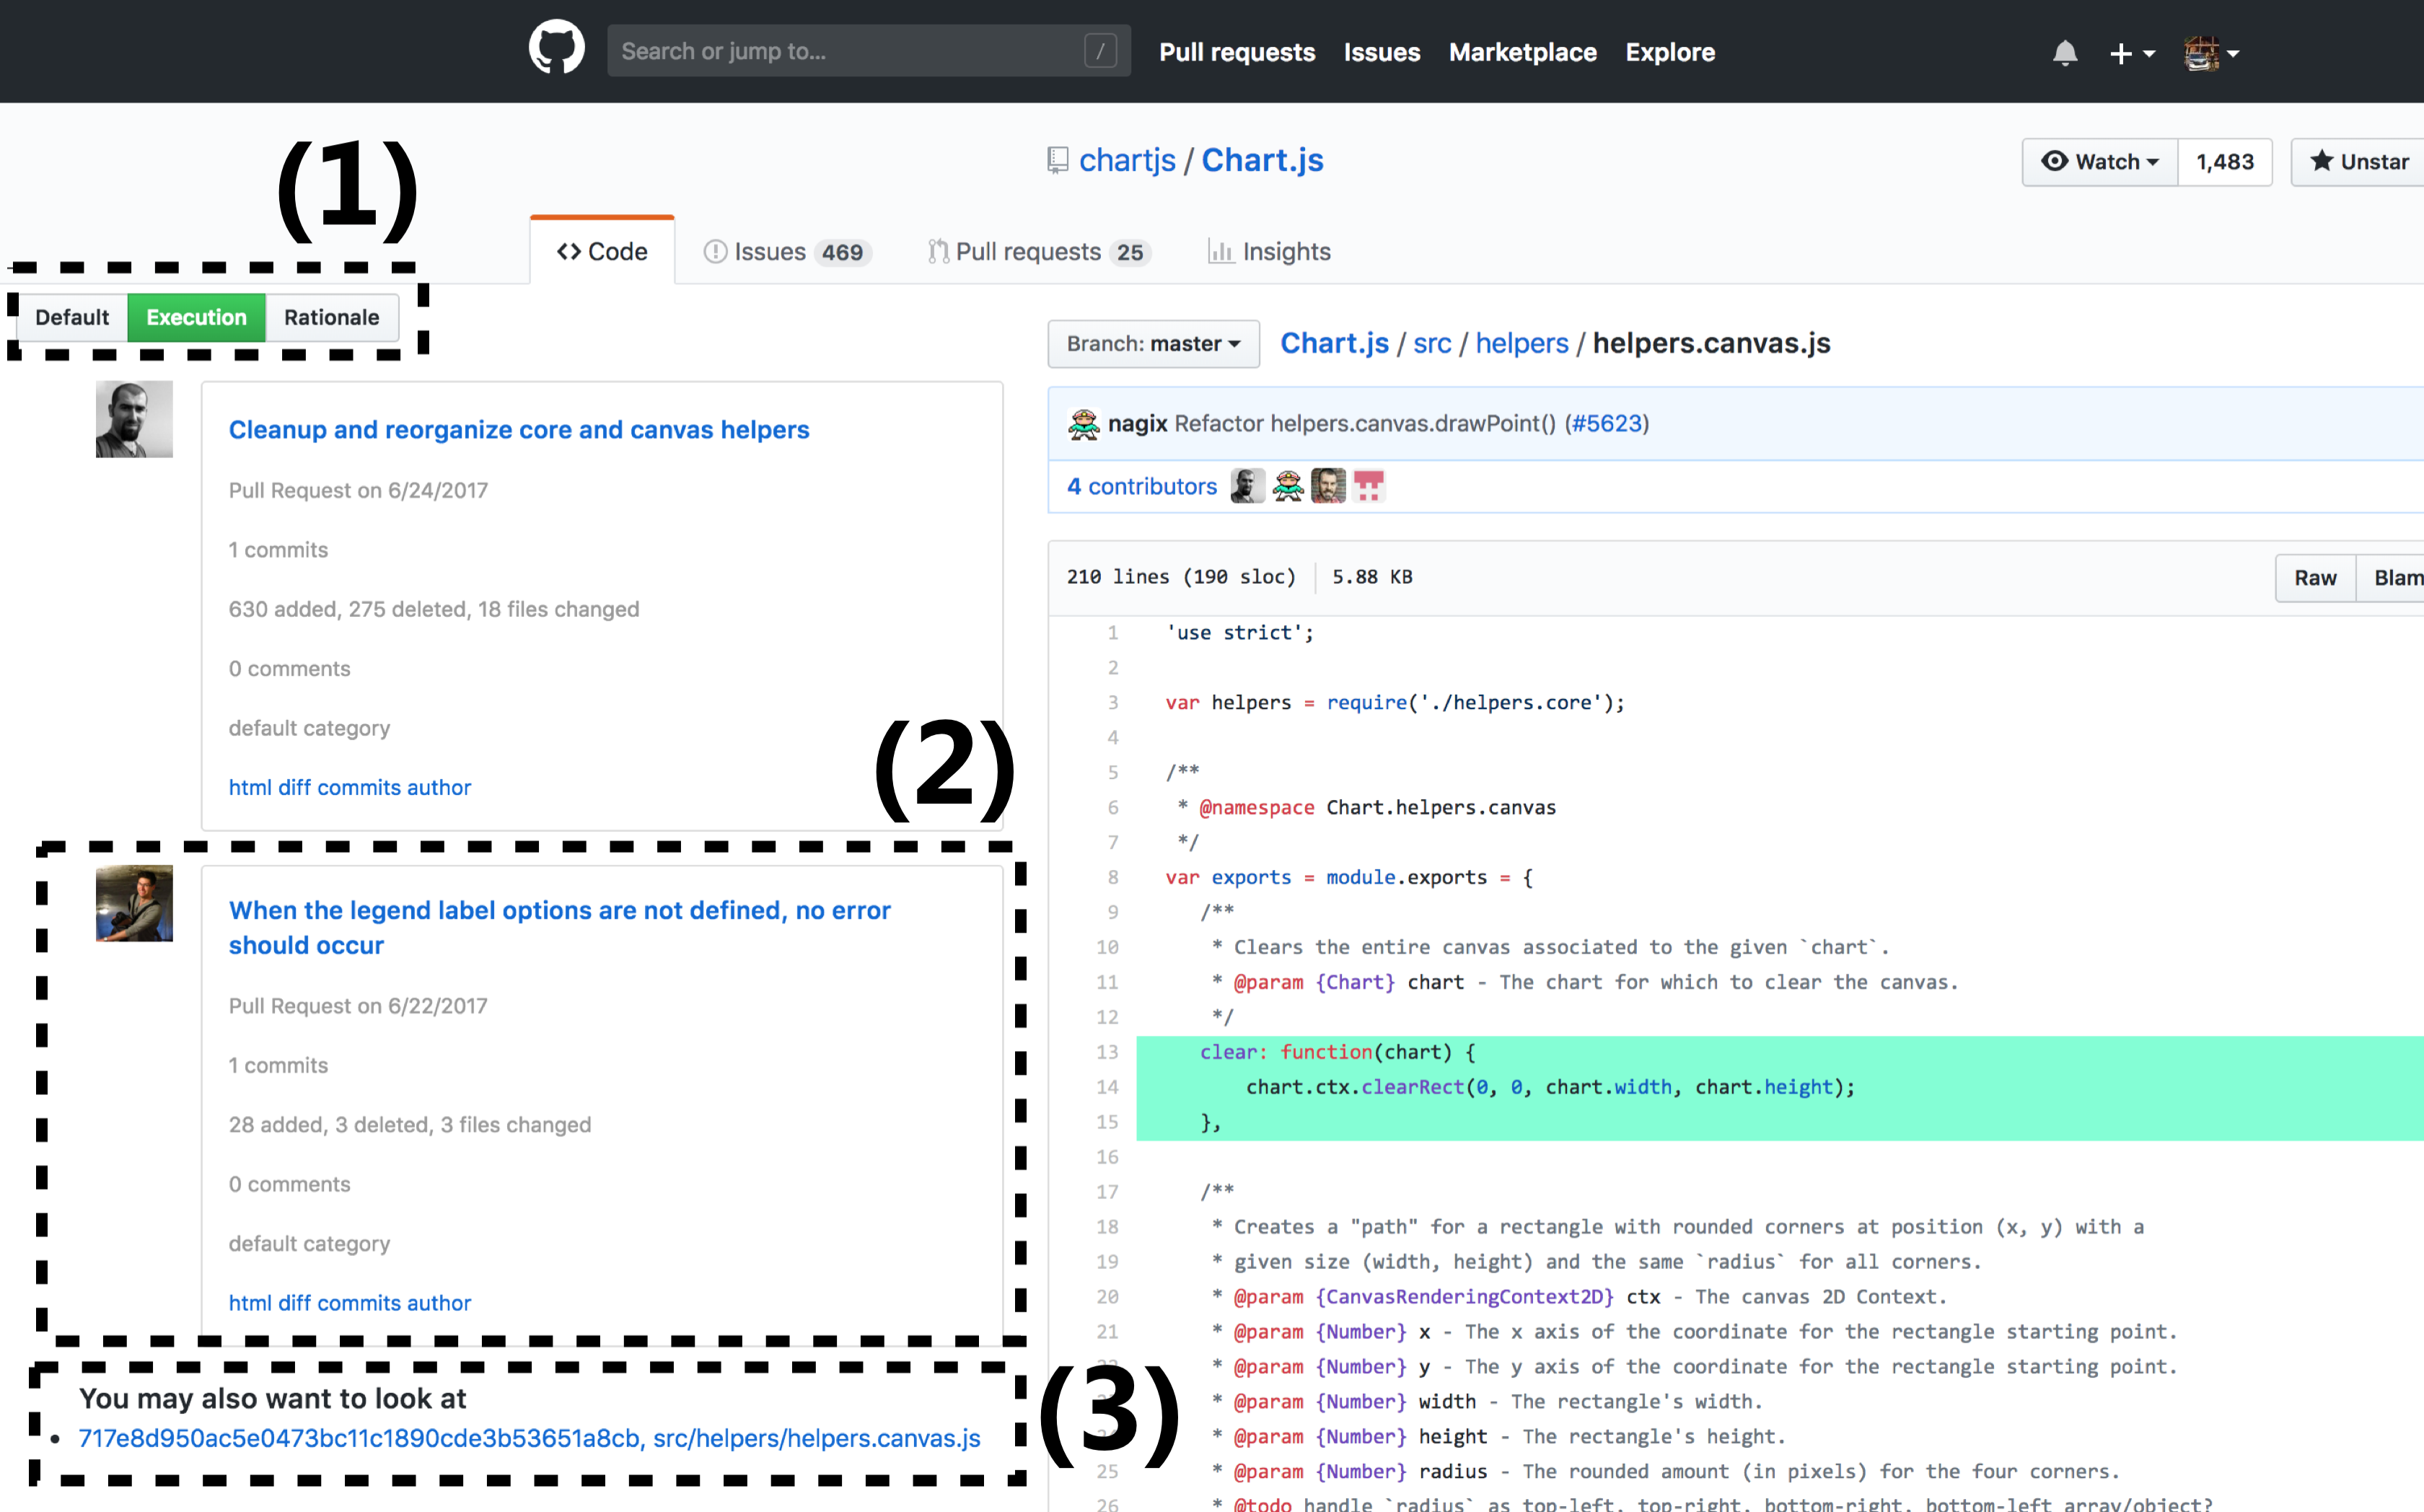
\includegraphics[width=0.95\hsize]{interface/interface1.png}
        \label{fig:interface1}
    }    
\end{minipage}
% \par\hspace{.005\linewidth} 
\begin{minipage}{0.49\textwidth}
    
    \subfloat[プルリクエストの詳細画面.]
    {
        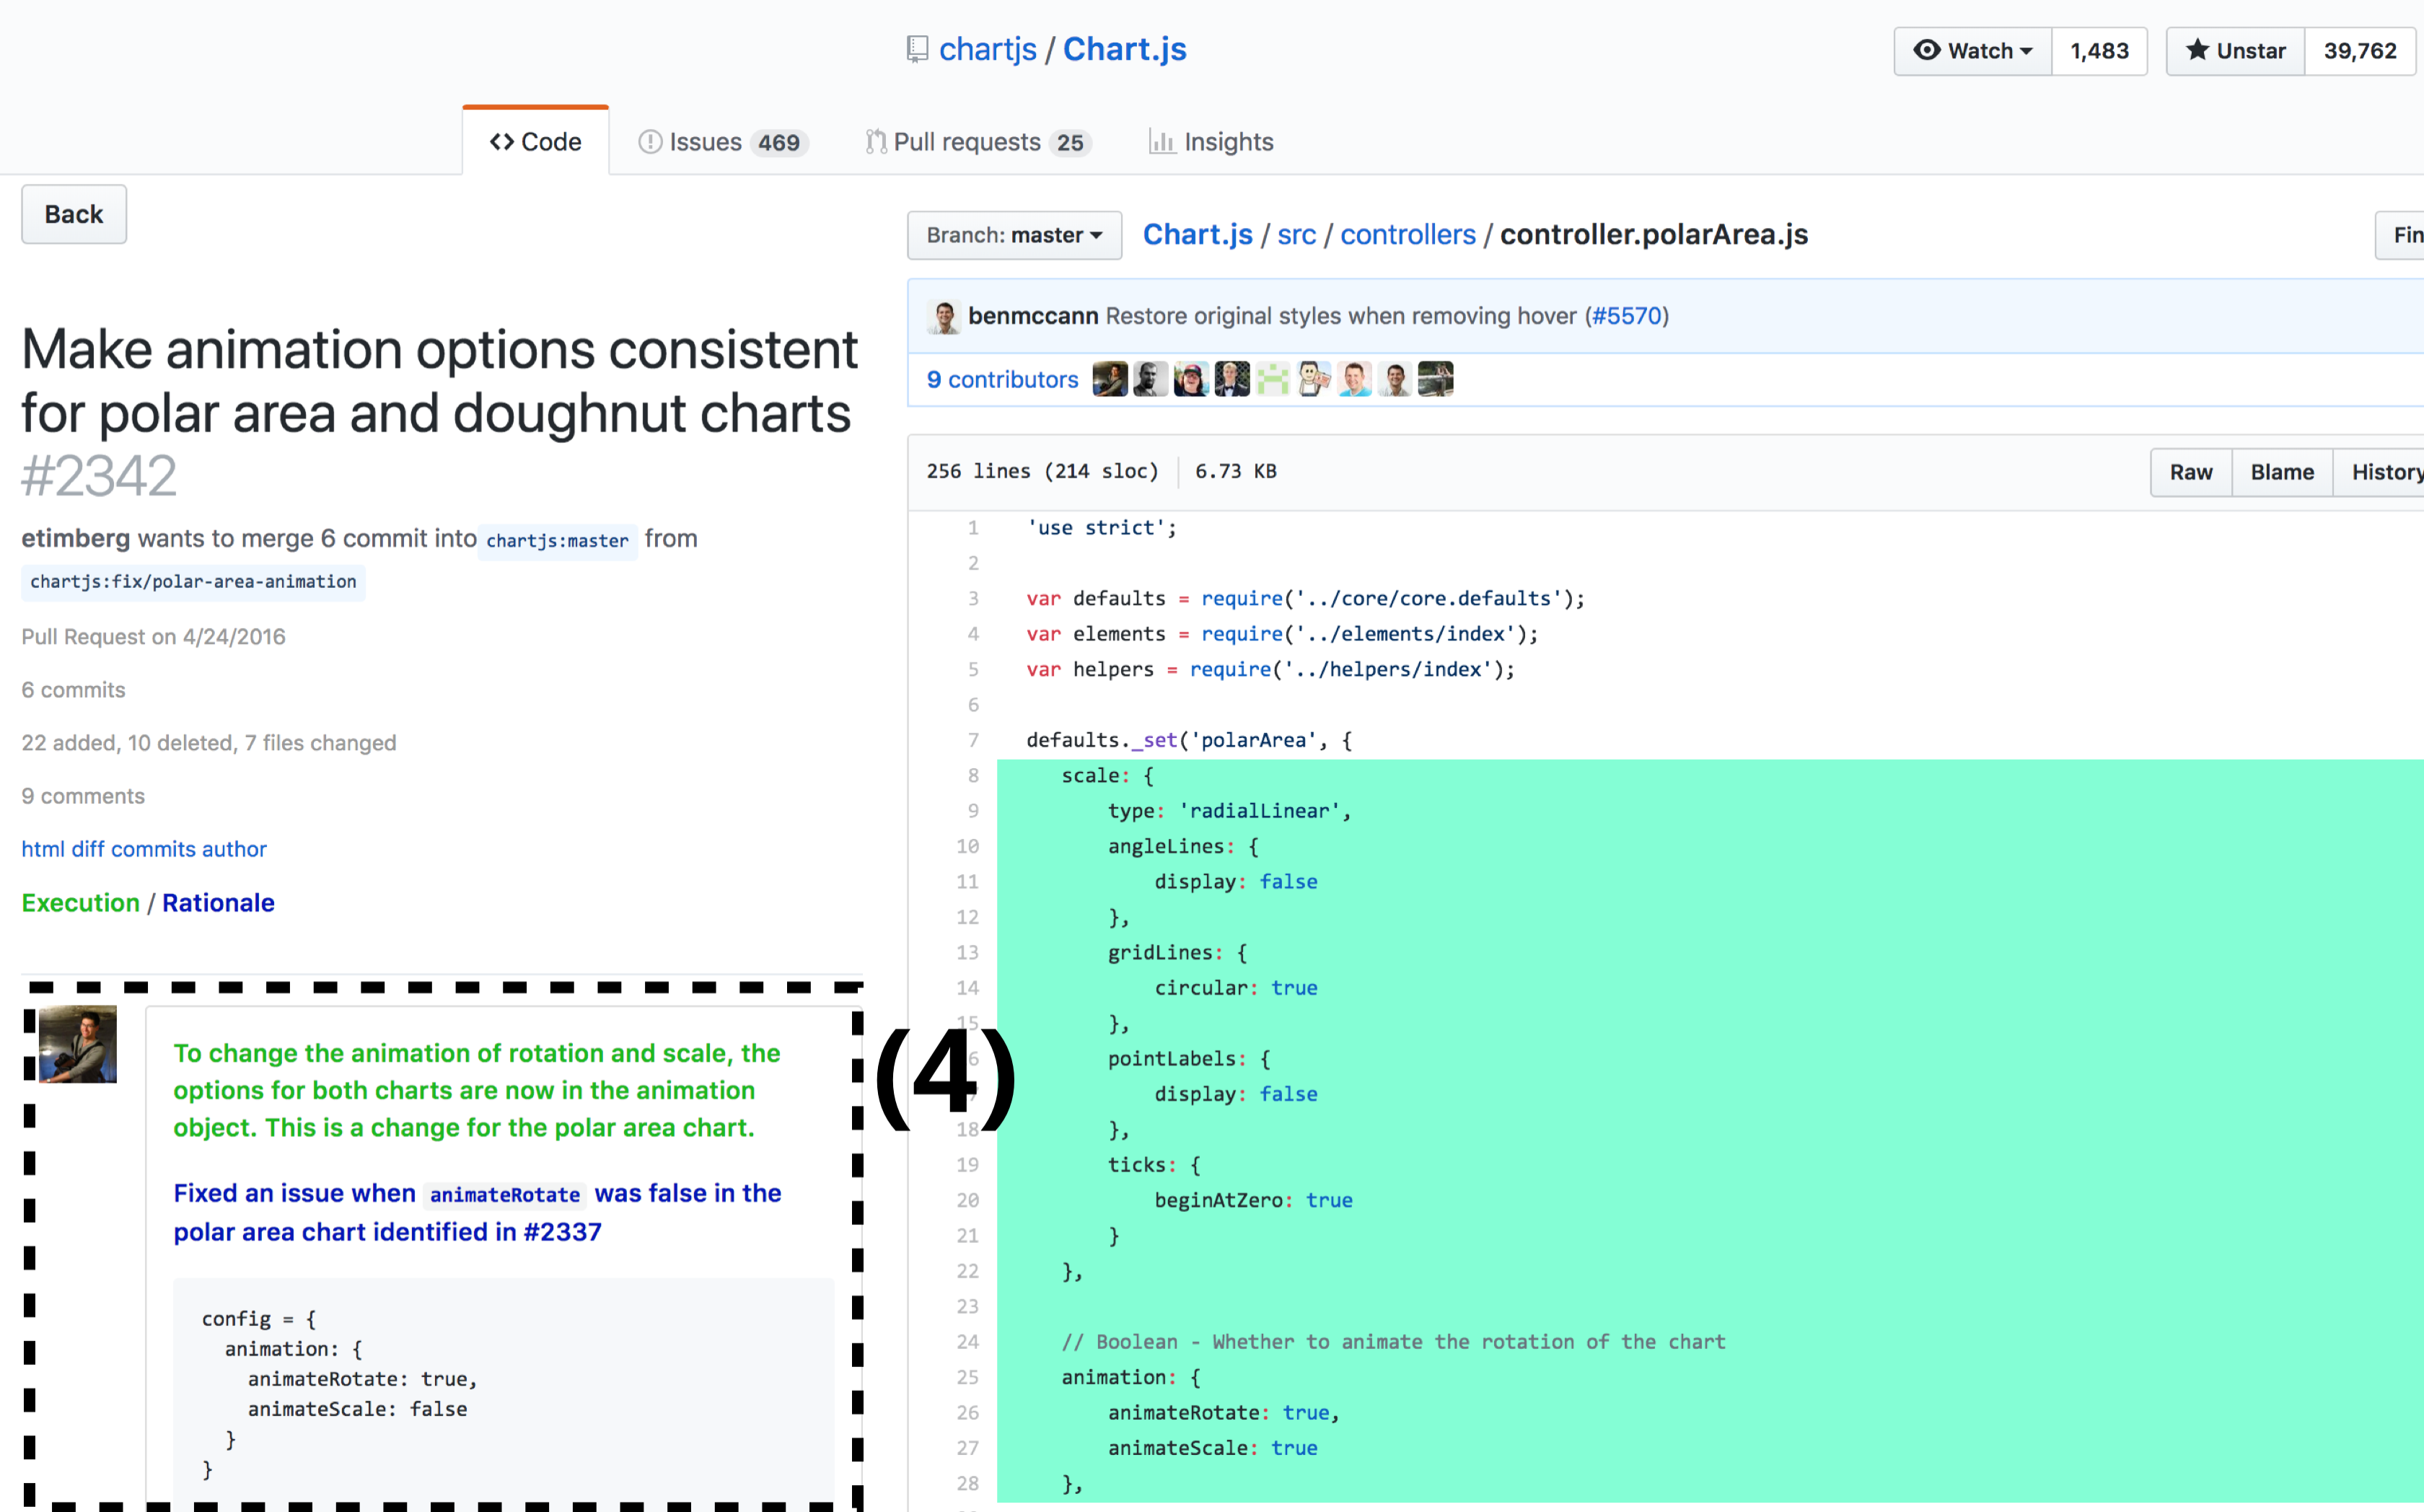
\includegraphics[width=0.95\hsize]{interface/interface2.png}
        \label{fig:interface2}
    }
    
\end{minipage}
	\caption{CodeGlassのインターフェースは,ユーザが選択したコード断片(緑にハイライトされたコード)に関連する過去のプルリクエストの一覧を表示する.抽出されたプルリクエストの表示順は,時系列順,実装内容(Execution)に関する情報が多い順,開発背景(Rationale)に関する情報が多い順に並べることできる~(1).各プルリクエストにはタイトル,コミット数,コードの追加および削除行数,コメント数,そして関連する各ウェブページへのリンクが表示される~(2).さらに,選択されたコード断片と一致する可能性があるコード断片が過去のバージョンの1つで複数ある場合,そのバージョンにおけるソースコードへのリンクが表示される~(3).プルリクエストのタイトルをクリックすると,その詳細情報を確認できる.詳細画面では,プルリクエストの情報に加えて,レビューコメントも表示される.さらに,Executionに分類される文章は緑色で,Rationaleに分類される文章は青色で表示される~(4).}
    \label{fig:WebInterface}
\end{figure*}


CodeGlassはGitHubのプルリクエストを用いてコード断片の理解を支援するインタラクティブなツールである.
本研究におけるコード断片は,ソースコード中の一部の連続したコードである,と定義する.
即ち,コード断片は一行のコードにも,関数やクラス,あるいはファイル全体のコードにもなり得る.
CodeGlassはユーザが選択したコード断片に関連する過去のプルリクエストを抽出し,インターフェースを通じてユーザに提供する.


% We develop an interactive piece-level code examination tool, called CodeGlass.
% The definition of a code piece in this work is consecutive lines in code.
% It can be a single line, function, class or an entire file of code.
% CodeGlass extracts the revision history on the code piece selected by the user.
% Its interface then provides an overview of past pull requests associated with the selected code piece which contain descriptions, commits, and review comments.


図~\ref{fig:WebInterface}にCodeGlassのインターフェースを示す.
ユーザはマウスドラッグでコード断片を指定する(緑でハイライト)事で,関連する過去のプルリクエストやコミットを確認できる(図~\ref{fig:interface1}).
図~\ref{fig:interface1}~(1)に示すボタンから,関連する過去のプルリクエストの表示順を時系列順,実装内容(Execution)に関する情報が多い順,開発背景(Rationale)に関する情報が多い順に並び替えることができる.
これにより,どのように開発が進められてきたか(History)という情報に加えて,実装内容や開発背景を含むと考えられるプルリクエストを強調して提示することも可能となっている.

それぞれのプルリクエストには,タイトルやプルリクエストのID,含まれるコミット数,コードの変更行数,そしてコメント数が表示されている.
また,GitHub上でのプルリクエストや,コード差分,レビューコメント,そしてプルリクエスト作成者へのウェブページへのリンクも示されている.
加えて,図~\ref{fig:interface1}~(3)に示すように,選択されたコード断片と一致する可能性があるコード断片が過去のバージョンの1つで複数ある場合,そのコミットへのリンクも表示する.
ユーザがプルリクエストのタイトルをクリックすると,CodeGlassはその詳細を表示する(図~\ref{fig:interface2}).
詳細画面では,プルリクエストの基本的な情報に加えてレビューコメントも表示される.
また,図~\ref{fig:interface2}~(4)に示すように,プルリクエストの説明文中で実装内容や開発背景に関する情報であると推定された箇所は,色付きの文字で強調される.

% GitHub displays a source code in a file in the red frame in Figure~\ref{fig:WebInterface}.
% CodeGlass provides ``Fetch'' button~(i.e., blue frame in Fig.~\ref{fig:WebInterface}) and a feature that the user can select codes by pointer~(i.e., green frame in Fig.~\ref{fig:WebInterface}).
% Figure~\ref{fig:WebInterface} shows the CodeGlass interface.
% The user specifies a code piece to read descriptions and review comments of past pull requests by a mouse drag~(highlighted in light green in Figure~\ref{fig:WebInterface}).
% CodeGlass displays a series of relevant pull requests in the chronological order as shown in Figure~\ref{fig:WebInterface}a.
% Each pull request is summarized in a separate box ((1) in Figure~\ref{fig:WebInterface}a).
% Each summary includes the title of a pull request, its ID, and the numbers of commits, lines and files changed, and comments.
% It also contains links to the original pull request page, the diff summary, review comments, and the author's page to allow the user to further investigate details.
% In addition, CodeGlass suggests other potentially-relevant commits if there exists any ((2) in Figure~\ref{fig:WebInterface}a).
% When clicking one of them, the user can view the version associated with the selected commit and further investigate how code has been developed.
% When the user clicks the title of a pull request summary, CodeGlass presents its review comments ((3) in Figure~\ref{fig:WebInterface}b).

CodeGlassにおいてユーザは,クラスや関数といった単位に縛られる事なく自由にコード断片を選択し,関連する過去のプルリクエストを調べる事ができる.
特にユーザが大きなクラスや関数のコードを調査する際には,自由にコードを分割して調べる事ができるため有用であると考える.
CodeGlassはプログラミング言語に依存する事なく動作するため,GitHub上の全てのオープンなリポジトリに対して,CodeGlassのサーバにリポジトリをクローンする事で利用可能となっている.
アクセス制限などを設定する事で,技術的にはプライベートリポジトリにも対応する事ができる.


% CodeGlass allows developers to examine past pull requests and commits on any line of code, not limited to meaningful chunks (e.g., classes or functions).
% This capability is useful when developers need to investigate large classes and functions because they can have freedom to break down into smaller portions for their examination.

% 現在のCodeGlassのプロトタイプはサーバとインターフェースの二つに分けて実装されている.
% インターフェースはGoogle Chromeの拡張機能として開発されている.
% サーバはインターフェースからリポジトリ名やファイル名,選択されたコード断片の位置を受け取り,それらに関連する過去のプルリクエストをインターフェースに返す仕組みとなっている.

% CodeGlassはプログラミング言語に依存する事なく動作するため,GitHub上の全てのオープンなリポジトリに対して,CodeGlassのサーバにリポジトリをクローンする事で動作する事が可能となっている.
% アクセス制限などを設定する事で,技術的にはプライベートリポジトリにも対応する事が出来る.


% The current CodeGlass system takes a server-client implementation.
% The CodeGlass interface is implemented as a Google Chrome extension.
% The server accepts information necessary for search (e.g., the repository name, file name, and line numbers) upon user's selection of a code piece, and returns relevant pull request data.

%Our current prototype would function for any public repository on GitHub because the backend algorithm is language-agnostic as we explain later.
%With proper permission settings, CodeGlass would be available even for private repositories.
% There are 57 million active repositories as of April 2017\footnote{\url{https://github.com/blog/2345-celebrating-nine-years-of-\\github-with-an-anniversary-sale}}.










\section{実装内容と開発背景を含む説明文の抽出手法}


\ref{section:Formative_Study}章にて述べたプログラマを対象としたインタビューにより,コード断片の理解においてプルリクエストに含まれる情報が有用であることが示唆された.
また,コード断片を理解する上で,そのコード断片が何を実行するかという実装内容だけでなく,開発背景も理解することが重要であることが明らかとなった.
しかし既存のシステムでは,コード変更の説明文に含まれる情報を,実装内容や開発背景といった情報に分類することは行われていない.
そこで我々は,プルリクエストの説明文内の文章の中から,関連するコード変更の実装方法と関連するコード変更の実装理由を抽出するための分類器を実装した.


\subsection{データセットの構築}

% \shibato{}{ExecutionとRationaleの説明が必要?}

%プルリクエストの説明文に含まれる文章をExecutionおよびRationaleに分類するためには,それらのカテゴリがラベルづけされた文章のデータセットを構築する必要がある.
%そこで我々は,GitHubのリポジトリに登録されているプルリクエストのテンプレートを活用することとした.
開発者が実装内容や開発背景といった重要な情報を漏れなくプルリクエストに記述する事を促すために,GitHubのリポジトリにはマークダウンで書かれたプルリクエストのテンプレートを登録することができる~\footnote{\url{https://help.github.com/articles/creating-a-pull-request-template-for-your-repository}}.
テンプレートに沿ってプルリクエストの説明文を記述することで,他の開発者がコード変更を理解するために必要な情報を網羅したプルリクエストを作成することができる.
テンプレート内のヘッダーには,実装内容(Execution)に該当するヘッダー(``Implementation Details''など)や,開発背景(Rationale)に該当するヘッダー(``Motivation and Context''など)などが多く採用されている.
そのようなヘッダーの下に記述されている文章を抽出することで,分類器の学習に必要なラベルづけされたデータセットを構築することとした.

以上のようなデータをGitHubから収集するために,我々は次の条件を満たすリポジトリに存在するプルリクエストのデータを抽出した.

\begin{description}
\item[条件1] リポジトリのスター数が100以上であること.
\item[条件2] プルリクエストのテンプレートがリポジトリに登録されており, Executionに関係する節かRationaleに関係する節がテンプレート内に存在すること.
\end{description}

条件1はリポジトリの開発者数の目安として掲げたものである.
スター数が大きいものほどGitHub上での開発が盛んであり,条件2を満たすプルリクエストを多く取得できるだろうと考えた.
また,条件2に適応することで,前述のようにラベルづけされたデータを収集することができる.

GitHubから条件1と条件2を満たすデータを収集した結果,26のリポジトリと4061件のプルリクエストのデータを集めることができた.
その26のリポジトリに登録されているプルリクエストのテンプレートについて,著者の2人がExecutionまたはRationaleに該当するヘッダーを手動で抽出した.
そして,それらのヘッダーの下に存在する文章を抽出することにより,Executionの文章を3141件,Rationaleの文章を3451件を得た.
さらに,抽出した文章内に含まれるマークダウン表記と絵文字を削除する事で,分類器の学習用のデータセットを構築した.


% GitHub上のリポジトリの内,以下の条件を満たすものから PR と Issue を取得し,説明文の中から上述の Why と How に関する文章を抽出することで学習用のデータセットを作成した.
% \begin{description}
% \item[条件1] リポジトリのスター数が100以上であること.
% \item[条件2] プルリクエストのテンプレートが存在し, Whyに関係する節かHowに関係する節がテンプレート内に存在すること.
% \end{description}

% 条件1はリポジトリの開発者数の目安として掲げたものである.
% スター数が大きいものほどGitHub上での開発が盛んであり,条件2を満たすプルリクエストを多く取得できるだろうと考えた.
% 条件2はプルリクエストの説明文からWhyまたはHowに該当する文章を抽出するための条件である.
% 開発者が開発目的や実装方法といった重要な情報を漏れなくプルリクエストに記述する事を支援するために,GitHubのリポジトリではマークダウンで書かれたプルリクエストのテンプレートを登録することができる~\footnote{\url{https://help.github.com/articles/creating-a-pull-request-template-for-your-repository}}.
% 開発者はテンプレートのヘッダーで指定された内容をプルリクエストの説明文に書く事で,他の開発者がコード変更を理解するために必要な情報を網羅したプルリクエストを簡単に作成できるようになる.
% 我々は収集したプルリクエストのテンプレートから,Whyに該当するヘッダー(``Motivation and Context''など)とHowに該当するヘッダー(``Implementation Details''など)を指定した.
% そして,それらのヘッダーの下に記述されている文章を,WhyおよびHowを意味する文章として抽出し,分類器の学習用のデータセットとした.

% 我々は条件1および条件2を満たす 26 のレポジトリから,4061件のプルリクエストをGitHubから収集した.
% これらの説明文の中から,Why に関係する文章を3451件,Howに関係する文章を3141件抽出した.
% そして,抽出した文章内に含まれるマークダウン表記,絵文字,urlを削除する事で,分類器の学習用のデータセットを構築した.


% \begin{table}[t]
%     \centering
%      \caption{SVMの結果}
%     \label{table:svm}
%     \begin{tabular}{c | c} \Hline
%      特徴量 &F値 \\ \hline \hline
%      bag-of-words & 0.64 \\
%      tf-idf & 0.68 \\
%      word2vec & 0.72 \\
%      word2vec+tf-idf & 0.73 \\
%     \end{tabular}
% \end{table}


\subsection{分類器の実装と評価}

分類器の実装にはサポートベクターマシンを用いた.
学習に必要な特徴量は,文章の分類において一般的に使用されているbag-of-words, tf-idf,word2vecを用いた~\cite{pmlr-v32-le14}.
さらに,tf-idfとword2vecが抽出する情報が互いに補完的な役割を果たすことが報告されているため~\cite{SVM-word2vec-tfidf},本研究においてもword2vecをtf-idfにより重み付けした特徴量(word2vec+tf-idf)も利用した.
それぞれの特徴量を用いて分類器を学習し,10分割交差検証法により分類器の精度を検証した結果,bag-of-wordsを用いた時のF値の平均が0.64,tf-idfを用いた時のF値の平均が0.68,word2vecを用いた時のF値の平均が0.72,word2vec+tf-idfを用いた時のF値の平均が0.73であった.
以上よりword2vec+tf-idfを用いた時が最も精度が高かったため,word2vec+tf-idfを用いて学習を行った分類器をCodeGlass上に実装した.

% \subsubsection{分類器によるCodeGlassの機能}


% 学習した分類器を用いることで,CodeGlassはユーザが選択したコード断片に関連するプルリクエストを,Executionの情報の量が多い順,およびRationaleの情報の量が多い順に並び替えることができる.
% ただし情報の量は,プルリクエスト内の説明文を分割し生成された各文章に対する,ExecutionまたはRationaleへの分類確率の和と定義した.
% プルリクエストの説明文の分割方法は,説明文にマークダウンが使用されていた場合,ヘッダーを区切りとして分割した.
% また,マークダウンが使用されていない説明文は,空行を区切りとして分割される.
% そして,分割された文章ごとにExecutionおよびRationaleへの分類確率を計算し,それらの和を各プルリクエストに含まれるExecutionおよびRationaleに関する情報の量とする.
% 図~\ref{fig:interface1}~(1)に示すように,CodeGlassは計算した情報の量を用いてプルリクエストを並び替えることができる.
% これによりユーザは,選択したコード断片の調査目的に合わせて,プルリクエストの表示順序を変更することができる.

% 各プルリクエストに含まれるExecutionおよびRationaleの情報の量を計算するために,CodeGlassはまずプルリクエストの説明文を分割する.
% 説明文にマークダウンが使用されていた場合,ヘッダーを区切りとして分割される.
% マークダウンが使用されていない説明文は,空行を区切りとして分割される.

図~\ref{fig:interface1}~(1)に示すボタンから,ユーザはプルリクエストの表示順を時系列順,Executionに関する情報が多い順,Rationaleに関する情報が多い順に並び替えることができる.
さらにプルリクエストの詳細画面では,ExecutionおよびRationaleに80\%以上の確率で分類されると推定された文章がハイライトされる.
図~\ref{fig:interface2}~(4)に示すように,Executionに分類される文章は緑色の,Rationaleに分類される文章は青色の文字で表示することで,ユーザの情報収集を支援することが可能となっている.




% \section{\shibato{コード断片追跡アルゴリズムの改良}{}}


\section{コード断片追跡アルゴリズムの改良}

\label{section:Piece_level_Diff_Backtrack_Algorithm}

\subsection{LHDiffの改良方法}
CodeGlassのサーバは,ユーザが選択したコード断片に関連する過去のコミットを抽出する必要がある.
gitのコマンドであるblameを使う事で,コード断片を最後に変更したコミットを特定する事ができる.
しかし,gitのコマンドではコード断片が過去のバージョンにおけるソースコードのどこに存在するのかを知る事ができない.
したがって,ユーザが選択したコード断片に関連する過去のコミットを最新のものだけでなく全て抽出するためには,選択されたコード断片が過去のバージョンにおいてどこに存在するのかを特定する必要がある.
%以上の手法を実装するために,我々はサーバ上のアルゴリズムについて次の3つの要件を設けた.


% The CodeGlass server system needs to obtain commits that involve changes on the code piece selected by the user.
% Such an algorithm needs to locate the portion in a past commit which best matches with the given code piece.
% To make CodeGlass viable in realistic use, we have the following design considerations for the algorithm.

%       \begin{figure}[!t]
%         \centering
%             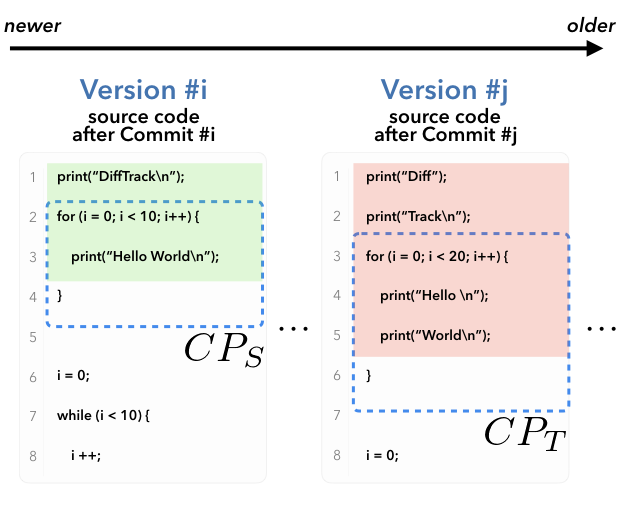
\includegraphics[width=0.9\columnwidth]{algorithm/limitation.png}
%             \caption{An example illustration of a source and true target code piece ($CP_{S}$ and $CP_{T}$). In this and following figures, red and green lines represent deleted and added lines between two versions (\#$i$ and \#$j$, $i>j$), respectively. A code piece in the newer version serves as $CP_S$ (lines in the broken frame in Version \#i). A backtrack algorithm estimates the location of $CP_{T}$ given $CP_{S}$, and runs iteratively with older commits. An estimated target code piece is denoted as $\widehat{CP_{T}}$. The ideal $\widehat{CP_{T}}$ is $CP_{T}$. This backtracking returns a series of commits associated with the code piece originally selected by the user.}

% \label{fig:CommitHistory}
%       \end{figure}

% \begin{itemize}
% \setlength{\parskip}{1mm}
% \setlength{\leftskip}{4mm}
% \setlength{\itemsep}{0cm}
% \item[DC-1.] 選択されたコード断片が過去のバージョンに含まれる場合,その位置を正確に特定する事.
% %\item[DC-2.] Run in real time regardless of the project scale and code length as well as the size of a code piece.
% \item[DC-2.] プログラミング言語(スタイルシートや設定ファイルを含む)に依存する事なく動作する事.
% \item[DC-3.] コードの行単位の粒度で動作する事.
% \end{itemize}

% \begin{itemize}
% \setlength{\parskip}{1mm}
% \setlength{\leftskip}{4mm}
% \setlength{\itemsep}{0cm}
% \item[DC-1.] Accurately identify the location of a code piece in an older version even if changes occurred within it.
% %\item[DC-2.] Run in real time regardless of the project scale and code length as well as the size of a code piece.
% \item[DC-2.] Be compatible with any type of program-related files including style sheets and configuration files.
% \item[DC-3.] Perform at a line-level granularity to support unconstrained interaction.
% \end{itemize}

% \shibato{}{source code piece を被選択コード断片,target code piece を目的コード断片と翻訳しました}

アルゴリズムを説明するために,まず被選択コード断片と目的コード断片を定義する.
被選択コード断片($CP_{S}$)は,ユーザがCodeGlassのインターフェース上で選択したコード断片である.
また目的コード断片は,過去のバージョンにおける被選択コード断片と対応したコード断片である.
アルゴリズムは$CP_{S}$の情報を受け取り,過去のバージョン内の目的コード断片の位置を推定する.
ここで,正解目的コード断片($CP_{T}$)と推定目的コード断片($\widehat{CP_{T}}$)を新たに定義する.
正解目的コード断片は過去のバージョンにおける$CP_{S}$にマッチするコード断片である.
また,推定目的コード断片はアルゴリズムが推定した過去のバージョンにおける被選択コード断片を意味する.
アルゴリズムが完全に正しく動作した場合,$\widehat{CP_{T}}$と$CP_{T}$が一致する.
% \shibato{
% また,アルゴリズムは過去のバージョン数に合わせて繰り返し実行されるため,$i$をコード断片のバージョンの順番番号と定義する.
% 即ち,$CP_{Ti}$は最新から$i$番目のバージョンにおける正解目的コード断片である.
% }{ここ使ってないので消してもいいかも}

% To explain the details of the algorithm, we first define a source and target code piece.
% A source code piece ($CP_{S}$) is a code piece in a commit.
% Using $CP_{S}$, our algorithm estimates a target code piece in an older commit.
% We denote a true and estimated target code piece as $CP_{T}$ and $\widehat{CP_{T}}$, respectively.
% Ideally, $\widehat{CP_{T}}$ is exactly the same set of lines of $CP_{T}$.
% As our algorithm is executed iteratively, an additional subscript $i$ represents a code piece in the $i$-th version from the initial commit (i.e., $CP_{Si}$ is the source code piece in Version \#$i$).
%We assume that the number of $CP_T$ is always one.

%The iteration occurs by using a target code piece as the source in the next step (i.e., $CP_{Sj} = \widehat{CP_{Ti}}$, $i>j \geq 1$).

% \subsection{Limitations with git and git-blame commands}
% \label{subsection:Limitations_with_git_commands}


%     \begin{figure}[tb]
%             \centering
%           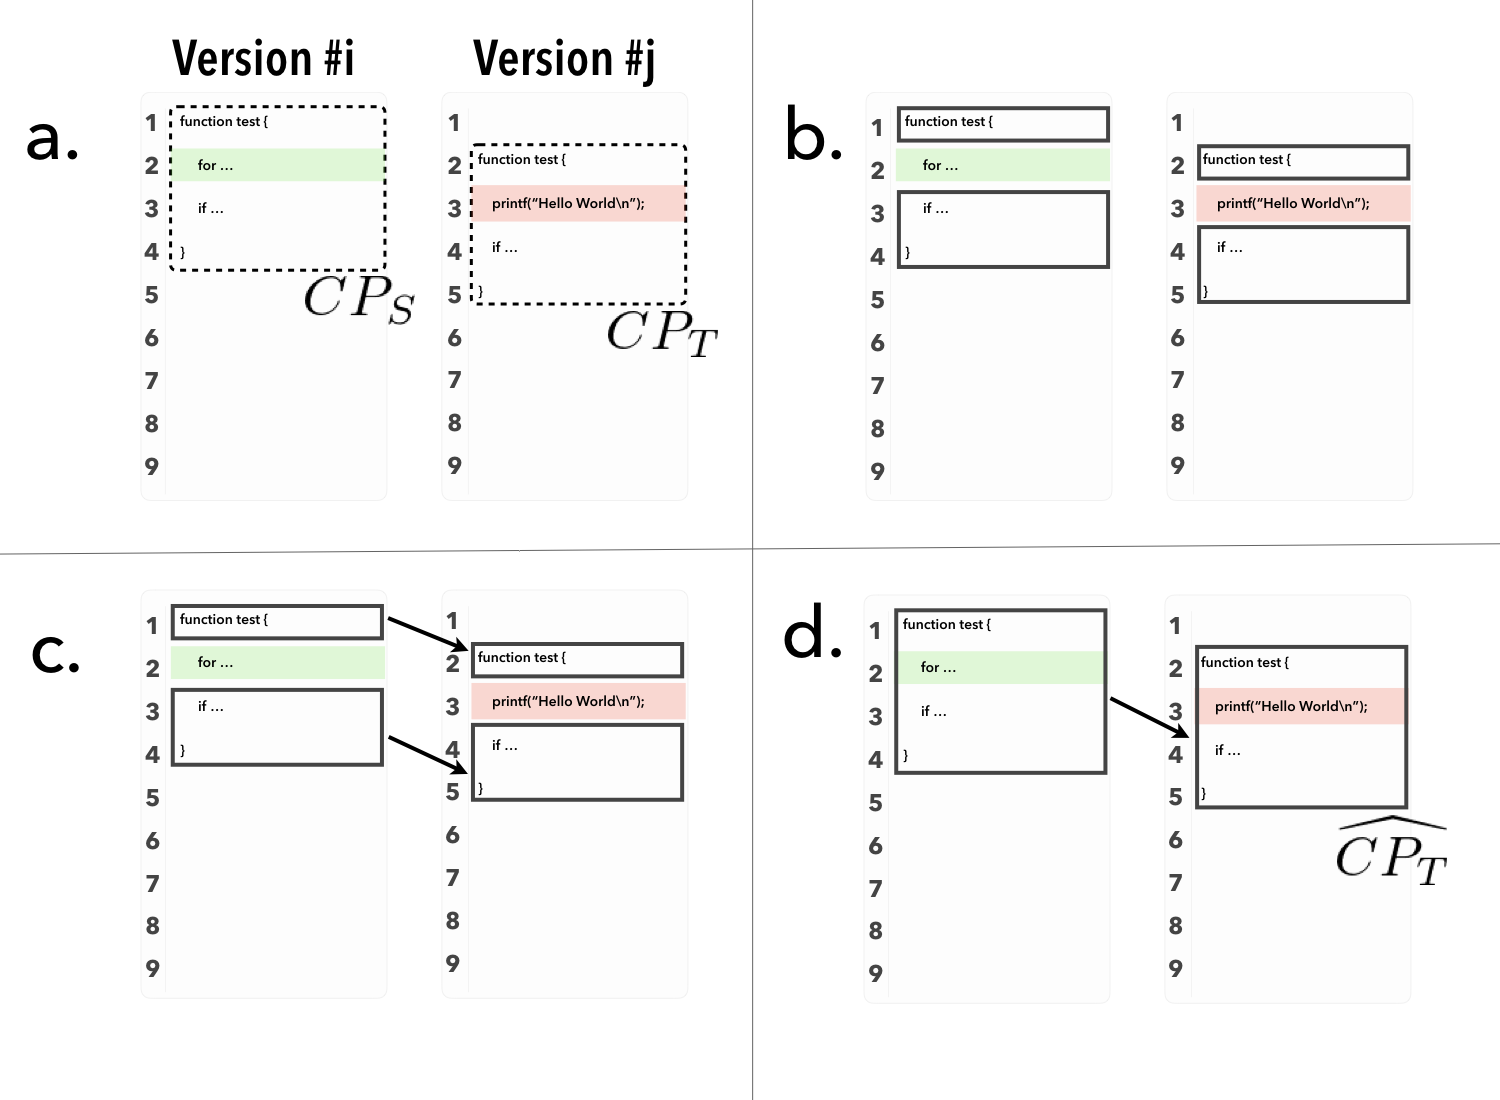
\includegraphics[width=1.0\columnwidth]{algorithm/Cases_001.png}
%           \caption{Case A: $CP_S$ includes unchanged lines that enclose the revised portion. (a) $CP_S$ and $CP_T$ are line 1--4 in the source commit and line 2--5 in the target commit, respectively. (b) The unchanged lines in $CP_S$ enclose the revised portion. (c) The unchanged lines serve as an anchor for search. (d) DiffTrack thus immediately determines line 2--5 as $\widehat{CP_T}$.}
%           \label{fig:caseA}
%     \vspace{-2mm}
%     \end{figure}


%     \begin{figure}
%       \centering
%         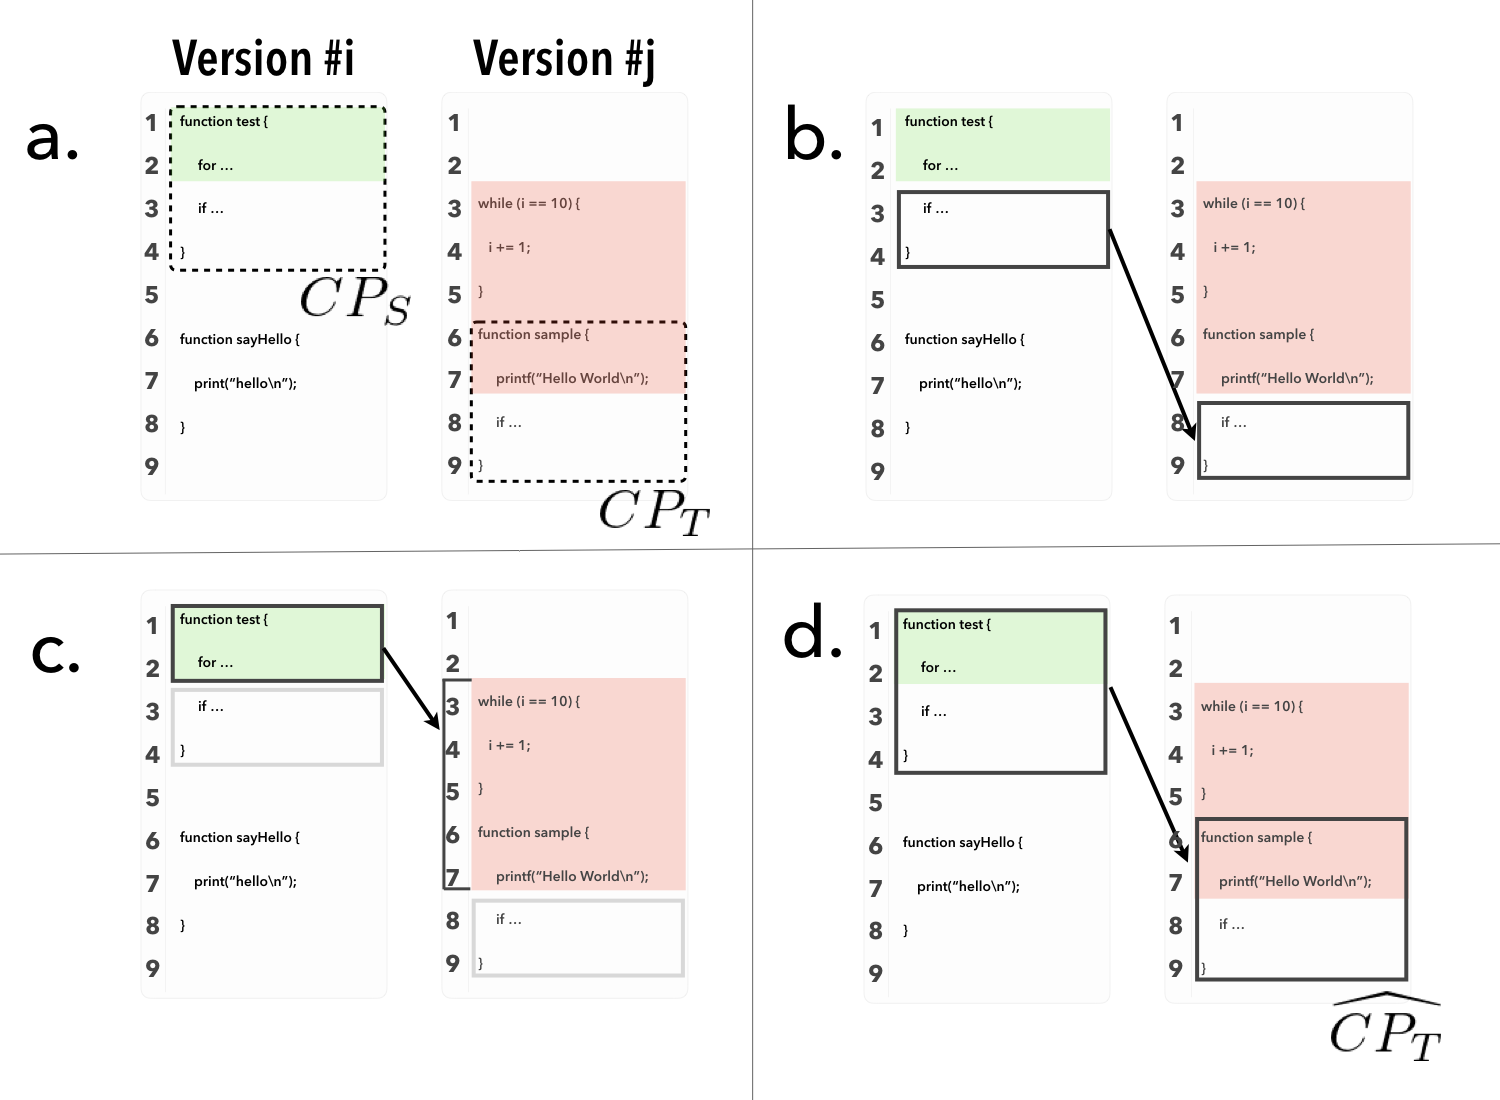
\includegraphics[width=1.0\columnwidth]{algorithm/Cases_002.png}
%         \caption{Case B: $CP_S$ includes unchanged lines that do not enclose the revised portion. (a) $CP_S$ and $CP_T$ are line 1--4 in the source commit and line 6--9 in the target commit, respectively. (b) DiffTrack first performs matching with the unchanged lines. (c) It removes unchanged lines (line 1 and 2) in the target commit from the search space. (d) It then performs fuzzy string search matching to identify lines most similar to the revised lines in the source commit. It finally determines line 6--9 $\widehat{CP_T}$.}~\label{fig:caseB}
%     \vspace{-5mm}
%     \end{figure}


% Figure~\ref{fig:CommitHistory} shows an example of code changes between two versions (\#$i$ and \#$j$, $i > j$).
% Suppose that our system needs to identify commits related to line 2--4 in Version \#$i$ to extract associated pull requests.
% Thus, this portion is $CP_{Si}$~(the broken frame in Version \#$i$ in Figure~\ref{fig:CommitHistory}).
% The git-blame command can point to the latest commit in which any part of $CP_{Si}$ was affected.
% Thus, it is straightforward to find Commit \#$j$.
% However, it provides \textit{only} the latest commit that contains changes in $CP_{Si}$.
% This means that a system needs to find $CP_{Sj}$ (or $CP_{Ti}$) given $CP_{Si}$ to trace back to older commits and iteratively perform git-blame.
% However, a diff log merely contains a set of line additions and deletions, which do not directly represent which revised lines are related to $CP_{Si}$.
% In other words, git-blame cannot immediately provide the location of $CP_{Ti}$.
% In the example of Figure~\ref{fig:CommitHistory}, a system can only know that there are three lines of additions and five lines of deletions.
% But it is not immediately clear which revised lines are related to $CP_{Si}$, and we thus need a method to estimate the location of $CP_{Ti}$ (which also serves as $CP_{Sj}$ for further backtracking).

% \subsection{Limitations with abstract syntax trees}

% Another alternative approach is to use fine-grained source code change extraction methods~\cite{GumTree, Change_Distilling}.
% These approaches can extract not only additions or deletions but also infer syntactic changes, such as updates or moves.
% They use an abstract syntax tree (AST) to compute similarity between the two versions and extract syntactic changes.
% %One example of such algorithms is Change Distiller developed by Fluri et al~\cite{Change_Distilling}.
% %Falleri et al.'s GumTree~\cite{GumTree} further improve precisions on detecting code moves.
% Although these algorithms are designed to compare multiple versions of an entire source code file, it is theoretically possible to implement them to perform matching of code pieces.


% Nevertheless, we decided not to consider AST-based methods because they do not satisfy DC-2 and 3 in general.
% As methods using abstract syntax trees require a parser, additional configuration is necessary for adaptation to different programming languages.
% For example, GumTree~\cite{GumTree} is only compatible with C, Java, JavaScript, and Ruby as of April 2017.
% Internal parsing can lead to large computational overhead for long code pieces.
% In addition, a selected code piece should be syntactically correct, which also limits user experience.
% We thus developed an algorithm called DiffTrack.

% \koji{}{If we have anything besides LHDiff to be discussed, add it here and explain why we don't use it.}

先行研究では,コード断片を過去のバージョンの中で追跡する手法が提案されており,それらをCodeGlassのサーバのアルゴリズムとして活用できる可能性がある.
% 例えばSpaccoとWilliams~\cite{SDiff}が実装したSDiffというアルゴリズムは,抽象構文木を用いてコードを解析する事で,コード断片を過去のバージョンの中で追跡する事ができる.
% しかし,SDiffが動作するためには構文解析を行う必要があるため,DC-2を満たす事が出来ない.
Asaduzzamanら~\cite{LHDiff}が開発したLHDiffは,プログラミング言語非依存で動作するコード断片追跡アルゴリズムである.
LHDiffはword-level fuzzy matching~\cite{sankoff1983time}を用いて$CP_{S}$と$\widehat{CP_T}$との文字列的類似度を計算し,最も類似度が高かったものを$CP_{T}$として決定する.
%LHDiffは要件DC-2とDC-3を満たしており,かつ評価実験ではその他のコード断片追跡アルゴリズムよりも正確であった事から,要件DC-1も満たしている.

% 過去のバージョン内でコード断片を追跡するアルゴリズムに関する先行研究が複数存在する.
% SpaccoとWilliams~\cite{SDiff}が実装したSDiffというアルゴリズムは,抽象構文木を用いてコード断片を追跡する事ができる.
% SDiffが動作するためには構文解析を行う必要があるため,プログラミング言語に依存する.
% 一方でAsaduzzamanら~\cite{LHDiff}が開発したLHDiffは,プログラミング言語非依存で動作するコード断片追跡アルゴリズムである.
% LHDiffは\shibato{fuzzy string matching}{日本語にする必要ある?}を使用しコード断片と$\widehat{CP_T}$の候補との文字列的類似度をそれぞれ計算する事で,$\widehat{CP_T}$を推定する.
% そして最も類似度が高かったコード断片を$\widehat{CP_T}$として決定する.
% LHDiffは要件DC-2とDC-3満たしており,かつAsaduzzamanらによる評価実験ではその他のコード断片追跡アルゴリズムよりも正確であった事から,要件DC-1も満たしている.

% There exist different algorithms for backtracking code changes across revisions.
% SDiff developed by Spacco and Williams~\cite{SDiff} uses abstract syntac trees for backtracking.
% This algorithm requires syntactic analysis, and thus it is language-dependent.
% In contrast to SDiff, Asaduzzaman et al. demonstrated a language-agnostic algorithm, called LHDiff~\cite{LHDiff}.
% It uses fuzzy string matching and calculates similarity between the given code piece and candidates of $\widehat{CP_T}$.
% LHDiff then determines $\widehat{CP_T}$ as a code piece with the highest similarity score.
% This algorithm satisfies DC-2 and DC-3.
% In addition, their evaluation showed that LHDiff achieves a high accuracy performance compared to other code tracking techniques and thus meets DC-1.

しかし我々がLHDiffの事前調査を行った結果,コード変更が構造的変更(関数の統合や分裂,リファクタリングなど)を含む場合,LHDiffはコード断片の追跡に失敗する事が分かった.
この原因は,LHDiffでは$CP_T$が一つしか存在しないと仮定されているからである.
実際のコード変更履歴では,被選択コード断片が過去のバージョンにおいて他のコード断片と統合されていたり,分割されて実装されていたりする可能性がある.
特に大規模なソフトウェア開発プロジェクトでは,ソースコードの構造的変更が繰り返し行われる事が多いため,LHDiffをそのままCodeGlassのサーバに実装すると,CodeGlassの実用性が制限されてしまう.
そこで我々は,LHDiffに新たにgraceful matchingを導入することでこの問題を解決することを試みた.

% However, our pilot study on the na\"{i}ve LHDiff method found that it fails to backtrack when revisions involve structural changes (e.g., merge and refactoring) because it assumes that the number of $CP_T$ is always one.
% This may cause degradation of the utility of CodeGlass.
% To address this issue, we integrated a graceful code matching mechanism into LHDiff.


LHDiffは$CP_T$が常に一つであるという仮説の下,最も文字列的類似度が高いコード断片を$\widehat{CP_T}$として決定する.
我々は新たに,正解目的コード断片が一つに定まる可能性が高い事を示す閾値であるDMT(Definitive Matching Threshold)を導入した.
$CP_{S}$と$\widehat{CP_T}$の候補の文字列的類似度がDMTよりも高かった場合,LHDiffと同様に$\widehat{CP_T}$を決定する.
しかし,過去にソースコードの構造的な変更や大規模な修正が行われていると,文字列的類似度が低くなり,$CP_{T}$を正確に一意に推測する事が難しくなる.
そこで,別の閾値であるCMT(Candidate Matching Threshold)を導入する.
DMTを上回る$\widehat{CP_T}$が存在しなかった場合,CMTを上回るコード断片を全て,$CP_{T}$である可能性があるとしてインターフェースに返す.
CodeGlassのインターフェースは,それらのコード断片を含むコミットを図~\ref{fig:WebInterface}a~(3)のように表示する.
ユーザはそのコミットをクリックして過去のバージョンにおけるソースコードを確認し,$CP_S$として選択し直す事で,引き続きコード断片の調査を継続する事ができる.
% ユーザはそのコミットをクリックして過去のバージョンにおけるソースコードを確認し,\sakaguchi{$CP_{T}$を特定してから}{ユーザが正解目的コード断片を特定するというのに違和感を覚えます…CPtはあくまで学習におけるシンボルな気がします}それを$CP_S$として選択し直す事で,引き続きコード断片の調査を継続する事ができる.

% The na\"{i}ve LHDiff method determines $\widehat{CP_T}$ as a code piece with the highest similarity under an assumption that the number of $CP_T$ is always one.
% We introduce a threshold (Definitive Matching Threshold, DMT) to determine if there exists a single possible target code piece with strong belief.
% But the fuzzy string matching method may still fail to find a single $\widehat{CP_T}$ when changes are substantial.
% To allow graceful matching, we introduce another threshold (Candidate Matching Threshold, CMT).
% The graceful matching creates a list of likely target code pieces instead of simply stopping search.


DMTとCMTの二つの閾値を設定するために,Chart.jsのリポジトリに含まれる49個のコミットにおける,変更前と変更後のコード断片の一対をデータセットとして構築した.
このデータセットではLHDiffだけでは$CP_{T}$を特定する事が難しい構造的変更からなるコミットのみを意図的に選定した.
そして,それぞれのコード断片に対して$CP_S$を選択し,それに対応する$CP_T$のラベル付けを行った.
% そして,それぞれのコード断片に対して\sakaguchi{$CP_S$}{そういえば学習におけるCPsはどう決めるんでしょう?}と$CP_T$のラベル付けを行った.
さらに,$CP_T$と最も文字列的類似度の高い,$CP_T$ではないコード断片を$IM$(incorrect match)としてラベル付けした.
% \sakaguchi{}{目的コード断片の定義がちゃんとわかっていないのですが単純に似たコードということでしょうか…?ちなみに同じ内容の断片が複数ファイルに合った場合どうなるでしょう…?}


% To determine appropriate values for these threshold, we created a dataset containing 49 commits (i.e., 49 pairs of two versions) in Chart.js.
% This dataset deliberately contained only refactoring revisions.
% Estimating a match in these revisions is presumably difficult with the na\"{i}ve LHdiff algorithm.
% In each pair, we manually labeled $CP_S$ and $CP_T$.
% We also chose a code piece which was a disjoint set of $CP_T$ and exhibited the highest similarity as the most similar incorrect match ($IM$).

図~\ref{fig:histogram_sim}に$CP_T$(青)と$IM$(橙)の文字列的類似度の分布を示す.
この分布から$IM$の類似度は0.65未満である事が分かる.
また,$CP_T$の類似度は0.4より大きい事も分かる.
したがって我々は,DMTを0.65に,CMTを0.4に設定した.

% Figure~\ref{fig:histogram_sim} shows the distributions of similarity scores of $CP_T$ (in blue) and $IM$ (in pale orange).
% This histogram clearly illustrates that similarity scores of $IM$ are below 0.65.
% It also shows that the scores of $CP_T$ are above 0.45.
% We, therefore, determined DMT and CMT to be 0.65 and 0.4, respectively.


% 我々のコード断片追跡アルゴリズムは,ユーザが選択したコード断片内でのコード変更を含むコミットの一覧を特定する.
% アルゴリズムはまず最初に,git-blameを用いてコード断片の最新のコミットを特定する.
% 次にLHDiffにより最も文字列的類似度の高いコード断片を$\widehat{CP_T}$として決定する.
% この処理を繰り返し行い,DMTを上回るコード断片が見つからなかった時に動作を終了する.

% Our tracking algorithm can identify a set of commits that contain changes on a user-selected code piece.
% It first finds the latest commit containing changes on the code piece by the git-blame command.
% LHDiff then locates a portion of code in this version which is the most similar to the given code piece (i.e., $\widehat{CP_T}$).
% It then performs this operation iteratively by using the estimated portion of code as the next source code piece to trace back to even older versions.
% Our algorithm stops backtracking when it finds no code piece with a higher value than DMT.

% \shibato{graceful matching}{}は,追加でCMTを上回る正解目的コード断片の可能性があるコード断片を探索する.
% コード断片がコミットにおいて別ファイルへ移動した可能性も考慮して,\shibato{graceful matching}{}は変更のあった全てのファイルを探索する.
% そして見つかった正解目的コード断片の可能性があるコード断片を文字列的類似度順に並び替える.
% 次にそれらのコード断片が互いに排他的である事を確認してから,インターフェースに返す.
% インターフェース上では正解目的コード断片の可能性があるコード断片はFigure~\ref{fig:WebInterface}a(2)のように示される.

% With graceful matching, the algorithm additionally searches all possible code pieces with the similarity scores above CMT after backtracking.
% In order to capture cases in which a code piece was moved from a file to another, the graceful matching process checks all revised files in the repository. 
% The algorithm first sorts possible target code pieces by their similarity scores in the descending order, and initializes a list for candidate target code pieces.
% For each possible code piece, the algorithm checks if it is mutually exclusive with all lines in the current candidate list.
% If true, the algorithm adds that code piece to the candidate list.
% All code pieces in this candidate list are finally shown to the user in the interface ((2) in Figure~\ref{fig:WebInterface}a).


% \subsubsection{Case A: $CP_S$ includes unchanged lines that enclose the revised portion.}


% $CP_S$ contains revised lines between the unchanged portions (i.e., line 2 in Version \#i in Figure~\ref{fig:caseA}).
% In this case, the algorithm first uses the unchanged lines (line 1, 3, and 4) as an anchor to find $\widehat{CP_T}$.
% In addition, only changed lines should be included between the unchanged portions.
% The algorithm, therefore, immediately identifies $\widehat{CP_T}$ as the unchanged portions and changed lines in-between (i.e., line 2--5 in Version \#$j$).

% \subsubsection{Case B: $CP_S$ includes unchanged lines that do not enclose the revised portion.}

%     \begin{figure}[tbp]
%             \centering
%           \includegraphics[clip, width=8cm]{algorithm/CaseB.png}
%           \caption{An example of case B (where $CP_S$ includes unchanged lines that do not enclose the revised portion).
%           $CP_S$ and $CP_T$ are from line 1 to 4 in the source commit and from line 6 to 9 in the target commit, respectively.~(a)
%           The algorithm first perform matching with the unchanged lines.
%           In this example, codes from line 3 to 4 in the source commit matches with counterparts from line 8 to 9 in the target commit.~(b)
%           The algorithm removed unchanged lines from the target commit (i.e., line from 1 to 2 in the target commit) to prune the search space.~(c)
%           It then performs fuzzy string search matching to identify codes most similar to the revised lines~(i.e., line 1 and 2 in the source commit).
%           The algorithm finally determines from line 6 to 9 in the target commit as $CP_T$.~(d)
%           }
%           \label{fig:caseB}
%     \end{figure}


% $CP_S$ contains unchanged lines, but the revised portion is not enclosed.
% Figure \ref{fig:caseB} presents such an example where the first half has been revised while the other stays unchanged.

% Similar to the previous case, the algorithm first performs matching with the unchanged lines.
% This matching result narrows down the possible lines for $\widehat{CP_T}$ (above line 7 in this example).
% The algorithm further reduces the search space by removing remaining unchanged lines because it can assume that the rest of $\widehat{CP_T}$ should be revised lines.
% In this example, line 1 and 2 are unchanged, and thus they are removed from the search.
% The algorithm then performs fuzzy string matching between the revisions (explained in detail later), and identifies the set of lines with the highest similarity score (line 6 and 7 in this example).
% DiffTrack determines line 6--9 as $\widehat{CP_T}$.


% \subsubsection{Case C: $CP_S$ does not include unchanged lines.}

%     \begin{figure}[tbp]
%             \centering
%           \includegraphics[clip, width=8cm]{algorithm/CaseC.png}
%           \caption{An example of case C (where $CP_S$ does not include unchanged lines).
%           $CP_S$ and $CP_T$ are from line 1 to 3 in the source commit and from line 5 to 7 in the target commit, respectively.~(a)
%           The algorithm first removes all unchanged lines from the target commit.~(b)
%            It then performs fuzzy string matching on all possible string chunks, and finds the most similar match.~(c)
%            The algorithm finally determines codes from line 5 to 7 in the target commit as $CP_T$.~(d)}
%           \label{fig:caseC}
%     \end{figure}

% \begin{figure}
%     \centering
%       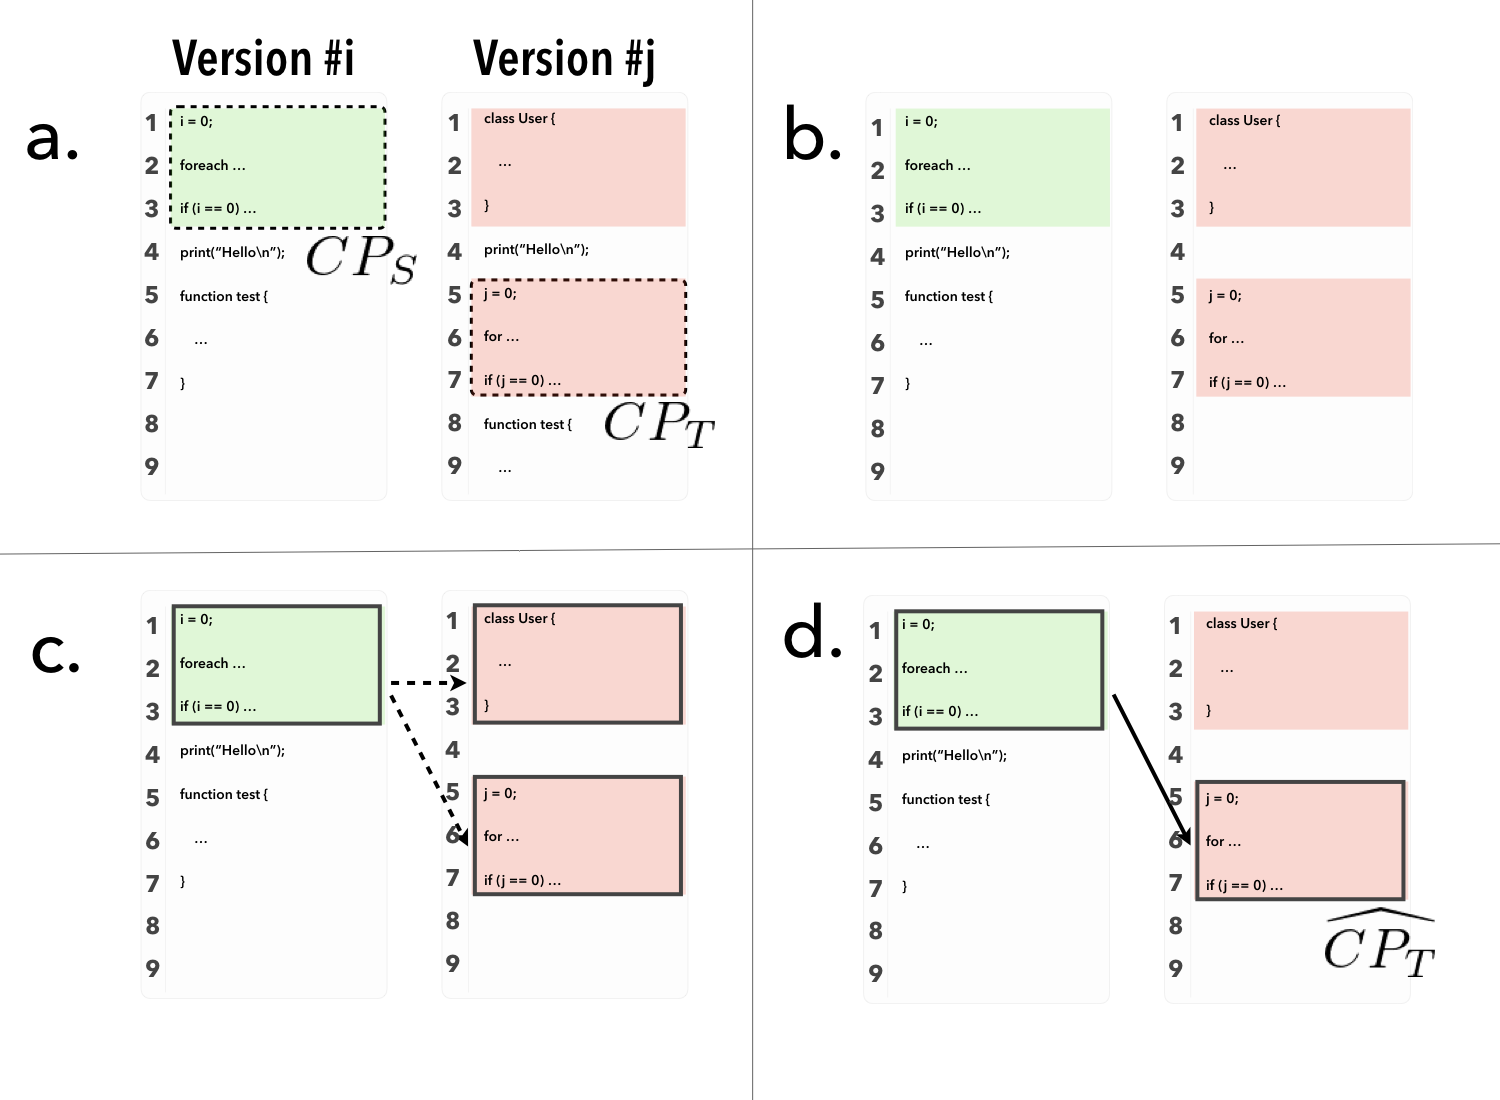
\includegraphics[width=1.0\columnwidth]{algorithm/Cases_003.png}
%       \caption{Case C: $CP_S$ does not include unchanged lines (a) $CP_S$ and $CP_T$ are line 1--3 in the source commit and from line 5--7 in the target commit, respectively. (b) DiffTrack first removes all unchanged lines from the search. (c) It then performs fuzzy string matching on all possible string chunks, and finds the most similar match. (d) DiffTrack finally determines line 5--7 in the target commit as $\widehat{CP_T}$.}~\label{fig:caseC}
%     \vspace{-5mm}
%     \end{figure}



% The two example above demonstrates that unchanged lines in $CP_S$ serve as a useful anchor for determining $\widehat{CP_T}$.
% However, $CP_S$ may not contain any unchanged line as illustrated in Figure \ref{fig:caseC}.
% In this case, DiffTrack first removes all unchanged lines from the search.
% This would result in string chunks (i.e., sets of consecutive code lines) as shown in Figure \ref{fig:caseC}.
% The algorithm then performs fuzzy string matching on all chunks and sub-chunks, and finds the most similar match.

% \subsection{Fuzzy String Matching}
% The DiffTrack algorithm performs fuzzy string matching to identify a code piece most similar to $CP_S$ in the target commit.
% It uses a variant of the Levenshtein distance as a cost function.
% The Levenshtein distance is defined as the minimum number of character operations that are necessary to convert a string to another.
% Character operations include additions, deletions and substitutions.
% In our fuzzy string matching, we calculate the distance on a word basis with different weights on change operations (1, 1, and 2 for additions, deletions and substitutions, respectively).
% For example, the cost of a conversion from ``int x = 1 + 2;'' to ``float x = 1.0;'' is 6 because there are 2 deletions and 2 substitutions.
% Our fuzzy matching also considers the length of $CP_S$ and a possible target code piece ($cp$).
% The DiffTrack algorithm thus uses the following similarity score to find possible a target code piece:

% % \koji{}{Maybe explain why we use word-based similarity rather than char-based?}

% \vspace{-5mm}
% \begin{equation*}
% Sim(cp) = \frac{wp(CP_S) + wp(cp) - LDw(CP_S,\, cp)}{wp(CP_S) + wp(cp)},
% \end{equation*}
% \vspace{-3mm}

% where $wp(x)$ is the word count in text $x$, and $LDw$ is a word-level Levenshtein distance.
% $Sim(cp)$ takes a value between 0 and 1, representing that higher is more similar.
% We use a brute-force approach to find a code piece with the highest similarity score.





\begin{figure}[t]
\centering
  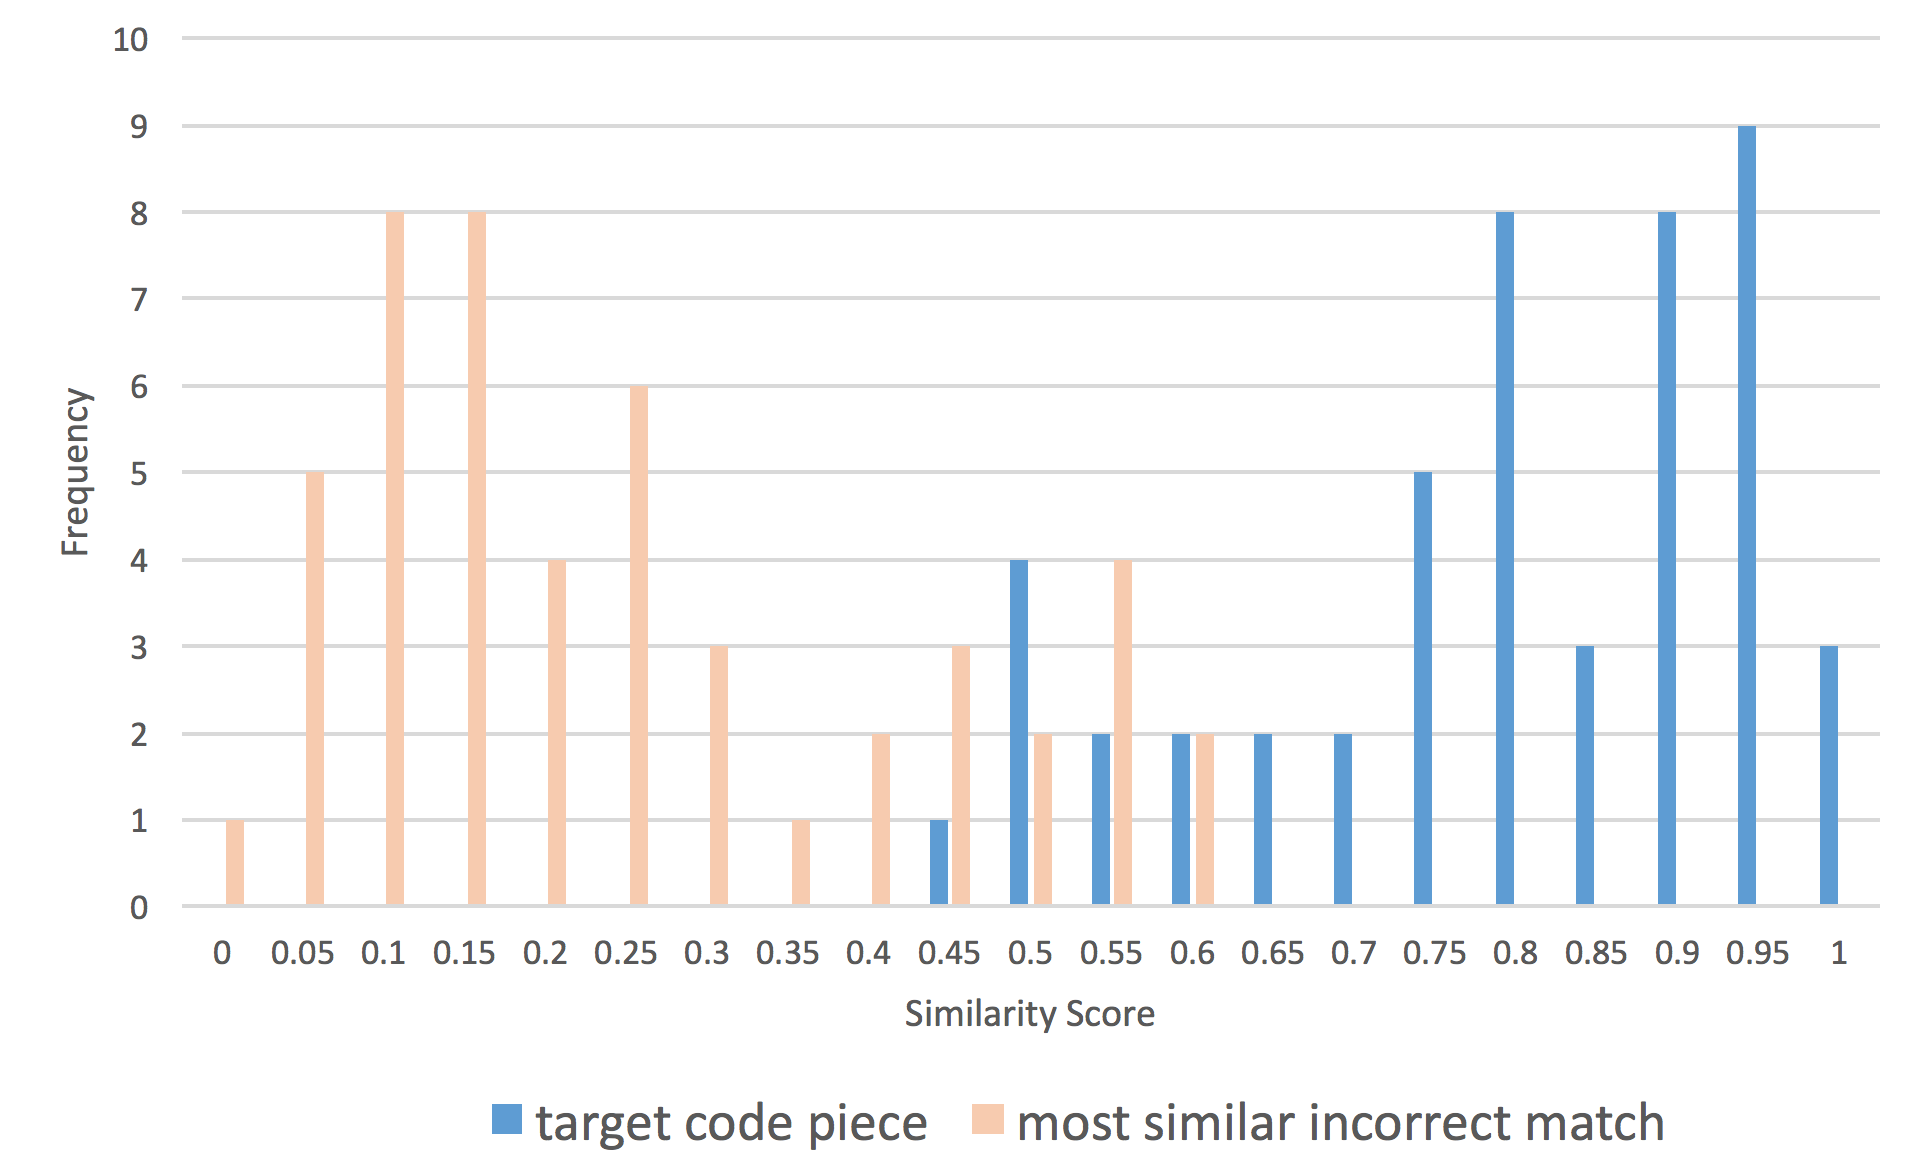
\includegraphics[width=1.0\columnwidth]{algorithm/histogram_sim.png}
  \caption{$CP_T$(青)と$IM$(橙)の文字列的類似度の分布.}~\label{fig:histogram_sim}
\end{figure}











\begin{figure*}[t]
  \centering
  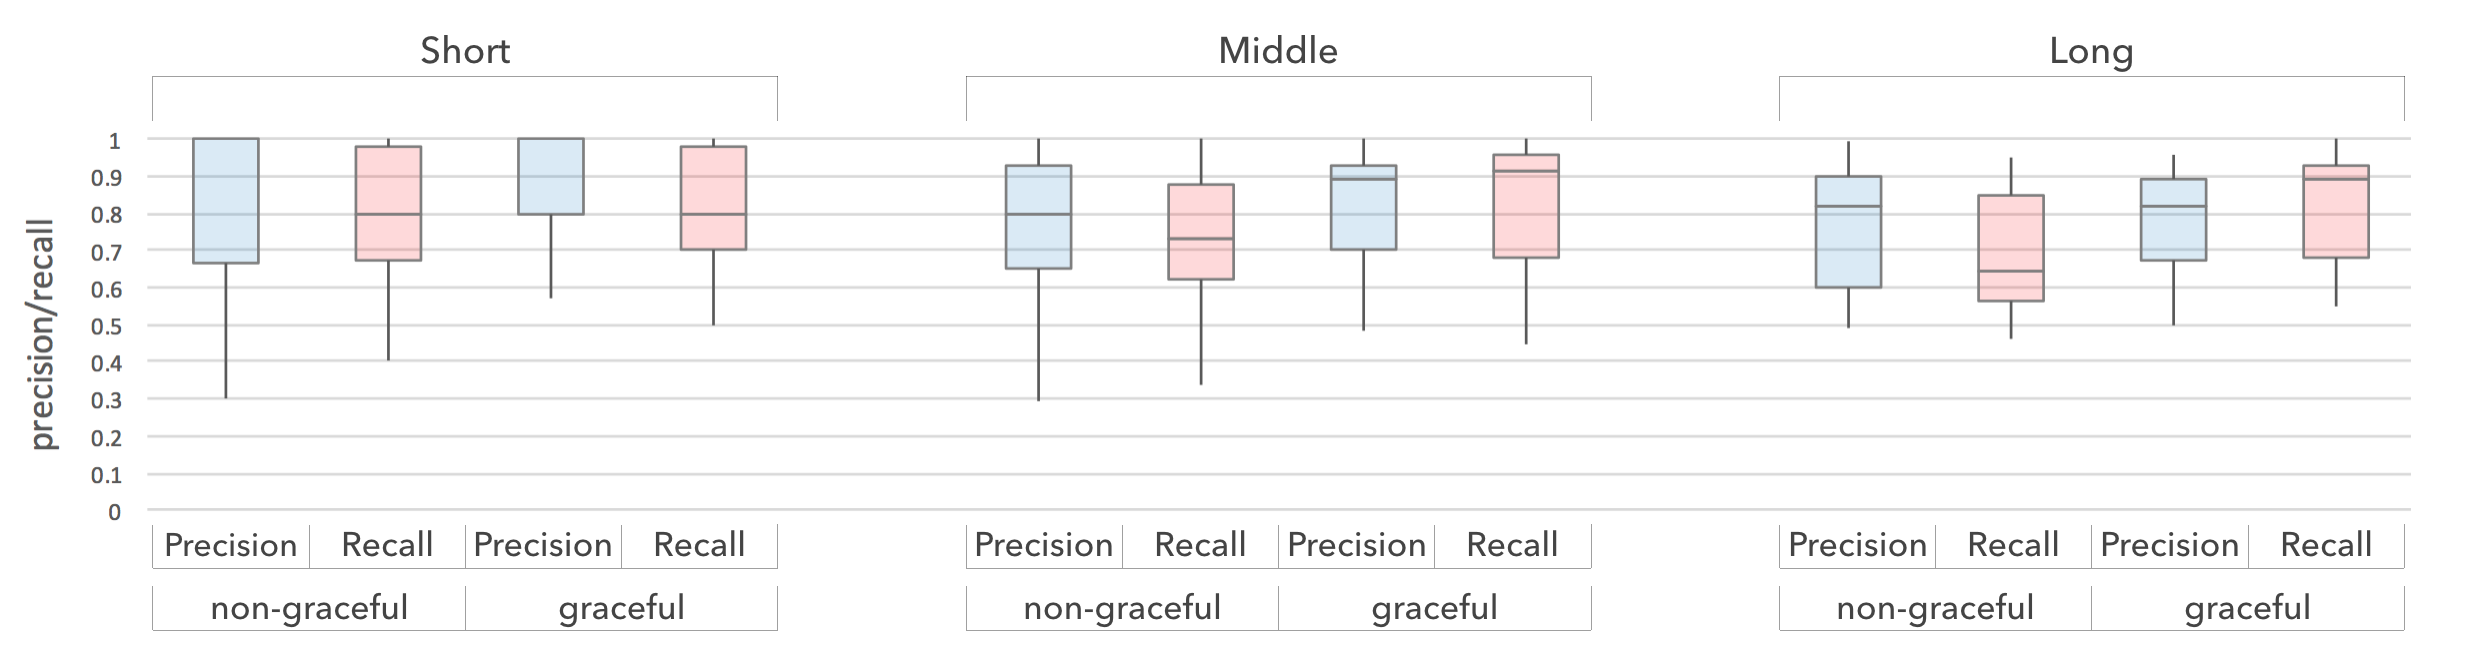
\includegraphics[width=2.0\columnwidth]{evaluate/difftrack_eval_commit.png}
  \caption{graceful matchingのコード断片の特定精度の評価の結果.\textit{Short}グループの適合率は,graceful matchingを用いた場合,用いなかった場合の両方において中央値が1.0であった.}~\label{fig:Commit_Matching_Accuracy_Evaluation}
%   \caption{Box plots of code matching accuracy performance results with our backtrack algorithm. Note that the medians for the precision under the \textit{Short} condition were 1.0 both with and without graceful matching.}~\label{fig:Commit_Matching_Accuracy_Evaluation}
  \vspace{-5mm}
\end{figure*}

\subsection{改良アルゴリズムの定量的評価}

graceful matchingが目的コード断片の特定の精度をどの程度改善するのかを明らかにするために,我々はGitHubの実際のコード変更データを用いた定量的評価を行った.
はじめにChart.jsのリポジトリから100個のコード断片を選択し,それらを\textit{Short}(9行以下,34個のコード変更),\textit{Middle}(10行以上30行以下,33個のコード変更),そして\textit{Long}(31行以上,33個のコード変更)の3つのグループに分類した.
次にそれら100個の原コード断片の開発履歴を辿り,5つ以上の過去のバージョンにおけるコード断片を抽出し,原コード断片と組み合わせる事で評価用のデータセットを構築した.
そして,過去のコード断片を特定する精度をgraceful matchingの有無で比較評価した.


% To understand how much the graceful matching improves target code piece identification, we conducted a quantitative evaluation using real code revision data obtained from open source repositories on GitHub.
% % We have two objectives for our evaluations: 1) to quantify how accurately the algorithm can estimate a code piece; and 2) to quantify how accurately the algorithm can extract a set of commits given a code piece.
% We chose 100 code pieces with various length of changes from the Chart.js repository, and divided into three groups: 34 \textit{Short} ($\sim 9$ lines), 33 \textit{Middle} ($10 \sim 30$ lines), and 33 \textit{Long} ($30 \sim$ lines).
% We then manually traced back the development history, and created the ground truth data consisting of more than five commits associated with each original source code piece.
% We evaluated the accuracy of selected commits with and without the graceful matching.

評価指標として適合率($P_{cp}$)と再現率($R_{cp}$)を用いた.
$l_c$を$\widehat{CP_{T}}$として正しく推定されたのコード行数,$l_i$を$\widehat{CP_{T}}$として間違って推定されたコードの行数,$l_n$を$CP_{T}$に含まれるが$\widehat{CP_{T}}$には含まれてないコードの行数とした時,適合率と再現率は$P_{cp} = \frac{l_c}{l_c + l_i},\;\; R_{cp} = \frac{l_c}{l_c + l_n}$と定義した.  

% We used precision and recall ($P_{cp}$, $R_{cp}$) as performance metrics.
% More specifically, $P_{cp} = \frac{l_c}{l_c + l_i},\;\; R_{cp} = \frac{l_c}{l_c + l_n},$ where $l_c$, $l_i$, and $l_n$ represent the numbers of lines correctly included in $\widehat{CP_{T}}$; lines incorrectly included in $\widehat{CP_{T}}$; and lines that are in $CP_{T}$ but not in $\widehat{CP_{T}}$, respectively.

図~\ref{fig:Commit_Matching_Accuracy_Evaluation}が示すように,全ての条件においてgraceful matchingを用いることで適合率と再現率が改善された.
また,適合率及び再現率の結果とgraceful matchingの有無に対して重回帰分析を行った結果,適合率が再現率が有意に改善されたことが分かった.
適合率における回帰係数は0.058($SE=0.025$, $p<.05$),再現率における回帰係数は0.051($SE=0.021$, $p<.05$)であった.
さらに,\textit{Short}グループの方が\textit{Long}のグループと比較して,有意に高い適合率及び再現率であった($p<.05$).

% Figure~\ref{fig:Commit_Matching_Accuracy_Evaluation} summarizes the results, showing that the performance was high across all the conditions.
% We ran multi-level linear regression analysis with two factors: the length group and the presence of graceful matching.
% The result showed that graceful matching significantly improved precision and recall.
% The estimated coefficients were 0.058 ($SE=0.025$, $p<.05$) and 0.051 ($SE=0.021$, $p<.05$) for precision and recall, respectively.
% \textit{Short} also showed significantly higher precision and recall than \textit{Long} ($p<.05$).

graceful matchingの評価を行った結果,コード断片の特定における適合率および再現率を約5\%改善できたことが分かった.
また図~\ref{fig:Commit_Matching_Accuracy_Evaluation}に示すように,graceful matchingが頑健性に貢献することが示された.
例えば,ある1つのデータでは,LHDiffのみの場合適合率と再現率がそれぞれ0.30と0.40であったが,graceful matchingを適用することで両方ともに0.80まで改善したことが確認された.
graceful matchingはコード断片の特定の精度を改善することができるため,我々はgraceful matchingをCodeGlassに導入することとした.

% The results suggest that our graceful approach can improve precision and recall of identifying commits by roughly 5\% in our dataset.
% Although the effect estimated by our multi-level linear regression was not large, it offers robustness to cases in which the default backtrack algorithm exhibits low precision and recall as shown in Figure~\ref{fig:Commit_Matching_Accuracy_Evaluation}.
% In one test case, the na\"{i}ve LHDiff algorithm was only able to achieve the precision and recall of 0.30 and 0.40, respectively, but the graceful approach improved both of them to 0.80.
% We thus concluded that the graceful approach can improve commit matching and should be included in the CodeGlass system.







\section{定量的ユーザ評価実験}
\label{section:user-study}
% \section{Comparative User Evaluation}


% We next conducted a user evaluation to investigate how CodeGlass can support comprehension of code pieces. 

%\subsection{実験内容}
% \subsection{Experiment Design}

% Existing tools already support Contributor and Usage information seeking (e.g., git-blame to identify who made a particular change).
% Therefore, we decided to mainly examine the user performance of finding information for \textbf{Execution}, \textbf{Rationale}, and \textbf{History} in our evaluation.
% These information categories were also found important by the professional developers in our formative study.

% \begin{table*}[t]
%     \centering
%      \caption{Accuracy performance and confidence scores in the user evaluation. Values in parentheses represent the standard deviations.}
%     \label{table:experiment_result}
%     \begin{tabular}{c||ccc|ccc} \Hline
%     \multirow{2}{*}{Category} & \multicolumn{3}{c|}{\textbf{without CodeGlass}} & \multicolumn{3}{c}{\textbf{with CodeGlass}} \\
%      & Precision & Recall & Confidence & Precision & Recall & Confidence \\ \hline \hline
%      Execution & 0.77 (0.12) & 0.46 (0.08) & 74.5 (9.67) & 0.80 (0.18) & 0.49 (0.13) & 79.6 (7.14) \\
%      Rationale & 0.55 (0.38) & 0.14 (0.09) & 63.9 (28.1) & 0.79 (0.21) & 0.29 (0.06) & 78.3 (11.6) \\
%      History & 0.13 (0.35) & 0.01 (0.02) & 6.25 (17.7) & 0.88 (0.13) & 0.16 (0.01) & 66.6 (6.25) \\ \Hline
%     \end{tabular}
% \end{table*}

\begin{table*}[t]
    \centering
     \caption{適合率,再現率,自信度の平均.但し,括弧内は標準偏差である.3つの条件は,GitHub上のインタフェース(non-CG),開発背景と理由の並べ替え機能がないCodeGlass(CG-),並べ替え機能を持つCodeGlass(CG)である.}
    \label{table:experiment_result}
    \begin{tabular}{c||ccc|ccc|ccc}  \Hline
      \multirow{2}{*}{}  & \multicolumn{3}{c|}{ \textbf{non-CG} } & \multicolumn{3}{c|}{ \textbf{CG-} } & \multicolumn{3}{c}{ \textbf{CG} } \\
      & 適合率 & 再現率 & 自信度 & 適合率 & 再現率 & 自信度 & 適合率 & 再現率 & 自信度 \\ \hline \hline
      Execution & 0.93  (0.09) & 0.45  (0.18) & 61.1 (10.7) & 0.87 (0.13) & 0.44 (0.23) & 66.4 (11.7) & 0.90 (0.11) & 0.53 (0.24) & 77.5 (10.9) \\
      Rationale & 0.86 (0.30) & 0.17 (0.09) & 63.7 (10.4) & 0.95 (0.11) & 0.31 (0.12) & 63.4 (10.5) & 0.89 (0.15) & 0.34 (0.17) & 66.8 (8.07) \\
      History & 0.08 (0.29) & 0.01 (0.04) & 30.7 (16.9) & 0.50 (0.52) & 0.14 (0.12) & 58.9 (19.3) & 0.33 (0.49) & 0.12 (0.15) & 63.7 (24.7) \\ \Hline
      \end{tabular}
\end{table*}

% \begin{table}[t]
%     \centering
%     \caption{Paired t tests on user evaluation performance results.}
%     \label{table:stats_result}
%     \begin{tabular}{rl||ccc}
%     \multicolumn{2}{l||}{Metric} & $t(7)$ & $p$ & Cohen's $d$ and 95\%CI \\ \hline \hline
%     \multicolumn{2}{l||}{\textbf{Execution}} & & & \\
%     & Precision & 0.76 & \textit{n.s.}%0.47
%     & 0.27 [-0.44, 0.97] \\
%     & Recall & 0.74 & \textit{n.s.}%0.48 
%     & 0.26 [-0.45, 0.96] \\
%     & Confidence & 1.77 & \textit{n.s.}%0.12 
%     & 0.63 [-0.16, 1.37] \\ \hline
%     \multicolumn{2}{l||}{\textbf{Rationale}} & & & \\
%     & Precision & 1.79 & \textit{n.s.}%0.12 
%     & 0.63 [-0.15, 1.38] \\
%     & Recall & 3.55 & < 0.01 & 1.25 [0.28, 2.18] \\
%     & Confidence & 1.57 & \textit{n.s.}%0.16 
%     & 0.55 [-0.21, 1.29]\\ \hline
%     \multicolumn{2}{l||}{\textbf{History}} & & & \\
%     & Precision & 4.58 & < 0.01 & 1.62 [0.52, 2.68] \\
%     & Recall & 5.97 & < 0.001 & 2.11 [0.81, 3.38] \\
%     & Confidence & 5.41 & < 0.001 & 1.91 [0.69, 3.09] \\ 
%     \end{tabular}
    
% \end{table}

% \begin{table}[t]
%     \centering
%     \caption{反復測定の一元配置分散分析の結果.}
%     \label{table:stats_result}
    
%     \begin{tabular}{ccccc} \Hline
%         \multicolumn{2}{c}{ 要因 } & df & $F$ & $p$ \\ \hline \hline
        
%         \multicolumn{5}{l}{ \textbf{Execution} - 適合率 } \\
%         	& CodeGlass & 22 & 1.71 & 0.2 \\  \hline
%         \multicolumn{5}{l}{ \textbf{Execution} - 再現率 } \\
%         	& CodeGlass & 22 & 0.47 & 0.63 \\  \hline
%         \multicolumn{5}{l}{ \textbf{Execution} - 自信度 } \\
%         	& CodeGlass & 22 & 4 & $<.005$ \\  \hline
%         \multicolumn{5}{l}{ \textbf{Rationale} - 適合率 } \\
%         	& CodeGlass & 22 & 0.73 & 0.49 \\  \hline
%         \multicolumn{5}{l}{ \textbf{Rationale} - 再現率 } \\
%         	& CodeGlass & 22 & 6.51 & $<.005$ \\  \hline
%         \multicolumn{5}{l}{ \textbf{Rationale} - 自信度 } \\
%         	& CodeGlass & 22 & 1.17 & 0.33 \\  \hline
%         \multicolumn{5}{l}{ \textbf{History} - 適合率 } \\
%         	& CodeGlass & 22 & 2.71 & 0.09 \\  \hline
%         \multicolumn{5}{l}{ \textbf{History} - 再現率 } \\
%         	& CodeGlass & 22 & 4.18 & $<.005$ \\  \hline
%         \multicolumn{5}{l}{ \textbf{History}- 自信度 } \\
%         	& CodeGlass & 22 & 9.68 & $<.005$ \\  \Hline
        
%     \end{tabular}
% \end{table}


\begin{table}[t]

    \centering
    \caption{反復測定の一元配置分散分析の結果.}
    \label{table:stats_result}
    
\hspace*{-0.23cm}    
\begin{tabular}
    {@{\hspace{1mm}} >{\raggedright\arraybackslash}p{10.5mm} || % 
%     >{\centering\arraybackslash}p{3.0mm} | %
    >{\centering\arraybackslash}p{2.9mm}%
    >{\centering\arraybackslash}p{2.9mm}%
    >{\centering\arraybackslash}p{4.0mm} | %
    >{\centering\arraybackslash}p{2.9mm}%
    >{\centering\arraybackslash}p{6.0mm}% OK
    >{\centering\arraybackslash}p{4.0mm} | %
    >{\centering\arraybackslash}p{2.9mm}%
    >{\centering\arraybackslash}p{7.6mm}% OK
    >{\centering\arraybackslash}p{2.9mm} %
    }  \Hline
    
& \multicolumn{3}{c|}{ 適合率 } & \multicolumn{3}{c|}{ 再現率 } & \multicolumn{3}{c}{ 自信度 } \\
& $F$ & $p$ & $\eta^2$ & $F$ & $p$ & $\eta^2$ & $F$ & $p$ & $\eta^2$ \\  \hline \hline
Execution & 1.71 & .20 & 0.06 & 0.47 & .63 & 0.03 & 4.00 & < .05 & 0.22 \\
Rationale & 0.73 & .49 & 0.04 & 6.51 & < .01 & 0.27 & 1.17 & .33 & 0.06 \\
History & 2.71 & .09 & 0.14 & 4.18 & < .05 & 0.22 & 9.68 & < .001 & 0.40 \\ \Hline

\end{tabular}


    
\end{table}



% \begin{table}[t]
%     \centering
%     \caption{\shibato{Multi-level regression analysis results.}{VL/HCCまでの結果です.参考までに表示しておきます}}
%     \label{table:stats_result}
%     \begin{tabular}{clccccc} \Hline
%     \multicolumn{2}{c}{Factor} &  Estimated & $SE$ & df & $t$ & $p$\\ \hline \hline
%     \multicolumn{7}{l}{\textbf{Execution} - Precision} \\
%     & (Intercept) & 0.770 & 0.053 & 7 & 14.46 & $<.001$ \\
% 	& CodeGlass & 0.034 & 0.044 & 7 & 0.76 & 0.47 \\ \hline
%     \multicolumn{7}{l}{\textbf{Execution} - Recall} \\
%     & (Intercept) & 0.456 & 0.039 & 7 & 11.62 & $<.001$ \\
% 	& CodeGlass & 0.037 & 0.049 & 7 & 0.74 & 0.48 \\ \hline
%     \multicolumn{7}{l}{\textbf{Execution} - Confidence} \\
%     & (Intercept) & 74.50 & 3.01 & 7 & 24.79 & $<.001$ \\
% 	& CodeGlass & 5.044 & 2.85 & 7 & 1.77 & 0.12 \\ \hline
%     \multicolumn{7}{l}{\textbf{Rationale} - Precision} \\
%     & (Intercept) & 0.548 & 0.108 & 7 & 5.06 & $<.001$ \\
% 	& CodeGlass & 0.246 & 0.137 & 7 & 1.80 & 0.12 \\ \hline
%     \multicolumn{7}{l}{\textbf{Rationale} - Recall} \\
%     & (Intercept) & 0.144 & 0.027 & 7 & 5.32 & $<.01$ \\
% 	& CodeGlass & \textbf{0.149} & \textbf{0.038} & 7 & 3.87 & $<.01$ \\  \hline
%     \multicolumn{7}{l}{\textbf{Rationale} - Confidence} \\
%     & (Intercept) & 63.88 & 7.61 & 7 & 8.40 & $<.001$ \\
% 	& CodeGlass & 14.42 & 9.21 & 7 & 1.57 & 0.16 \\ \hline
%     \multicolumn{7}{l}{\textbf{History} - Precision} \\
%     & (Intercept) & 0.125 & 0.125 & 7 & 1.00 & 0.33 \\ 
% 	& CodeGlass & \textbf{0.750} & \textbf{0.163} & 7 & 4.58 & $<.01$ \\ \hline
%     \multicolumn{7}{l}{\textbf{History} - Recall} \\
%     & (Intercept) & 0.008 & 0.021 & 7 & 0.39 & 0.70 \\   
% 	& CodeGlass & \textbf{0.148} & \textbf{0.025} & 7 & 5.97 & $<.001$ \\ \hline
%     \multicolumn{7}{l}{\textbf{History} - Confidence} \\
%     & (Intercept) & 6.25 & 8.41 & 7 & 0.74 & 0.48 \\
% 	& CodeGlass & \textbf{60.36} & \textbf{11.15} & 7 & 5.41 & $<.01$ \\ \Hline
%     \end{tabular}
    
% \end{table}

% % We then developed the following hypotheses to derive our experimental design:

% % \begin{itemize}
% % \setlength{\leftskip}{4mm}
% % \setlength{\itemsep}{0mm}
% % \item[H1.] \textit{CodeGlass would not degrade accurate and precise execution understanding for code pieces.} This is because that CodeGlass does not prevent participants from examining raw code.  
% % \item[H2.] \textit{CodeGlass would support more accurate and precise rationale understanding for code pieces.} This is because that past pull requests in CodeGlass can contain information about why code changes were made.  
% % \item[H3.] \textit{CodeGlass would support more accurate and precise understanding of development history for code pieces.} This is because that a series of relevant past pull requests in CodeGlass can suggest the evolution of code pieces.
% % \end{itemize}



\subsection{実験内容}

コードのContributorとUsageに関する情報収集においては,既に有用なツールが広く使用されている(git-blameコマンドなど).
そこで本実験においては,Execution(実装内容),Rationale(開発背景),History(開発経緯)に関する情報収集に関する評価を重点的に行うこととした.

コード理解を支援するツールのユーザ評価では,デバッグのタスクが広く採用されている~\cite{Improving_API_Documentation_Usability_with_Knowledge_Pushing,Code_Bubbles}.
デバッグのタスクでは,実験参加者は故意に実装されているバグを特定し修正することが求められる.
しかし,CodeGlassの場合ユーザが過去のコード変更履歴を参照できてしまうため,実験参加者はバグ修正に必要なコード変更を容易に特定できてしまう恐れがある.

% Debugging is a common task to assess the effect of code comprehension tools \cite{Improving_API_Documentation_Usability_with_Knowledge_Pushing,Code_Bubbles}.
% In such a task, participants are asked to identify and fix deliberately-introduced bugs.
% However, our system involves version control, and thus participants would be able to easily identify what changes would be needed to complete a bug fix task.

そこで我々は,箇条書きの短いドキュメントの作成を実験のタスクとして採用した.
このタスクにおいて実験参加者らは,与えられたコード断片に関するExecution,Rationale,Historyの情報を箇条書きで記す作業を行った.
また箇条書きの各項目に対して,実験参加者にはその項目に対する自信度を0から100で与えるように指示した.
高い自信度は,その項目のドキュメントに対し強い自信があることを意味する.
% さらに,一つのタスクの時間は20分と設定した.

% Instead, we decided to employ short documentation creation tasks.
% We provided a simple text format for documenting execution, rationale, and history information.
% Participants were asked to itemize any important information in these categories about the given code piece.
% For each item, they also provided their confidence score from 0 to 100 in order to indicate how confident they were that the description was correct.
% A higher score means a description with stronger confidence.
% To avoid making our experiment unnecessarily long, we set the time limit for each task to 20 minutes.

1つのタスクの時間は20分と設定した.
また,我々はChart.jsのリポジトリにおける3つのソースコードのファイルをタスクとして選んだ.
タスクに使用するソースコードのファイルは,core.animations.js,core.element.js,core.ticks.js(タスクA,タスクB,タスクC)とした.
なお,実験参加者への負担を抑えるためにタスクの時間を20分に制限したため,リポジトリの中で比較的短いソースコードを選択した.
著者のうち2人がそれら3つのソースコードと開発履歴を確認し,ドキュメントに記されるべき情報を解答としてまとめた.
その結果,平均で11.7件のExecutionに関する情報,9.3件のRationaleに関する情報,6.7件のHistoryに関する情報からなる解答を作成した.

% We created four tasks using the repository of Chart.js in this experiment.
% Two of the authors jointly examined the repository and developed information items that both agreed were important enough to be documented.
% The tasks had 10.8, 9.8, and 7.3 items on average as answer keys for execution, rationale, and history categories, respectively.
% Each task used a code piece from a different source code in Chart.js to avoid learning effects.
% We chose the following files under the same directory: core.animation.js, core.canvasHelpers.js, core.ticks.js, and core.title.js\footnote{Note that this was moved to plugin.title.js as of March 26, 2017.}. 


実験の条件は,GitHub上のインタフェース(non-CG),開発背景と理由の並べ替え機能がないCodeGlass(CG-),並べ替え機能を持つCodeGlass(CG)の3通りである.
%開発背景と理由の並べ替えができない場合,プルリクエストの説明文に含まれる情報の量に応じたプルリクエストの並び替え(図~\ref{fig:interface1}~(1))と,プルリクエストの説明文中でExecutionまたはRationaleと推定された箇所のハイライト(図~\ref{fig:interface2}~(4))が使用できない.
タスクの順序を固定した上で,インタフェースの割当順序をcounter-balanceした.


% \subsubsection{実験手順}

% CodeGlassのインターフェースとタスクの説明の後に,実験参加者に自由にCodeGlassを操作してもらった.
% そして,実験参加者らは各20分のタスクを3つ行った.
% その後に,我々はCodeGlassの印象について簡単なインタビューを行った.


% % The participants were asked to come to our laboratory for this study.
% % After they signed a consent form, we explained the CodeGlass interface and tasks, and gave time for practice.
% % We had four tasks in total (Task A, B, C, and D) and two conditions: the GitHub Web interface with the presence and absence of CodeGlass (CG and non-CG).
% % The two sets of tasks were counter-balanced for the two interface conditions across participants.
% % We fixed the order of the tasks in each set.
% % We alternatively switched the interface conditions to always start with the reference condition.
% % Thus, the order for half of our participants was Task A/non-CG; Task B/CG; Task C/non-CG; and Task D/CG. 
% % The rest were exposed to Task B/non-CG first, followed by Task A/CG; Task D/non-CG; and Task C/CG. 
% % As all the participants had sufficient experience on GitHub, we expected that starting with the non-CG condition would not cause undesirable learning effects.

% % After the participants completed all four tasks, we conducted a short semi-structured interview to understand their subjective impressions about CodeGlass and its potential use.
% % The participants were offered a compensation of approximately 15 USD cash in local currency.

%\subsubsection{Participants}

本ユーザ評価では,12人の学生(PC1--12,全て男性)を実験参加者として得た.
全員,1年以上のプログラミング経験がある,GitHubを用いた開発経験がある,JavaScriptの使用経験がある,Chart.jsの開発と使用経験がない,条件を満たしていた.
以上の条件を満たす実験参加者らは,開発経験はあるものの,今回取り組む開発プロジェクトに関する背景知識の無い開発者であり,CodeGlassの想定ユーザと一致する.

% As our tasks involve code comprehension, we set four criteria for participants: 1) their programming experience must be more than one year; 2) they must be familiar with GitHub; 3) they must be knowledgeable in JavaScript; and 4) they had not been involved in the Chart.js project.
% Our participants would, thus, represent developers who have enough skills and experience on reading code but do not own prior knowledge about a given project.
% Our selection criteria also reflected one of our target use cases of CodeGlass: junior developers who newly join a team and need to acquire understanding of source code in a project to engage in various tasks.
% We recruited 8 volunteers for this study (PB1--8; all male; 22.1 years old on average).


\subsection{実験結果}

実験参加者らが作成したドキュメントの箇条書きのうち,事前に作成した解答に含まれる項目を正解数として数えた.
そして,その正解数をもとに適合率と再現率を計算した.
但し,ドキュメントに何も記されていなかった場合,適合率,再現率ともに0とした.
表~\ref{table:experiment_result}に,適合率,再現率,自信度の平均と標準偏差を示す.
%CGにおけるExecutionに関する全ての指標が,non-CG,CG-と比較して高いことが分かる.
%また,CGにおける自信度が,全ての分類においてnon-CGとCG-より高くなっている.
% \shibato{The precision values in the CodeGlass condition were high for all documentation categories.
% The recall values for rationale and history documentation had improvements with CodeGlass.}{簡単な考察}
実験結果を分析するために,システム(non-CG,CG-,CG)を要因とした反復測定の一元配置分散分析(ANOVA)により,適合率,再現率,自信度を比較した(表~\ref{table:stats_result}).
その結果,Executionの自信度,Rationaleの再現率,Historyの再現率と自信度の計4つにおいて,3条件間に有意性が認められた.
ボンフェローニ法による多重比較を行った結果,non-CGとCG-およびnon-CGとCGの間に有意差が認められたのは,Rationaleの再現率($p<.05$)とHistoryの自信度($p<.01$)であった.
また,Executionの自信度においてnon-CGとCGの間($p<.01$),Historyの再現率においてnon-CGとCG-の間($p<.05$)に有意差が認められた.


% During the post-experimental interviews, four participants explicitly mentioned that the response speed of CodeGlass was fast enough for their interaction.
% Our participants expressed various potential use of CodeGlass: understanding unfamiliar code (7 participants); learning how to fix bugs (3 participants); and self-training with open source projects (2 participants).
% PB5 commented that CodeGlass could help him understand part of code which he is not familiar with.
% This is in line with our main target use scenario identified in our formative study.

% %P5: 自分が使いたいと思うときっていうのはやっぱり複数人でやってるんだったら自分が担当してない部分のコードを理解したいなーって思うときにこれを.
% \myquote{I want to use this (CodeGlass) when I work in a team and want to understand a part of code which I am not in charge of.}{PB5}
また実験後に行ったインタビューでは,CodeGlassがどのような開発場面で有用になりそうかを実験参加者に質問した.
その結果,想定される利用場面として,「知らないコードの理解(7人)」,「バグ修正方法の理解(3人)」,「オープンソースのコードを利用した自習(2人)」が挙げられた.
特に複数人での開発を行う場面やオープンソースのプロジェクトにおいて,与えられたコードを理解するのに適しているという声が上げられた.

\myquote{自分が使いたいと思うときっていうのは,やっぱり複数人でやってるんだったら,自分が担当してない部分のコードを理解したいなー,って思うときにこれを.}{PC5}

\myquote{全部どういうコードでこの人が書いたかっていうのが,今まではソースとかコメントしか読めなかったけども,プロジェクト自体がどうやって運んでいくかっていうのもちょっと引いた目で見るみたいなことがいろいろな教材も無限にあるし,っていうのでいいんじゃないかなと.}{PC7}

%\subsubsection{Quantitative Results}
% We counted how many items in our answer keys our participants documented.
% We then calculated the precision and recall based on the number of correct items.
% When there was no documented item for a particular category, we regarded all evaluation metrics as 0.
% Table~\ref{table:experiment_result} shows the means and standard deviations of the precision, recall, and confidence scores.
% The precision values in the CodeGlass condition were high for all documentation categories.
% The recall values for rationale and history documentation had improvements with CodeGlass.

% We conducted multi-level linear regression analysis to quantify the contribution of CodeGlass for each metric.
% Multi-level linear regression initially hypothesizes that factors have zero effect on the dependent variable.
% Significant results suggest that factors have non-zero contributions.
% Table~\ref{table:stats_result} shows the estimated coefficients for the CodeGlass factor.
% We found significant results for recall and all scores in rationale and history documentation, respectively.
% In particular, CodeGlass made substantial improvements of 0.750 ($SE=0.163$) on the precision of history-related items.
% Recall values for rationale and history items also increased under the CodeGlass condition by 0.149 ($SE=0.038$) and 0.148 ($SE=0.025$), respectively.
% In addition, CodeGlass contributed to the increase of confidence scores for history-related items by 60.36 ($SE=11.15$).

% During the post-experimental interviews, four participants explicitly mentioned that the response speed of CodeGlass was fast enough for their interaction.
% Our participants expressed various potential use of CodeGlass: understanding unfamiliar code (7 participants); learning how to fix bugs (3 participants); and self-training with open source projects (2 participants).
% PB5 commented that CodeGlass could help him understand part of code which he is not familiar with.
% This is in line with our main target use scenario identified in our formative study.

% %P5: 自分が使いたいと思うときっていうのはやっぱり複数人でやってるんだったら自分が担当してない部分のコードを理解したいなーって思うときにこれを.
% \myquote{I want to use this (CodeGlass) when I work in a team and want to understand a part of code which I am not in charge of.}{PB5}

% PB3 shared his view with us that development history information provided by CodeGlass could inform how to fix and even avoid possible bugs.
% %P3: むしろこれはなんか,プログラム中級者がさ,開発歴見てああ俺もこういうバグやっちまうわーみたいなので共感して,ああこう治すんだっていう知識を仕入れるときに良さそう.
% \myquote{I think this (CodeGlass) is useful when intermediate-level programmers can look at development history and see `Ah, I would do the same mistake.' Then they can learn how to fix such bugs.}{PB3}

% We also asked our participants how they would use CodeGlass for open source projects.
% PB5 and PB7 responded that CodeGlass can help self-learning.
% PB7 commented that he could exploit open source projects much more than the default GitHub interface for his self-learning.
% %P5: オープンソースでやるなら,そうだな自分も全然ただの開発に携われるようなスキルを持ってるわけじゃないから直接連絡とかは取れないしって思うんだったら全然これを使って勉強するっていうか,理解するのはやっぱり無いよりかは分かりやすかったと僕は思いました.}
% %\myquote{Well, I do not have enough skills to get involved in (open source) projects. So I am hesitant to directly contacting contributors. But if I can use this (CodeGlass), I can learn code by myself.}{PB5}
% %P7: だから,どんどん新しいそのなんでも教材に出来るっていうか.どんなそのGitHubのものも,例えば先生を見つけてくれば,簡単なものから複雑なものまで,全部どういうコードでこの人が書いたかっていうのが,今まではソースとかコメントしか読めなかったけども,プロジェクト自体がどうやって運んでいくかっていうのもちょっと引いた目で見るみたいなことがいろいろな教材も無限にあるし,っていうのでいいんじゃないかなと.
% \myquote{[With CodeGlass] I can use anything as a learning material. If I can find a good example, regardless of simple or complex code, I can see how developers wrote code. Until now, I can only read source code and comments. But [with CodeGlass] I can have a higher-level view on how the project is going on.}{PB7}



% \section{Informal Expert Review}
\section{プログラマによる定性的評価}

さらに我々は,専門的なプログラマにとってのCodeGlassの有用性を調査するために,4社のIT企業から8人のプログラマ(PD1--PD8, 全て男性)を募り,インタビューによるCodeGlassの定性的評価を行った.

この定性的実験の参加者からもCodeGlassが有用になりうる場面に関して複数の意見が得られた.
具体的には,過去のプルリクエストの参照が容易になる(8人),開発チームの新メンバーの教育に有用である(5人),オープンソースのコード理解に有用である(4人),が挙げられた
% \shibato{: supporting past pull request reading (8 participants); facilitating developer onboarding (5 participants); and comprehending open source code (4 participants).}{こういうのどう書けばいいんだ}
それらに加えて,実験参加者らはプログラマの専門的な用途におけるCodeGlassの利点を述べた.



% Our user evaluation with novice developers (i.e., university students) confirms the benefits of CodeGlass.
% We next examined the potential of our system for professional use.
% A deployment study would be ideal for this purpose; however, it is very difficult due to confidentiality issues.
% Thus, we conducted informal expert reviews with 8 professional programmers (PD1--PD8, all male) in 4 different IT companies.

% Our interviewees agreed on benefits of CodeGlass the lab study participants also mentioned: supporting past pull request reading (8 participants); facilitating developer onboarding (5 participants); and comprehending open source code (4 participants).
% Beside these benefits, they expressed the following potential advantages for professional use.

\subsection*{隠れた開発背景の理解}
% \subsection*{Understanding Hidden Development Context}

実際のソフトウェア開発現場では,厳格な期日や実装力の不足などの様々な理由から,常に最善の実装方法が選択されるとは限らない.
しかし,完成されたソースコードではそういった開発背景は隠れてしまう.
実験参加者2名(PD3とPD7)は,CodeGlassはソースコードの裏にある開発背景を理解することにおいて有用であると述べた.

% In a real development environment, programmers do not always achieve the most efficient coding due to various reasons (e.g., tight deadlines and lack of coding skills).
% Raw code does not necessarily offer such background information when other developers revisit it.
% PD3 and PD7 stated that CodeGlass can help them obtain the context of development.


%\myquote{昔のリポジトリのメンテナンスとかしてると結構危ないコードがあって,でも当時のチーム構成や技術力だったりリリースしないといけないみたいなのを考えると仕方なかったりするんですよね.そういうのを過去のログ(プルリクエスト)から読み取れていい.}{PD3}

%\myquote{When I am taking care of old repositories, I often find pretty dangerous code. But it could not be helped because we didn't have enough team members and skills at that time. This [CodeGlass] can help me view such background stories from past logs, and I like it.}{PD3}

\myquote{新規で入ってコード見ると,だめなコードがたくさんあるんですよね.でも実はそれは特定の技術を使ってはいけないみたいな制約のもとの苦渋の決断だったことってかなりあるんですよね.そういうのはコードをみても絶対に分からないし,かといって大規模だと履歴を追うのは相当つらい.}{PD7}

% \myquote{Horribly-written code is often a product of tough decisions by various constraints. Such backgrounds would never be visible from code, but it is tedious to review histories in a large-scale project.}{PD3}

% \myquote{コードが仕様と合わなくなったり逆に仕様書とか読んだら間違ったりとかあるので,コードが一番大事というか,正確で,ただそのコードがなぜ入ったかっていうのは昔のプルリクエストで見るんで,そういう時に使えると思います.}{P3}

% \myquote{こういう大きい会社ではいろんな人がすごいスピードで開発しててドキュメントもないから,全体的なコード理解にはすごくいいと思う.}{P6}

% \myquote{仕様書をもとにコードを作って,仕様書をもとにテストするんですが,でもやっぱり経緯はわかんないし,仕様書とコードの間のギャップって凄まじいんですよね.仕様書もコードも結果であって,開発理由とかは本当にわからない}{P7}


ソフトウェア開発プロジェクトでは通常仕様書が作成されるが,開発が進んでも仕様書が更新されない状況が多く発生する.
CodeGlassは,古い情報からなる仕様書とソースコードの乖離を埋められる可能性が指摘された.

% Although projects have specifications, they would be outdated after a series of code revisions.
% %As a result, such specifications do not offer correct information about existing code.
% Pull requests extracted by CodeGlass would be useful to fill the gap between outdated specifications and code.

\myquote{仕様書をもとにコードを作って,仕様書をもとにテストするんですが,でもやっぱり経緯はわかんないし,仕様書とコードの間のギャップって凄まじいんですよね.仕様書もコードも結果であって,開発理由とかは本当にわからない.}{PD7}

% \myquote{We write and test code based on a specification. But it doesn't tell me how the code has been developed. And a gap between the specification and actual code is huge. Both specifications and code are just end products, and they don't tell me reasons why they are here.}{PD7}


\subsection*{プルリクエストによるドキュメント作成}
% \subsection*{Documentation through Pull Requests}

ソフトウェア開発におけるドキュメントの重要性は広く認知されているが,実際の開発現場では,開発者はドキュメント作成に時間を割くことができていない~\cite{A_Study_of_the_Documentation_Essential_to_Software_Maintenance}.
実験参加者2名(PD5とPD8)は,CodeGlassが将来参照する時のために,プルリクエストの説明文を詳細に書く習慣をCodeGlassが促す可能性があると述べた.

% Although the importance of software documentation is well known, developers do not spare time and effort for it in reality~\cite{A_Study_of_the_Documentation_Essential_to_Software_Maintenance}.
% %The participants also stated that they do not create detailed documentation, and pull requests can be a useful information resource to understand the rationale of source code.
% PD5 and PD8 shared with us a unique idea that CodeGlass could encourage them to write detailed pull requests for future references.

% \myquote{これ見て思ったのは,後からプルリクを分かりやすいように書き直したいと思うだろうなと思って,情報をどんどんあとから追加してWikiとかドキュメントみたいにできるかも.}{P5}

%myquote{ソースコードのドキュメントって最近廃れてきてる気がしていて,よく関数名の上にコメント書くとドキュメントができたり,変数名からドキュメント作るやつありますけど,結局面倒とかqualityが低いとか,あと情報量がないので使わないんですよね.何してるかなんてある程度コード見たらわかるのでどうでもよくて,やっぱりなぜそのコードになったのかが重要で,プルリクは開発フローに既にあるし,それをもう少しちゃんと書いたらドキュメントになるってのはすごく新しいし実用的ですね}{PD8}

\myquote{やっぱりなぜそのコードになったのかが重要で,プルリクは開発フローに既にあるし,それをもう少しちゃんと書いたらドキュメントになるってのはすごく新しいし実用的ですね.}{PD8}

% \myquote{It's important to share why we wrote this particular code. Because pull requests are already in our development process, and (with CodeGlass) if we write them a little more properly, they become documentations. That's pretty new and practical.}{PD8}

% \subsection*{Assisting to Understand Codes in Open Source Projects}

% CodeGlass works on all repositories on GitHub by only cloning them to the server system.
% Developers often investigate open source projects to understand external libraries they use in their projects.
% They also see open source as a means of learning good coding practices.
% CodeGlass has a great potential for supporting code understanding in open source projects by using such resources.
% The participants agree on this as a potential use of CodeGlass.

% \myquote{僕がオープンソースを読むのは,一個はちょっと参考になるとか勉強しようとか,なんかメジャーなリポジトリがどう作られてるかとか勉強目的で読むのと,あとはうちが使ってるライブラリとかあるんですよね,で,それらが挙動がよくわかんない時とか,より深く見ていきたい時とかっていうのは,なんでこういう実装というか,意図はなんなんだみたいな,深く見る時に使うかなあと思います.}{P1}


% \myquote{オープンソースだったらめっちゃ喜ばれそうですねえ,僕らは大体使ってるライブラリに何か問題があった時に,見に行ったりするので,めっちゃ助かりますね.}{P4}


\subsection*{コードレビューの支援}

ソフトウェアの品質を担保する上でコードレビューは重要な仕事である.
しかし,コードレビューを適切に行うためには,ソースコードとその開発背景に関する十分な理解が必要となる.
3人の実験参加者ら(PD1,PD3,PD6)は,CodeGlassでは過去のプルリクエストを簡単に参照できるため,コードレビューにおいても有用であると指摘した.

% Code review is a common practice for quality control.
% But proper code review requires deep comprehension of revisions and their reasons.
% %Reviewers also have to acquire the context and history of the project to fully understand the changes.
% Three participants (PD1, PD3, and PD6) commented that CodeGlass would be helpful in code review because it offers quick access to relevant past pull requests.

\myquote{レビューしていてコードの意図がわかんない時とか,かなり複雑なコードだった時に,プルリクに詳しく説明があるかなあって感じだったので,今言ったような時に使うかなあと.}{PD1}

% \myquote{When I don't understand the intention of the given code or when it is very complex, I expect there may be some details in pull requests, so it [CodeGlass] could be useful for that.}{PD1}

% \myquote{これを使えばプルリクの履歴でまあそれを探し出せる,もちろんレビューの時に情報は多いほうがいいので.}{P3}
%\myquote{With this [CodeGlass], I can find (information about context) from past pull requests. It's always good to have as much information as possible when I do code review.}{PD3}

% \myquote{レビューしててそもそもこのクラス全体は何用だっけとかなるので,レビュー中は特に大雑把にコードの意味を思い出したいことがたしかに結構ある.}{PD6}





\section{考察}
\subsection{ユーザ評価の結果に関する議論}

アルゴリズムの評価に関する考察は\ref{section:Piece_level_Diff_Backtrack_Algorithm}章にて議論したため,ここではユーザ評価の結果について考察を行う.
学生によるCodeGlassの定量的評価により,RationaleとHistoryに関する情報収集の再現率と,ExecutionとHistoryに関する情報収集の自信度に対して,CodeGlassの有意な効果が認められた.
一方で,全ての情報の分類における適合率に対しては,CodeGlassの有意な効果は見つけられなかった.
この原因の一つとして,実験参加者らは確度の高い情報のみをドキュメントに記した可能性がある.


また,実験結果における再現率が総じて低いことが確認された.
この原因の一つとして,タスクに20分という時間制限を設けたことが挙げられる.
時間制限により実験参加者らは,理解するのが簡単な箇所からドキュメント作成を行ったと考えられる.



% As we already discussed the algorithm evaluation results before, we mainly examine results in our user study and informal expert review.
% The quantitative results confirm that CodeGlass fully outperformed in history understanding.
% Our user evaluation showed that CodeGlass significantly improves the recall of implementation rationale understanding, but not precision.
% One possible reason was that implementation rationales can be inferred to some extent if execution was well understood.
% As a result, the reference condition might have shown comparable precision results.
% Because we observed a difference in recall, we conclude that our CodeGlass showed partial outperformance in rationale understanding.



% Recall was rather low across the conditions.
% One possible explanation is that our user study had time limits to make the evaluation tractable.
% Therefore, the participants were able to only document items that were easy to find.
% Nevertheless, they successfully achieved high precision in all three information categories with CodeGlass, confirming its benefit.


% The confidence scores showed large differences in the history understanding.
% 93.5\% and 90.8\% of the documented items by participants had confidence scores of 50 and above across all the metrics in the reference and CodeGlass condition, respectively.
% This suggests that the participants tended to document only items on which they had a certain level of confidence during the study.
% The confidence scores for history understanding in the reference condition was an exception because many participants simply failed to identify any item.
% This result also confirms the advantages of CodeGlass.


8人のプログラマを対象としたインタビューでは,CodeGlass特有の有用性を明らかにすることができた.
特にIT企業といった専門的な組織における開発では,コードレビューを円滑に行うためにGitHubのプルリクエストが日常的に利用されている.
2人の実験参加者(PD5とPD8)は,CodeGlassを開発組織に導入することで,プルリクエストの説明文をより詳細に書く習慣を作ることができるかもしれないと述べた.
この利点は専門的な組織におけるCodeGlassの新たな有用性を示唆している.

% Our informal expert review uncovered unique advantages of CodeGlass.
% As pull requests are heavily used in professional development (e.g., for code review), all interviewees expressed multiple use scenarios of CodeGlass.
% Two participants commented that CodeGlass could encourage developers to write detailed pull requests.
% These results imply a unique potential of CodeGlass in professional development scenarios.



%\section{Limitations}
\subsection{本研究の限界}

ユーザ評価によりCodeGlassの有用性を明らかにすることができた一方で,本研究にはさらなる改良を要する点が存在する.
ソフトウェア開発においてプルリクエストが使用されていない,あるいは説明文が十分に書かれていない場合,CodeGlassを有効活用することはできない.
先行研究ではコード変更の説明文を記述することを支援するシステムが実装されており~\cite{ChangeScribe},CodeGlassと併用することで,プルリクエストの使用や説明文の詳細な記述を促すことができる可能性がある.
% ユーザ評価においてCodeGlassの遅延に関する指摘は無かったものの,現在のCodeGlassのアルゴリズムは,コード断片の追跡に数秒の時間を必要とする.
% アルゴリズムの最適化と速度評価は本研究の目的とは外れるが,さらなる検証が必要であると考える.

% Although our results suggest a strong potential of CodeGlass, there are several limitations in our study.
% The current backtrack algorithm implementation generally takes less than a few seconds to identify code pieces in past pull requests; however, our lab study participants did not mention noticeable delays.
% Algorithm optimization and speed performance evaluations are out of our main scope though they are important for future work.
%Future work should investigate how to optimize its process.

CodeGlassは過去のプルリクエストを用いてコード断片に関連する情報を提供することができるが,ソースコード全体の俯瞰的な理解の支援に関しては評価を行っていない.
リポジトリのファイルやクラス構造の理解支援は本研究の目的とは外れるが,Chronicler~\cite{Chronicler}のようなソースコード全体の理解を支援するシステムと併用することで,コード理解をより包括的に支援できる可能性がある.



% CodeGlass would not be effective if a project does not regularly use pull requests or developers do not write proper descriptions in commits.
% Prior work has investigated a tool to support developers to write commit descriptions~\cite{ChangeScribe}, which can co-exist with CodeGlass.
% Because information offered by CodeGlass is useful for code comprehension, our system could also encourage a practice of using pull requests and writing detailed comments as the informal expert review suggested. 


% Our backend algorithm does not currently support backtracking at a word- or character-level of granularity.
% Such a capability would enable new use scenarios (e.g., looking into the implementation history and reasons for a particular variable).
% However, very accurate syntactic understanding would be necessary.
% Future work should investigate how AST-based methods~\cite{GumTree, Change_Distilling} could support finer-level code examination.

CodeGlassは選択されたコード断片に関連するプルリクエストのみを提示するが,大規模なリポジトリにおいてCodeGlassを使用した場合,多くのプルリクエストが表示されてしまう恐れがある.
% CodeGlassのユーザ実験では,コード理解において有用でないプルリクエスト(``Fix typos''や``Clean up indent''など)が表示される場合があり,フィルタリング機能などが今後の課題として挙げられる.
コード理解において有用でないプルリクエスト(``Fix typos''や``Clean up indent''など)のフィルタリング機能などが今後の課題である.
% Our tool extracts only commits related to the chosen code pieces, but the information can be still overwhelming in a very large project.
% Our preliminary investigation found that commits and review messages often contain short social messages (e.g., ``Thanks!'' or ``Great job!'') or routine descriptions (e.g., ``Fix typos'' or ``Clean up indent'').
% Removing unnecessary descriptions including example above could improve the glanceability of the interface.

% Two interviewees commented that they wanted to use CodeGlass as an extension of code editor or IDE.
% Those tools provide features dedicated to code reading, such as ``jump to definition'' or ``auto folding''.
% CodeGlass can facilitate various usage scene when provided not only for a browser but also an editor or IDE extension.

CodeGlassはユーザが選択したコード断片に関連する情報のみを提供しており,コード断片を参照する関数といった他のコード断片に関する情報提示は行っていない.
例えば構文解析を用いることで選択されたコード断片と強く関連する他のコード断片を特定できると考えられるが,CodeGlassの特徴であるプログラミング言語の非依存性が失われてしまう.
選択されたコード断片に関する情報を完全に抽出するためには,さらなる検証が必要である.

\section{結論}

本研究では,コード断片に関連する情報を提供するCodeGlassというシステムを開発した.
CodeGlassはユーザが選択したコード断片に関連する過去のプルリクエストを抽出し,ユーザに提供する.
さらに,プルリクエストの説明文を解析し,実装内容や開発背景に関する文章をインターフェース上で強調して表示することができる.
情報系の学生およびプログラマを対象としたユーザ評価を行った結果,プルリクエストの説明文に含まれる情報が,コード断片を理解する上で有用であることが明らかとなった.

% We presented CodeGlass, an interface that provides pull requests and their review comments associated with a code piece.
% %We also developed a piece-level diff backtrack algorithm, called \shibato{}{DiffTrack}.
% Given a code piece, our system identifies its location in an older version even if changes were made.
% It precisely and accurately extracts a series of commits that include changes on the chosen code piece.
% CodeGlass then shows a series of pull requests containing these commits, and supports user's comprehension on development backgrounds.
% Our evaluations confirm the benefits of CodeGlass both quantitatively and qualitatively.
% Future work should examine such advantages in different settings of software development.

% \section*{Acknowledgements}
% (removed for review.)
% % We thank Arissa Sato for proofreading our paper.

\section*{謝辞}

本研究の一部は,科学研究費助成事業(若手研究18K18088)によって支援された.
また,本研究の実験に参加してくださった全ての実験参加者に感謝する.
% 最後に,本論文の執筆にあたり校正をしてくださった研究室のメンバーに心から感謝する.

% %1
% \section{はじめに}

% コードの理解は、ソフトウェア開発において非常に重要です。
開発者の作業には、コードの作成だけでなく、他のチームメンバーによる修正のレビュー、プロジェクト全体の管理、潜在的に有用なライブラリの検証などが含まれます。
これらのタスクを正常に完了するには、正しいコードの理解が必要です。
しかし、コードの理解度は無視できないほどの時間と労力を必要とすることがあります。

実際には、開発者はプロジェクト全体ではなく、コードの一部、つまり\ textit {コードピース}をよく理解する必要があります。
たとえば、コードの一部(関数やクラスなど)のバグを修正するように求められます。
コードレビューは、コード部分の理解を必要とする別のアクティビティです。
所与のコード片(例えば、リビジョンおよびレビューのログ)に関連する情報は、その開発コンテキストを提供することによってコード理解を容易にすることができる。
これらの明白なニーズにもかかわらず、既存のシステムおよびツールは、開発者がコード片のためにそのような情報をうまく入手するのを助けるものではない。

% \begin{figure}[!b]
%   \centering
%   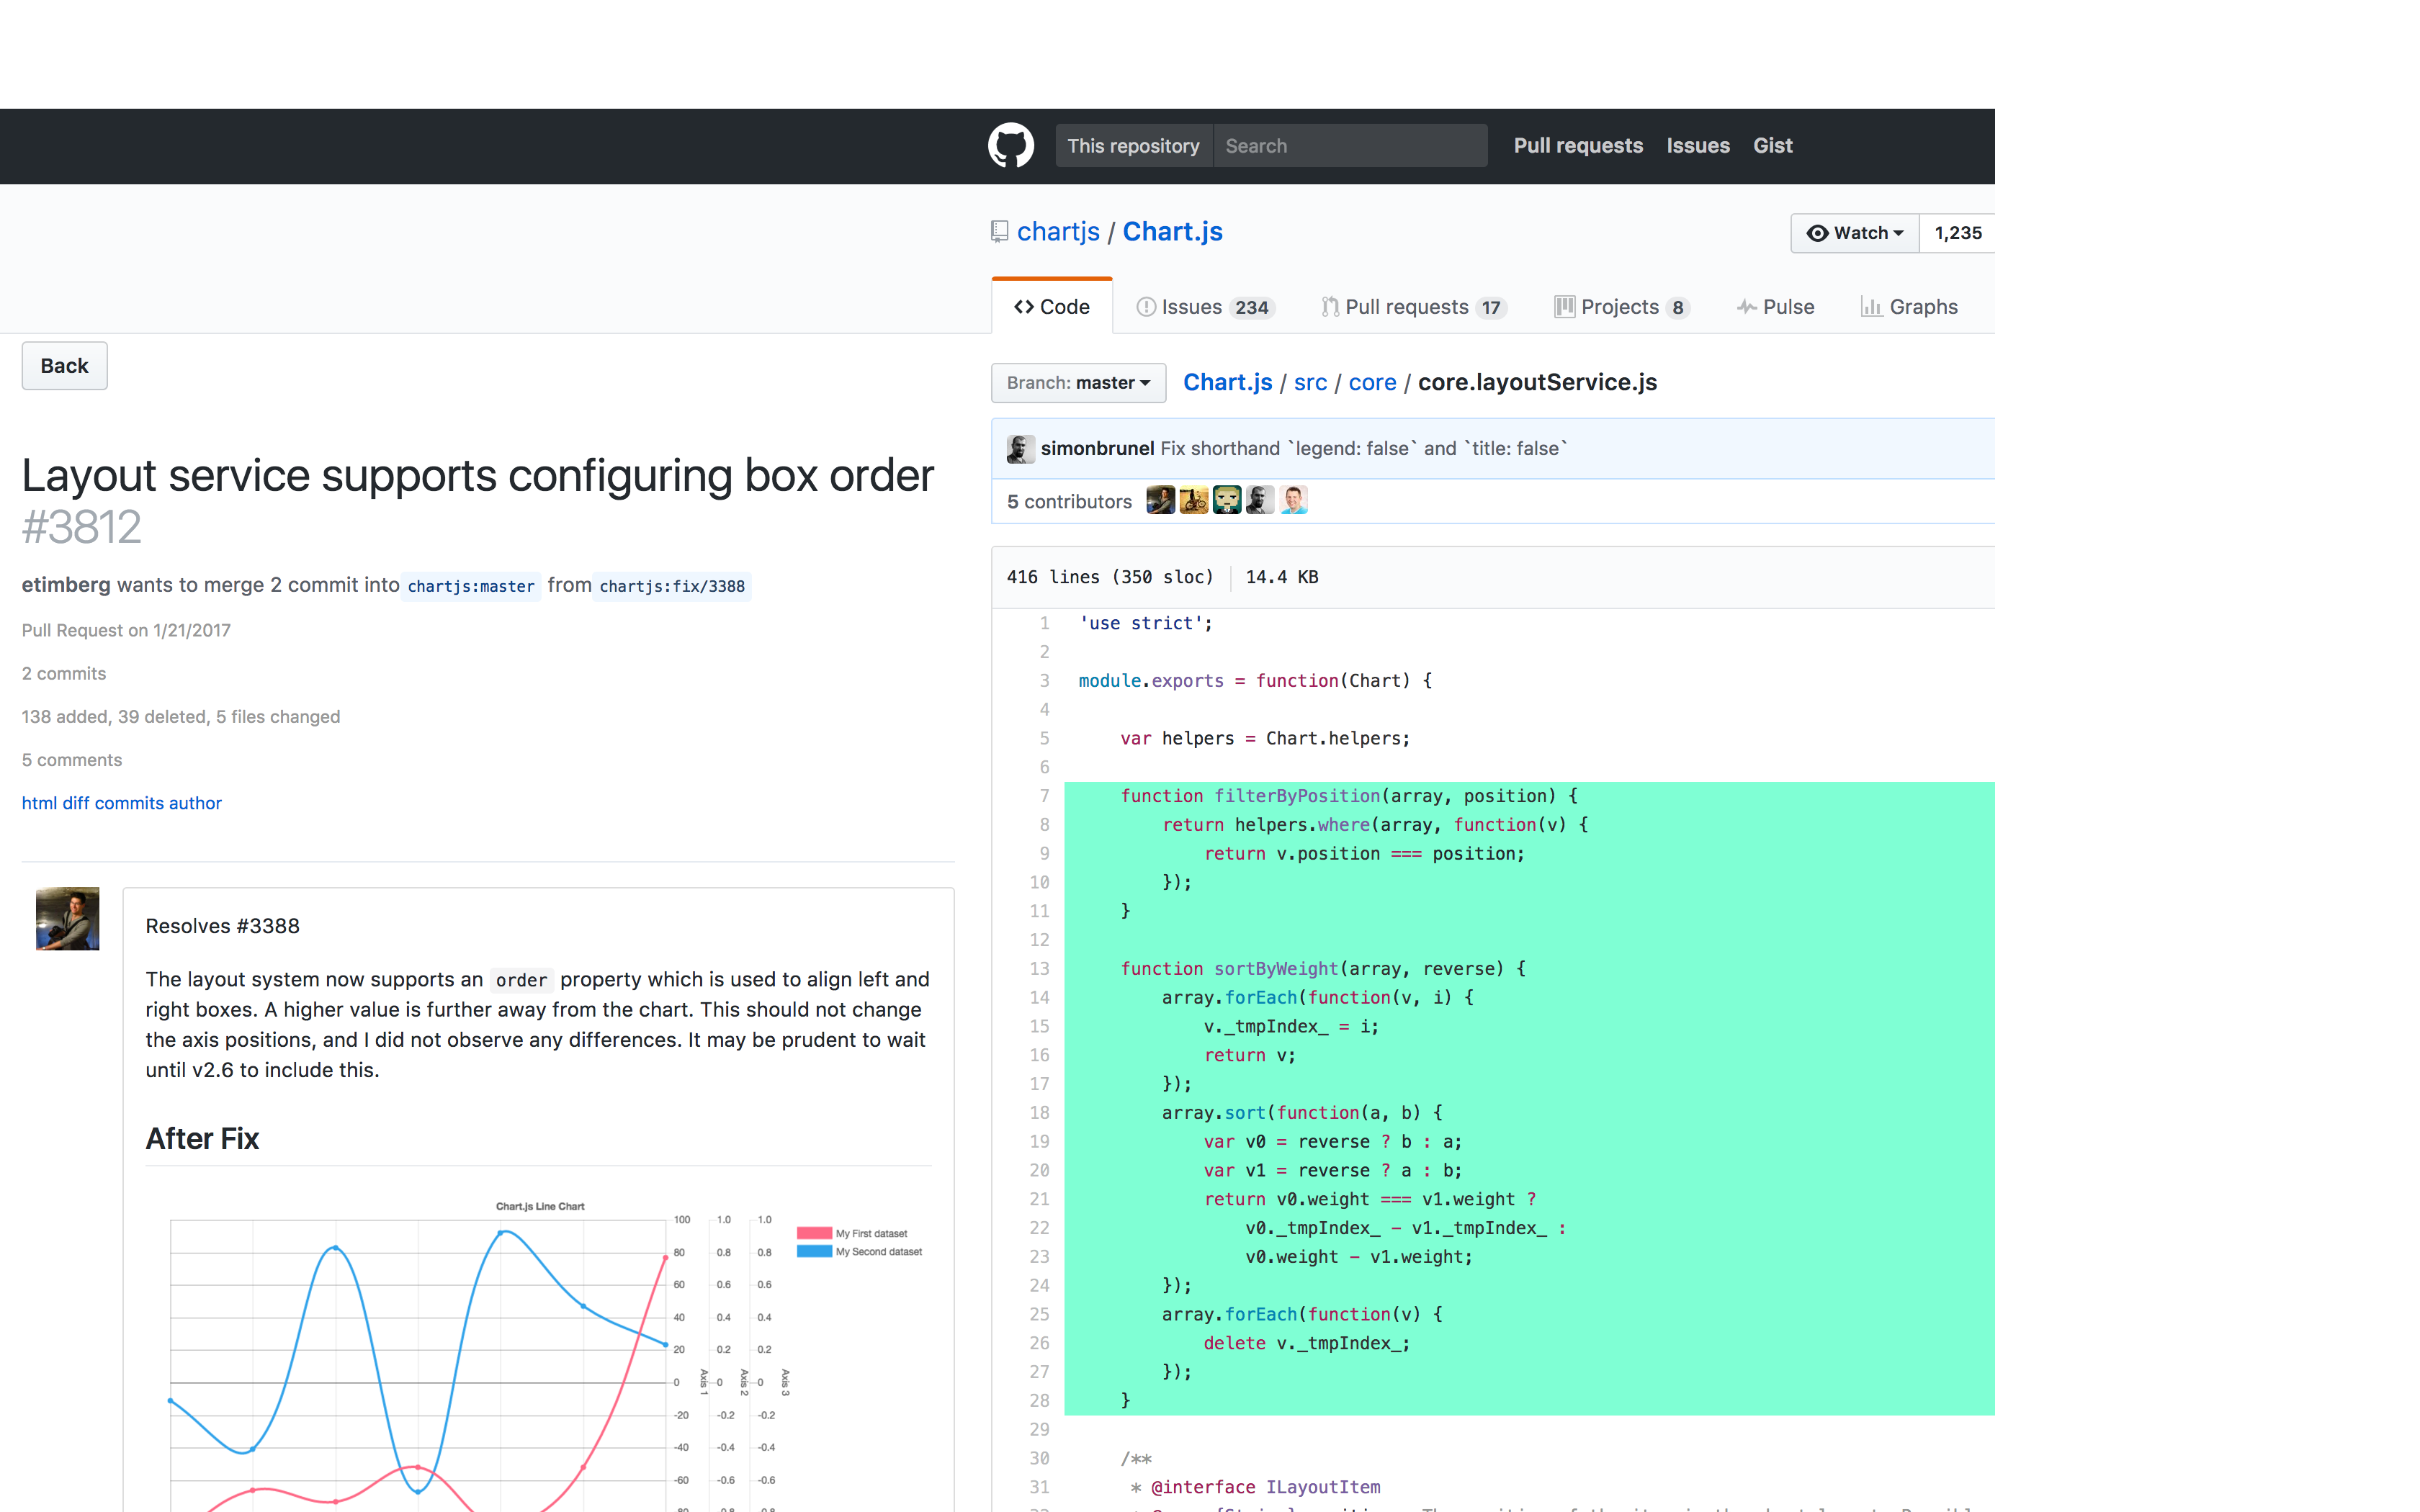
\includegraphics[width=1.2\columnwidth]{interface/top_image.png}
%   \caption{CodeGlass allows users to interactively examine descriptions and comments in pull requests relevant to the chosen portion of code (highlighted in light green). Information in these pull requests can be useful to understand development contexts.}~\label{fig:top}
%   \vspace{-8mm}
% \end{figure}

最近のソフトウェアプロジェクトでは、共同開発や分散開発をサポートするWebサービスであるGitHubが一般的に使用されています。
GitHubはプルリクエストを使ってソフトウェア開発を奨励しています。
プル要求は、コードの変更を説明と共に送信する方法です。
GitHubには、プルリクエストによるレビュープロセスを管理する機能もあります。
多くのプロジェクトではプル要求が積極的に使用されており、開発者はしばしばコード変更に関する詳細情報をそれらに含めます。
我々の形成研究は、プル要求がコード理解を容易にする有益な情報リソースとして役立つ可能性があることを見出した。
この見解は、コード片の理解をサポートするためのインタフェースをどのように設計できるかを検討する動機となる。

このホワイトペーパーでは、CodeGlassと呼ばれるインタラクティブなピースレベルのコード検査ツールを紹介します。
システムは、プルリクエストを抽出し、選択されたコードピースに関連するコメントをレビューする。
このようなやりとりを可能にするために、私たちのピースレベルの差分バックトラックアルゴリズムは、選択したコードピースに関連する過去のコミットとプルリクエストを識別します。
私たちの調査によると、CodeGlassは実装の根拠と開発履歴に関する情報を得るために参加者をサポートできることが明らかになりました。
この作品はヒューマン・コンピュータインタラクションとソフトウェア工学の分野に次の貢献をしています:

\begin{itemize}
\setlength{\parskip}{1mm}
\setlength{\itemsep}{0mm}
	\item 開発者が選択されたコードピースに関連付けられた過去のプルリクエストで説明を表示し、コメントを確認できるように、ピースレベルのコード検査をサポートするためのインターフェイス。
	\item ピースレベルの差分バックトラックアルゴリズムで、指定されたコード片の変更を含む一連のコミットを識別します。
	\item 定量的アルゴリズム評価は、我々のアルゴリズムがコード片の変化を高い精度で取り戻し、想起させることができることを示している。
    \item CodeGlassによるコードの理解と、プロフェッショナルな開発コンテキストでの潜在的なユースケースの改善されたパフォーマンスを明らかにするユーザー評価。
\end{itemize}




% %2
% \section{関連研究}
% 
コードを説明する情報を探す事はコード理解において重要かつ一般的な工程である~\cite{Program_comprehension_during_software_maintenance_and_evolution}。
ヒューマン・コンピュータ・インタラクションやソフトウェア工学の研究分野では、コードに関する情報の検索といったコード理解に必要な作業を様々な側面から支援する研究が行われてきた。
本章では、その中でも特に本研究と深く関係する3つの研究領域における先行研究について述べる。

\shibato{}{日本語でコロンってどう使うんだろうか}

\begin{itemize}
  \item コード変更の理解の支援
  \item ドキュメントの作成と活用の支援
  \item ソースコード及びプロジェクトの可視化
\end{itemize}


%%%%%%%%%%%%%%%%%%%%%%%%%%%%%
% Code comprehension involves seeking information to acquire knowledge about code ~\cite{Program_comprehension_during_software_maintenance_and_evolution}.
% Research in HCI and software engineering has explored ways to support various activities around code comprehension.
% We review three major research areas in code comprehension support closely relevant to our work: supporting code change understanding, creating and using documentation, and visualizing code and projects.


\subsection{コード変更の理解の支援}
% \subsection{Code Change Comprehension Support}
%diffやcommitの利用をサポートするようなシステムを入れる.

近年の多くのソフトウェア開発管理システムではコード差分を記録する事でコード変更を追跡する事が出来る。
加えて、開発管理システムの多くがバージョン管理のためにコミットの機能を提供している。
そういった開発管理システムにおけるコード変更や付随する説明文はコード理解において有益な情報を含んでいる。
そこで、先行研究ではコード変更に付随する情報を用いてコード理解を支援する手法が調査されてきた。

% Modern project management systems include the diff function by default, and enable code change tracking.
% They also introduce the notion of commits, used for version controls and code reviews.
% These code changes and related descriptions can contain helpful information to understand code.
% Prior research thus has examined approaches to supporting documentation and comprehension on code changes.

Bucknerら~\cite{JRipples}が開発したJRipplesは、コード変更がソースコード全体に対しどの程度影響を及ぼすかを理解することを支援する。
JRipplesはコード変更にバグが含まれていた場合、影響を受ける可能性があるクラスを提示する事が出来る。
Zhangら~\cite{Interactive_Code_Review_for_Systematic_Changes}はコード変更の理解を支援するCRITICSというシステムを開発した。
\shibato{CRITICSは与えられたコード変更と類似した過去のコード変更とそのレビューの記録を管理システムから検索する。}{double-check}
開発者はその記録を見る事で、コード変更の理解をより正確かつ効率的に行う事が出来る。
Buseら~\cite{Automatically_Documenting_Program_Changes}はコード変更のデータからその説明文を自動生成する手法を実装した。
彼らのユーザ評価では、自動生成された説明文は既存のログの89\%を代替可能である事が分かった。
同様に、 Linares-Vasquezら~\cite{ChangeScribe}が開発したChangeScribeもまた、コミットメッセージとして使用可能な説明文をコード変更から自動生成するシステムである。
コミットの内容や文脈を説明文に付与するために。ChangeScribeは複数の情報抽出アルゴリズムが実装されている。
しかし、彼らのシステム評価ではユーザの主観的な調査が行われていない。

% Buckner et al.~\cite{JRipples} presented JRipples that allows developers to understand how code changes can impact the rest of a project.
% The system shows classes which may have been impacted and developers can confirm if code changes cause any major issue.
% Zhang et al.~\cite{Interactive_Code_Review_for_Systematic_Changes} built a system, called CRITICS, to help developers understand code changes.
% Their system identifies similar code changes to the given diff.
% With the support of CRITICS, developers were able to conduct code review more efficiently and accurately.
% Buse et al.~\cite{Automatically_Documenting_Program_Changes} examined a method to automatically generate user-readable documentation from diff results.
% Their user study found that the auto-generated descriptions were sufficient to be replaced with 89\% of log messages.
% Similarly, ChangeScribe by Linares-Vasquez et al.~\cite{ChangeScribe} automatically creates descriptions which can be used as commit messages.
% Their system incorporates different information extraction methods to infer the content and contexts of commits~\cite{Using_stereotypes_to_help_characterize_commits,Automatically_capturing_source_code_context,Automatic_Generation_of_Release_Notes}.
% Their study, however, did not include subjective examinations on generated messages.


前述の先行研究とは異なり、本研究の目的はコード断片の理解を支援する事である。
コード変更に付随する情報はコード理解において有益である事が明らかとなっている~\cite{Commit_2.0, How_Do_Software_Engineers_Understand_Code_Changes}。
ChangeScribe~\cite{ChangeScribe}のようなシステムはコード変更の説明文の生成を支援する一方で、本研究にて開発するシステムではコード変更の説明文をコード理解に活用する事が目的である。

% Our primary focus is to support comprehension on a code portion none of which directly deals with.
% Prior work found that descriptions in commits are often useful to understand code changes~\cite{Commit_2.0, How_Do_Software_Engineers_Understand_Code_Changes}.
% A system like ChangeScribe~\cite{ChangeScribe} aims to support creating descriptions in commits whereas the main objective of this work is to utilize them as an information resource for code comprehension.



\subsection{ドキュメントの作成と活用の支援}
%APIのドキュメントなど,ドキュメンテーションを作ることとそれらを利用することサポートするようなものをここにいれる.

ドキュメントもまたコード理解における有用な情報源である。
ドキュメントの重要性は広く知られているが、ソフトウェア開発者には実際にはドキュメントを作成する時間や労力が不足している事が分かっている\cite{A_Study_of_the_Documentation_Essential_to_Software_Maintenance}。
そこでドキュメントの生成支援や既存のドキュメントを活用したコード理解の支援に関する研究が広く行われてきた。
Sridharaら~\cite{Automatically_Detecting_and_Describing_High_Level_Actions_Within_Methods}はJavaの関数の要約を自動生成するSWUMというシステムを実装した。
SWUMは\shibato{関数の言語的及びソースコードの構造的な関係性を解析し}{double-check}、ドキュメントとして使用可能な説明文を生成する事が出来る。
McBurneyとMcMillan~\cite{Automatic_Documentation_Generation_via_Source_Code_Summarization_of_Method_Context}らはSWUMをさらに改良し、与えられた関数が他のコードでどのように使われているかを生成する説明文に付与出来るようにした。
この手法により、自動生成される説明文に文脈を考慮した情報を追加する事が可能となった。
Stylosら~\cite{Jadeite}はJavaのAPIのドキュメントを同時に共同編集出来るJadeiteを開発した。
ユーザはJadeite上でドキュメントにエイリアスとなるクラス名や関数名を追加する事が出来る。
このエイリアスは実際のAPIと紐づいており、他のユーザはAPIの名前だけでなくそのエイリアスでもAPIを検索する事が可能となっている。

% Documentation is another main resource for code comprehension.
% Although the importance of documentation is well known, developers do not spare time and effort to create in practice~\cite{A_Study_of_the_Documentation_Essential_to_Software_Maintenance}.
% Research has examined various approaches to lowering the burden of creating documentation as well as utilizing information in existing documents.
% Sridhara et al.~\cite{Automatically_Detecting_and_Describing_High_Level_Actions_Within_Methods} developed a technique to automatically generate summary comments for Java methods.
% An algorithm in their system, called SWUM, can capture linguistic and structural relationships of keywords in code as well as count their occurrences.
% This enables richer textual descriptions about code that can be used in documentation.
% McBurney and McMillan~\cite{Automatic_Documentation_Generation_via_Source_Code_Summarization_of_Method_Context} further improved Sirdhara et al.'s approach by incorporating information about how methods are used in other parts of code.
% In this manner, they were able to include context information in auto-generated descriptions.
% Stylos et al.~\cite{Jadeite} presented Jadeite, which enables users to collaboratively edit Java API documentation.
% The system lets users annotate documentation with alias class or method names which they are expected to exist.
% These alias names, or placeholders, can be linked to existing APIs.
% They offer other developers multiple ways to reach to a desired API method.


既存のドキュメントをコード理解のために活用する先行研究も多く存在する。\shibato{}{in-situ をどう訳せばいいか分からない}
Subramanianら~\cite{Live_in_Documentation}はAPIとStack Overflow上のコード例を紐付けるアルゴリズムを実装した。
このアルゴリズムにより開発者は容易にAPIの使用例を確認することが出来る。
DekelとHerbslebが開発したeMoose~\cite{Improving_API_Documentation_Usability_with_Knowledge_Pushing}は、\shibato{ドキュメントから \XXX をコード理解のための重要な情報として抽出するシステムである。}{extracts imperative directives from documentation as important descriptions.}
ユーザ評価を行なった結果、eMooseを利用することでユーザはデバッグの成功率を改善することが可能となることが分かった。
TreudeとRobillardは、教師あり学習を用いてStack Overflowからドキュメントには含まれていない情報を抽出する手法を開発した。
彼らの行なったシステム評価では、教師なし学習を用いた手法と比較してより意味のある説明文をStack Overflowから抽出出来ることが明らかとなった。

% Research has also explored systems to encourage \textit{in-situ} use of existing documentation.
% Subramanian et al.~\cite{Live_in_Documentation} developed an algorithm to associate API methods with code examples available in Stack Overflow.
% In this manner, developers can easily access to actual examples of API use.
% Dekel and Herbsleb's eMoose~\cite{Improving_API_Documentation_Usability_with_Knowledge_Pushing}, extracts imperative directives from documentation as important descriptions.
% %attempts to solve an issue of an overwhelming amount of descriptions in documentation. Their system 
% A user study found that the presence of eMoose significantly improved a success rate of debugging tasks.
% Treude and Robillard~\cite{Augmenting_API_Documentation} used a supervised approach to extracting unseen information in API documentation from Stack Overflow.
% An evaluation confirmed that their method was able to extract more sentences that are meaningful and do not exist in API documentation than unsupervised approaches.

本研究はプルリクエストをコード理解のための情報源として活用することで、前述の先行研究をさらに補強するものである。
プルリクエストはGitHubを用いた開発では一般的に使用されており、プルリクエストの説明文はドキュメントとして活用出来る可能性がある。
本研究はCodeGlassの実装と評価を通じてプルリクエストの情報源としての可能性を調査する。
% This work complements the research above by utilizing pull requests as an information resource for code comprehension.
% Pull requests are a common practice in GitHub-based development, and their descriptions may serve as documentations.
% Our research uncovers such a potential through demonstrations of CodeGlass.



\subsection{ソースコード及びプロジェクトの可視化}
%コードやプロジェクトの推移を可視化するようなものをいれる.

先行研究では、ソースコードやプロジェクトの推移を可視化する手法についても広く調査されている。
Girbaら~\cite{How_developers_drive_software_evolution}は開発者がいつどのようにソースコードに変更を与えたのかを可視化するシステムを開発した。
Chronicler~\cite{Chronicler}はソースコードの推移を表すツリー状のグラフを通じて、ソースコードの過去の変更を\shibato{インタラクティブ}{日本語でなんて言うんだ、対話的?双方向的?}に調査することを支援するシステムである。
システム評価では、ユーザのタスクの成績に有意差は無かったものの、ツールを使用しない時と比較してChroniclerを使うことを好む実験参加者が多かった。
Bragdonら~\cite{Code_Bubbles}が開発したシステムは、コードを関数などの意味のある断片に分割し、バブル状にコード断片を可視化する事が出来る。
この可視化を使用する事でユーザは、目的の関数に到達するための時間とシステムの操作回数を削減する事が可能となる。
McMillan~\cite{Portfolio:_Finding_Relevant_Functions_and_Their_Usage}らはPortfolioという関数の定義と使用箇所を検索し特定するシステムを開発した。
Portfolioは関数とその呼び出しをネットワーク状に可視化する事が出来る。

% Researchers have also investigated interactive visualization to explore the context and usage of code.
% Girba et al.~\cite{How_developers_drive_software_evolution} developed Ownership Map visualization which illustrates when and how contributors have engaged in a project.
% Chronicler~\cite{Chronicler} allows developers to interactively examine the history of source code using Tree Flow visualization.
% Their user study participants preferred Chronicler to an interface without visualization though quantitative performance metrics did not show significant results.
% Bragdon et al.~\cite{Code_Bubbles} developed an interface which visualizes code by splitting into meaningful chunks (e.g., functions and methods) and showing them in separate bubble-like windows.
% Their visualization was helpful to reduce the completion time and the numbers of navigations and repeated interaction.
% McMillan et al.~\cite{Portfolio:_Finding_Relevant_Functions_and_Their_Usage} presented a code search system, called Portfolio, which supports users to find definitions and usage of functions.
% The system visualizes a network graph in which nodes and edges represent functions and their invocations, respectively.


上述の先行研究ではコード理解を目的としてソースコードやプロジェクトの可視化手法を調査している。
本研究においてもそれらの可視化手法を、まだ調査の対象にはなっていないプルリクエストの提示に応用する事が可能である。

% These projects suggest that code and project visualization can facilitate comprehension.
% Our work encourages future research on visualization techniques for pull requests which none of the projects above has examined.



% %3
% \section{Formative Studies}
% \label{section:Formative_Study}

\subsection{Interviews with Professional Programmers}
To be informed of the system design, we conducted a formative interview study with five professional programmers (PA1--5, all male).
Because it is already well known how important code comprehension is in general, our interview focused on how they attempted to develop understanding and what issues they encountered.
All participants regularly used GitHub in their work environments.
This part of the formative studies revealed the following two findings.
%Our interview study took approximately one hour.
%The participants were offered a compensation of approximately 15 USD in the local currency at the end of the interview.
%As we conducted our interviews in a local language, we translated quotes in English for the following report.

\subsubsection{Burden for Collecting Development Contexts}
% In collaborative development, understanding code written by others is crucial.
% However, effort for code comprehension can be substantial. 
% PA1 stated how tedious it can be when he was involved in code review.

% % \myquote{(コードレビューにおいて、人のコードを読む事は)まじめにやるとコード書くのと同じくらい時間かかるんですよ}{P1}
% \myquote{(In code review,) Understanding others' code can be as time-consuming as writing code if you do it seriously.}{PA1}

Code comprehension includes understanding the context of how the code has been developed in addition to what it executes.
PA1 mentioned a particular issue related to code review caused by the lack of context understanding.

% \myquote{プロダクトの背景がわからないことが課題となっていて、長く見ている人が初めてそのチーム内でレビューできるようになっていて、まだやっぱり新入りの人がコードレビューできるような状況までドキュメントが整備されていないし、やっぱり背景理解が難しい。}{P1}
\myquote{One issue is the lack of background knowledge about the product. It makes only old members able to perform code review. Documentation is not ready for new members yet so that they can perform code review. It is still difficult for them to understanding the background.}{PA1}

% This problem becomes more prominent when new team members were on board.
% P1 mentioned that he frequently observed that new team members struggled on collecting background information.

% % \myquote{やっぱりコードの背景というか、コンテキストがわからないので、そこはなんかわかんないのは当たり前だと思う}{P1}
% \myquote{It is unsurprising that new team members do not understand the project well because they do not know its context or background.}{P1}

Such development contexts can also be useful for existing team members as PA3 stated:

% \myquote{どういう背景があってこのコードを実装したのかが書いてあると嬉しい。}{P3}
\myquote{It would be great if it is clear why this code has been implemented.}{PA3}

% Software documentation is one of the best practices to share knowledge of source code among team developers.
% However, PA5 stated that creating documentation would cause additional overhead in a project, and his team decided not to engage in it.

% % \myquote{チーム内でもドキュメントを作ろうという流れになる事はあります、ありますけど、正直なところあのーそこにさけるパワーは今、ちょっと・・、開発スピードを重視したいので}{P5}
% \myquote{We do have plans to create documentation, but to be honest, we don't have bandwidth for it now. We want to focus on speeding up our development.}{PA5}

\subsubsection{Pull Requests as an Information Resource}
% Code review was a common activity we observed in our interviews.
% It is one development process where a developer validates code revisions developed by another programmer.
% Bacchelli and Bird~\cite{MotivationOfCodeReview-Bacchelli} reported that while the main motivation for code review was to identify defects, reviewers also expected additional benefits, such as learning alternative solutions or performing knowledge transfer.
% For these multi-faceted benefits, code review becomes an integral part of a modern development process.

% GitHub supports code review through pull requests.
% A pull request includes a description of revisions as well as the actual code changes.
% A reviewer performs merge (or pull in GitHub) when she finds the revisions to be bug-free and legitimate.
% Our participants mentioned that additional effort by developers can greatly facilitate a code review process.
% For instance, a well-written description of a pull request can offer a sufficient amount of information about and reasons for the code changes, supporting reviewers' activities.

Our interview participants regularly used pull requests in their project as part of a code review process.
They agreed that comments and logs in pull requests can be useful to obtain information about code. 
For instance, PA3 and PA5 commented that he often referred to past pull requests to understand implementation reasons.

% \myquote{それは、実装を見ててこれってどういう意図でこうなってんのとかが、気になった時は、結構プルリクエスト上で議論がなされていることが多いので、それを探しに行くことはあります。}{P3}
\myquote{When I have a question about why this implementation was made, I look for pull requests because they often include related discussions.}{PA3}

%\myquote{僕はわりと探っちゃうタイプなので、昔どういうことあったんだろうみたいなのはまあ追っちゃう感じですね。}{P5}

\myquote{I like digging into code, so I often look for pull requests to see what happened in the past.}{PA5}

% PA1 and PA3 stated that they and their team explicitly described contexts as well as the content of changes.


% % \myquote{重要だと思ってるのは、まあ一個一個何でどういう目的でやるのかっていうのを書くようにしてるんですよね、formatをwhyとwhatを書くようにしている}{P1}
% \myquote{What's important to me is to describe what each change does for what purposes. We have a format (for pull requests) to make sure to write why and what.}{PA1}
% % \myquote{見てもらう人のことは考えて、どういう変更をどういう意図で行ったのかっていうのは、書くようにしている}{P3}
% \myquote{I always think of the reader, and clearly write what changes I have made for what purposes.}{PA3}

% Similar to general code comprehension, understanding development contexts is important for code review.
% P4 mentioned that the problem arises when he asked external developers to perform code review. 

% %\myquote{他のチームにレビューを頼む時に、プロダクトの背景がわからないことが課題となっていて、長く見ている人が初めてそのチーム内でレビューできるようになっていて、まだやっぱり新入りの人がコードレビューできるような状況までドキュメントが整備されていないし、やっぱり背景理解が難しい。}{P4}

% \myquote{When I have to ask someone in another team to review, the problem is that he does not have background knowledge about the project. People cannot do proper reviews until they are in a team for a long time.}{P4}

\subsection{Lab Study on Existing Command-based Approaches}

%Our interview with professional programmers revealed that past pull requests can be a useful resource for understanding code.
We conducted another formative study in our laboratory to understand how existing tools can support extraction of past pull requests.
%%%%%%%%%
% WWWWWWWWHYYYYYYYYYYYYYYYYYYY
% Specifically, we looked into tig\footnote{\url{https://github.com/jonas/tig}} and recursive-blame\footnote{\url{https://github.com/scottgonzalez/recursive-blame}}.
%%%%%%%%%%%%
To understand how these tools would be useful even for novice developers, we recruited seven university students (PB1 -- PB7) who had sufficient experience in GitHub and pull-request-based development.
We asked the participants to find pull requests related to portions of code in Chart.js given by the experimenter using tig and recursive-blame.
We then conducted a short interview to understand the user experience of these tools.


\subsubsection{Limited commit backtracking capability}

% P1 stated that recursive-blame often cannot trace back the history when the specified pattern of code was changed.

% % \myquoute{単純に名前が変わったりすると追えないとかがあるから、基本的にある程度あいまい検索ができるといいんだと思う}{P1}

% Tig finds the latest commit and version containing a change on the user-selected line of code using the git-blame command.
% However, it may fail to determine the commit when changes are substantial as P6 stated:

% \myquote{色々書きかえると結構すぐ追えなくなりますよね}{P6}

%The tools tested only take constrained input for search (a line of code and a regular expression or keyword in tig and recursive-blame, respectively).
%This limitation prevented our participants from correctly identifying relevant pull requests.
Our participants pointed out that existing tools cannot clearly inform whether the portion of interest was completely deleted or moved to a different part (e.g., by refactoring).
This is because the tools only show the deletion of such a portion and manual confirmation is necessary.

% \myquoute{違う名前や使い方が変わったときに、じゃあ何になったんだろうというってのを探すためには、前の名前しか知らないときは自分で探さないといけない。削除なのか、変更なのかわからないのが今のツールではわからない。}{P4}
\myquote{For example, when I found revisions on names or usage, I have to eyeball to figure out whether deletion or changes had occurred, which  these tools cannot tell me.}{P4}


\subsubsection{Limited interaction}
Although the two tools can identify past pull requests, their interfaces do not offer an overview of descriptions and comments.
This diminishes the utility of the tools as code comprehension support.
One of our participants commented that an overview of relevant pull requests would be desirable.

% \myquoute{全部やった後にさ、descriptionなかったらさ、なんやねーんって感じやん。多分descriptionが一番大事だから、はずれだったらすぐ次のを見せてほしい}{P2}
\myquote{I think descriptions are the most important. So I want to have a way to quickly move on to the next if the current pull request isn't useful.}{PB2}

% \myquoute{一度にいくつか(プルリクエストを)見られればうれしいかなと思う、まとめて勝手に深追いしてほしい}{P4}
\myquote{If I can see multiple pull requests at one time, that would be great. A system should just track back automatically.}{PB4}

%P5 wanted a system that simultaneously provides code and description in pull requests.
% \myquoute{コードと説明文の二つを同時に表示してあげるインタフェースがあると、使いやすいインターフェースかなと思うしとっつきやすいかなと思う}{P5}

Tig and recursive-blame take a single line of code and a regular expression or keyword for search, respectively.
Our participants complained that this search method does not fit to their expected use cases, and  the tools should support selection of multiple lines or code pieces.

% \myquoute{コード読んでて、この行だけわかんないってなることはないから}{P1}
\myquote{It's unlikely that I do not understand only this particular line when I read code.}{PB1}

% \myquoute{このifの中みたいな、意味のある単位で見たい。ifの行自体は別にそれほど興味ないし中身が大事かなみたいな}{P5}
\myquote{I want to look into a meaningful chunk, such as code inside this if block. I am not really interested in the line of the if statement itself.}{PB5}

%\subsubsection{Limited search capability}
% \myquoute{キーワードで検索は面倒というか、自分が思ったところを検索出来ているのか不安。どこが引っかかるか直感的じゃないから、tigのほうがいいかも}{P3}




\subsection{Summary}
Our interview studies highlight the following findings.

\begin{enumerate}
\setlength{\parskip}{1mm}
\setlength{\itemsep}{0mm}
%\item Developers are frequently required to understand codes before performing further actions (e.g., reviewing and making revisions).
\item Developers desire to obtain relevant information about the portion of code they are investigating for understanding, but they do not always have appropriate support.
\item Past pull requests can be useful to understand the context or reasons of code changes.
\item Existing tools, such as tig and recursive-blame, have limited capabilities on backtracking and interaction. In particular, existing methods would not work well for changes that involve relocation.
\end{enumerate}

These findings lead us to a hypothesis that supporting examination with past pull requests would be helpful to support comprehension of code portions though existing approaches are not easy to use.


% 		\begin{figure*}
%         \centering
%             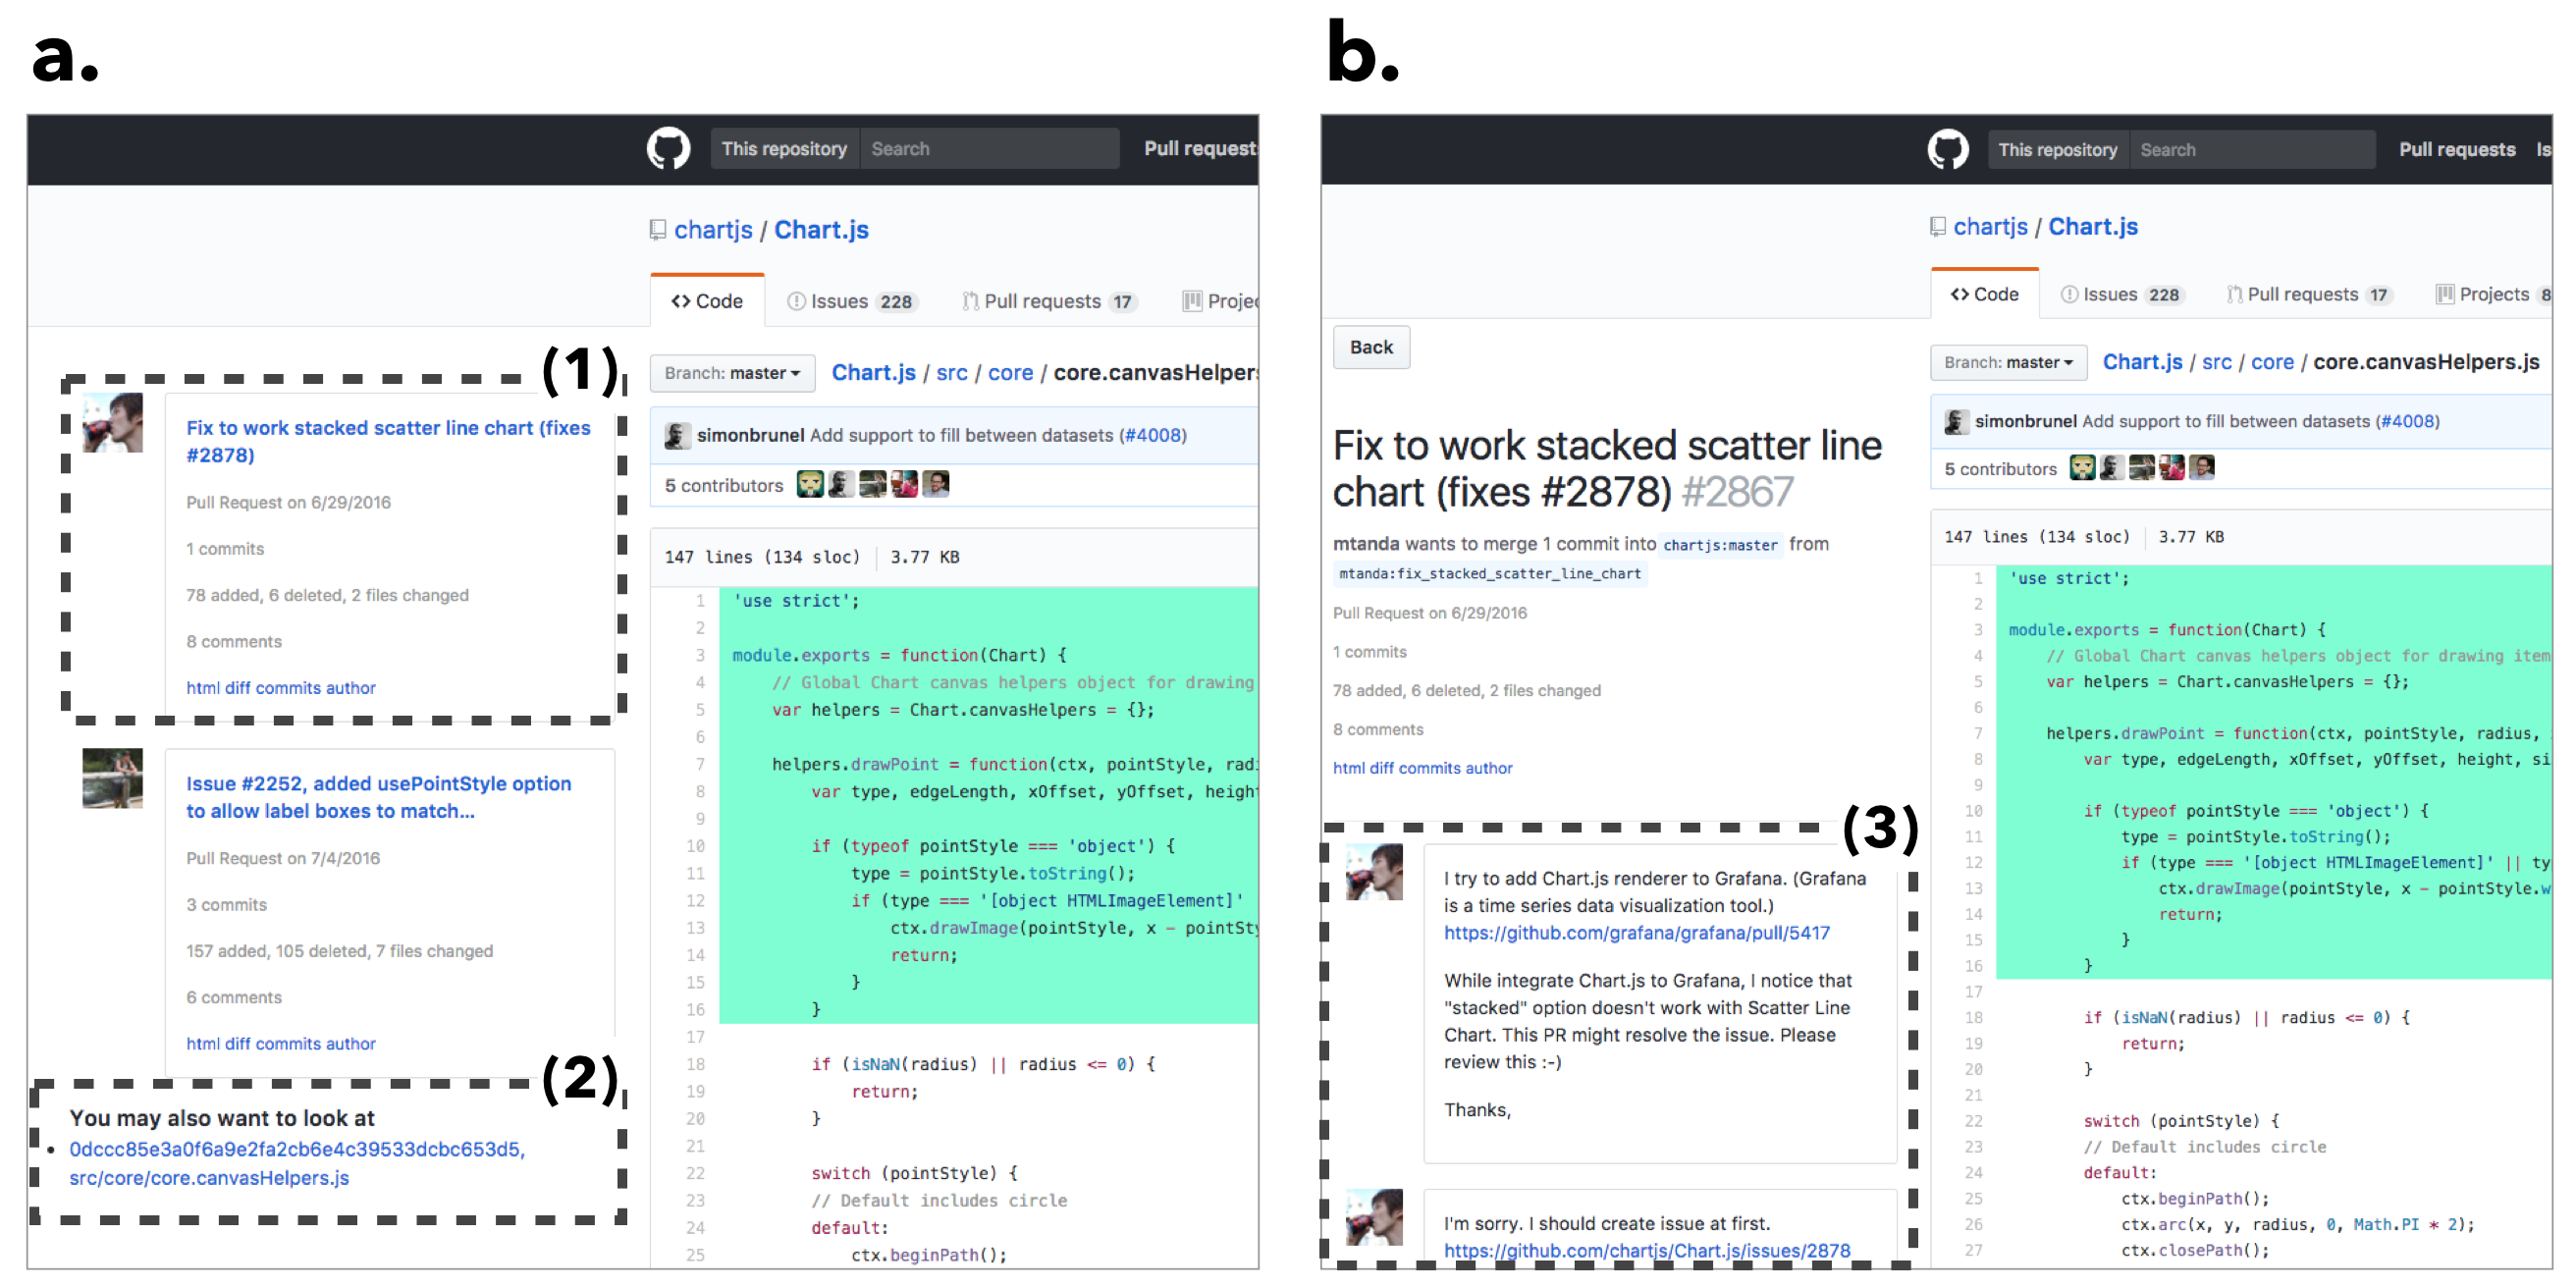
\includegraphics[width=2.0\columnwidth]{interface/CodeGlass.png}
%             \caption{The CodeGlass interface displays a series of pull requests associated with the selected code piece (highlighted in light green) in the chronological order. (1) Each pull request is summarized in a separate box. A summary shows the title of a pull request, its ID, and the numbers of commits, lines and files changed, and comments as well as links for additional information. (2) CodeGlass also suggests commits that are not included above but can be relevant if there exists any. When clicking one of them, the user can view the version associated with the selected commit and further investigate how code has been developed. (3) When the user clicks the title, CodeGlass presents review comments in the selected pull request.}~\label{fig:WebInterface}
%             \vspace{-5mm}
%       \end{figure*}
      
      
      
      

     


% %4
% \section{Interactive Piece-level Code Examination}
% We develop an interactive piece-level code examination tool, called CodeGlass.
A code piece is defined as any of consecutive lines in code.
It can be a single line, function, class or even the entire code in a file.
CodeGlass extracts the revision history on the selected code piece from commit logs.
Its interface then provides an overview that shows past pull requests associated with the selected code piece which contain descriptions, commits, and review comments.


CodeGlass also allows developers to examine past pull requests and commits on any line of code, not limited to meaningful chunks (e.g., classes or functions).
This capability is useful when developers need to investigate large classes and functions because they can have freedom to break down into smaller portions for their examination.

% GitHub displays a source code in a file in the red frame in Figure~\ref{fig:WebInterface}.
% CodeGlass provides ``Fetch'' button~(i.e., blue frame in Fig.~\ref{fig:WebInterface}) and a feature that the user can select codes by pointer~(i.e., green frame in Fig.~\ref{fig:WebInterface}).
Figure~\ref{fig:WebInterface} shows the CodeGlass interface.
The user specifies a code piece on which she desires to read descriptions and review comments of past pull requests simply by a mouse drag~(highlighted in light green in Figure~\ref{fig:WebInterface}).
CodeGlass displays a series of relevant pull requests in the chronological order as shown in Figure~\ref{fig:WebInterface}a.
Each pull request is summarized in a separate box ((1) in Figure~\ref{fig:WebInterface}a).
Each summary includes the title of a pull request, its ID, and the numbers of commits, lines and files changed, and comments.
It also contains links to the original pull request page, the diff summary, review comments, and the author's page with which users can further investigate details.
In addition, CodeGlass can also suggest other potentially-relevant commits if there exists any ((2) in Figure~\ref{fig:WebInterface}a).
When clicking one of them, the user can view the version associated with the selected commit and further investigate how code has been developed.
When the user clicks the title of a pull request summary, CodeGlass presents its review comments ((3) in Figure~\ref{fig:WebInterface}b).

      
The current CodeGlass system takes a server-client implementation.
The CodeGlass interface is implemented as a Google Chrome extension.
When the user selects a code piece, the interface sends the repository name, file name, and line numbers of the selected code piece to the server.
The server then estimates how the given code piece has been changed with the DiffTrack algorithm (explained later).
It extracts commits in which the selected code piece had revisions. 
The server then obtains pull requests containing these commits through GitHub API, and sends them back to the interface.

Our current prototype would function for any public repository on GitHub because the backend algorithm is language-agnostic as we explain later.
With proper permission settings, CodeGlass would be available even for private repositories.
% There are 57 million active repositories as of April 2017\footnote{\url{https://github.com/blog/2345-celebrating-nine-years-of-\\github-with-an-anniversary-sale}}.



% %5
% \section{Piece-level Diff Backtrack Algorithm}
% \label{section:Piece_level_Diff_Backtrack_Algorithm}

The CodeGlass server system needs to obtain commits that involve changes on the code piece selected by the user.
Such an algorithm needs to locate the portion in a past commit which best matches with the given code piece.
To make CodeGlass viable in realistic use, we have the following design considerations for the algorithm.

%       \begin{figure}[!t]
%         \centering
%             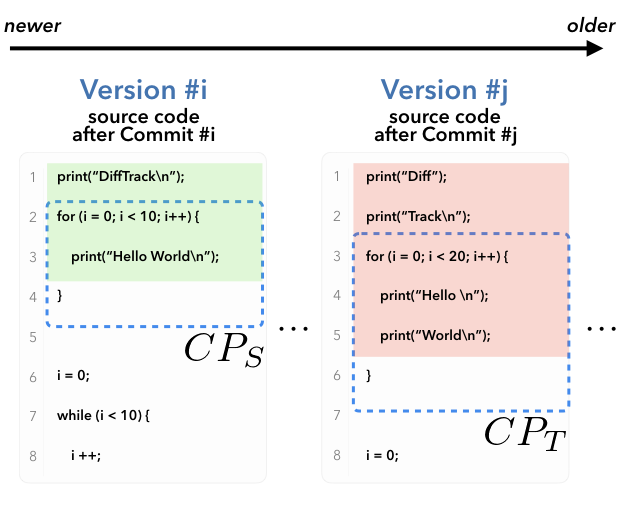
\includegraphics[width=0.9\columnwidth]{algorithm/limitation.png}
%             \caption{An example illustration of a source and true target code piece ($CP_{S}$ and $CP_{T}$). In this and following figures, red and green lines represent deleted and added lines between two versions (\#$i$ and \#$j$, $i>j$), respectively. A code piece in the newer version serves as $CP_S$ (lines in the broken frame in Version \#i). A backtrack algorithm estimates the location of $CP_{T}$ given $CP_{S}$, and runs iteratively with older commits. An estimated target code piece is denoted as $\widehat{CP_{T}}$. The ideal $\widehat{CP_{T}}$ is $CP_{T}$. This backtracking returns a series of commits associated with the code piece originally selected by the user.}

% 			\label{fig:CommitHistory}
%       \end{figure}
      
\begin{itemize}
\setlength{\parskip}{1mm}
\setlength{\leftskip}{7mm}
\setlength{\itemsep}{0cm}
\item[DC-1.] Accurately identify the location of a code piece in an older version even if changes occurred within it.
%\item[DC-2.] Run in real time regardless of the project scale and code length as well as the size of a code piece.
\item[DC-2.] Be compatible with any type of program-related files including style sheets and configuration files.
\item[DC-3.] Perform at a line-level granularity, from a single line to the entire file, to support unconstrained interaction.
\end{itemize}



      

Before explaining the details of our algorithm, we define a source and target code piece.
A source code piece ($CP_{S}$) means a code piece in a commit.
Using $CP_{S}$, the DiffTrack algorithm estimates a target code piece in an older commit.
We denote a true and estimated target code piece as $CP_{T}$ and $\widehat{CP_{T}}$, respectively.
Ideally, $\widehat{CP_{T}}$ is exactly the same set of lines of $CP_{T}$.
As the DiffTrack algorithm is executed iteratively, an additional subscript $i$ represents a code piece in the $i$-th version from the initial commit (i.e., $CP_{Si}$ is the source code piece in Version \#$i$).
We assume that the number of $CP_T$ is always one.

%The iteration occurs by using a target code piece as the source in the next step (i.e., $CP_{Sj} = \widehat{CP_{Ti}}$, $i>j \geq 1$).

\subsection{Limitations with git and git-blame commands}
\label{subsection:Limitations_with_git_commands}


%     \begin{figure}[tb]
%             \centering
%           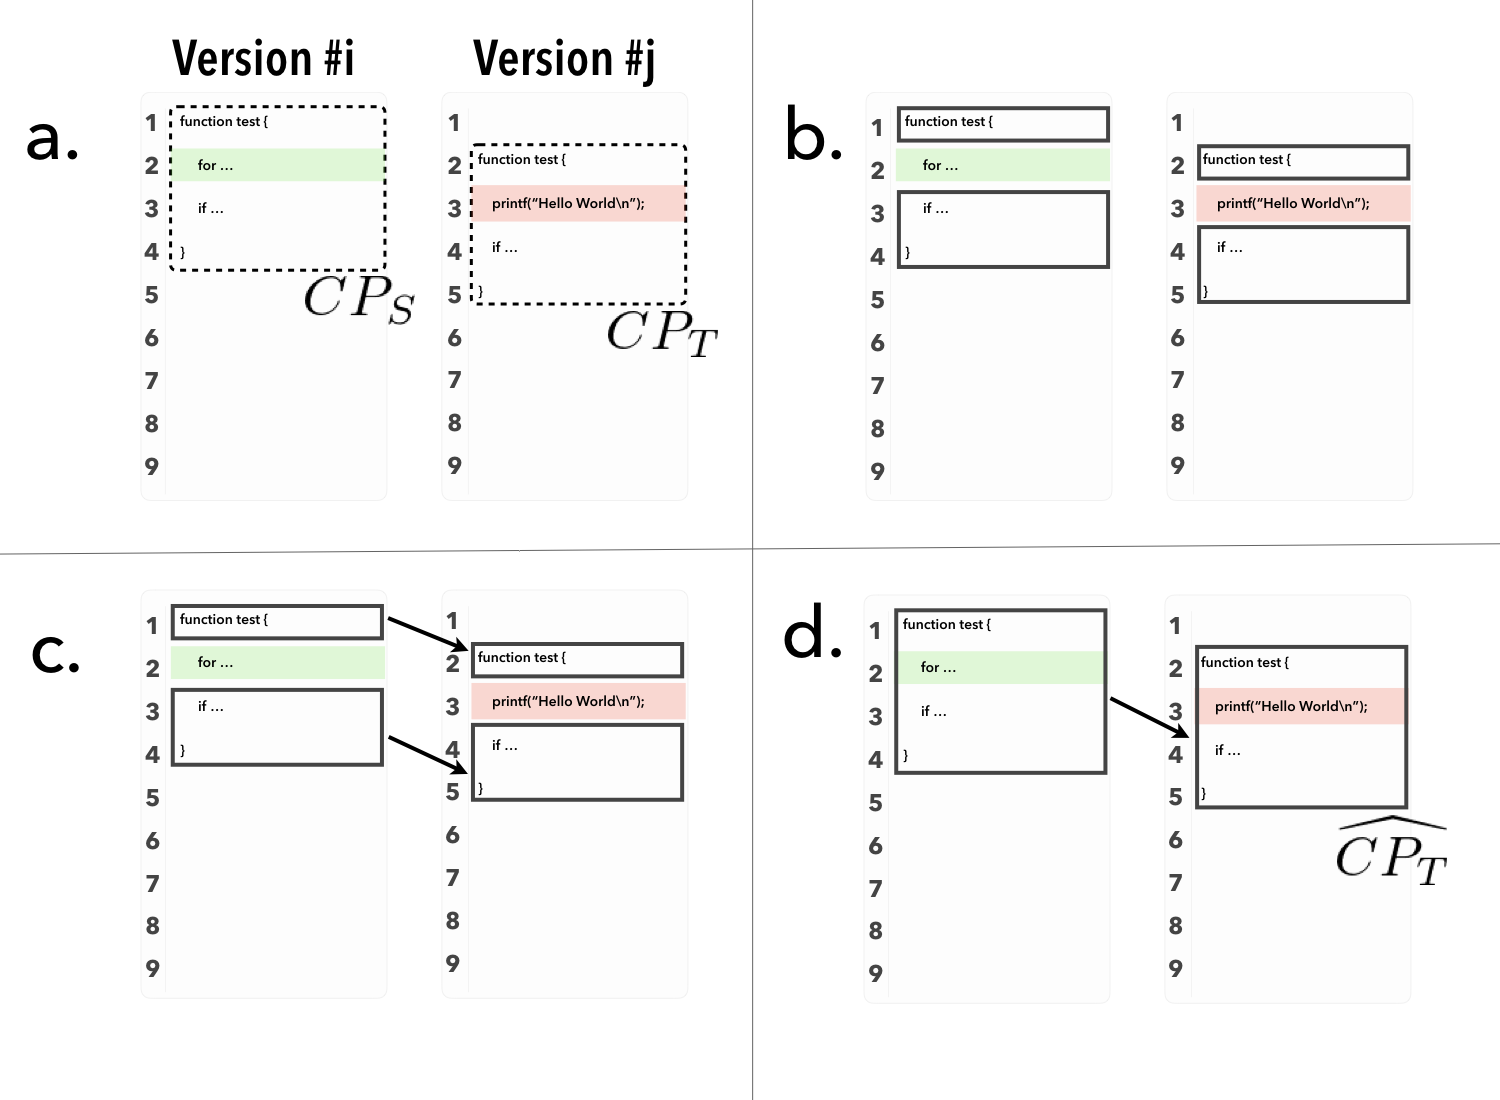
\includegraphics[width=1.0\columnwidth]{algorithm/Cases_001.png}
%           \caption{Case A: $CP_S$ includes unchanged lines that enclose the revised portion. (a) $CP_S$ and $CP_T$ are line 1--4 in the source commit and line 2--5 in the target commit, respectively. (b) The unchanged lines in $CP_S$ enclose the revised portion. (c) The unchanged lines serve as an anchor for search. (d) DiffTrack thus immediately determines line 2--5 as $\widehat{CP_T}$.}
%           \label{fig:caseA}
%     \vspace{-2mm}
%     \end{figure}


%     \begin{figure}
%       \centering
%         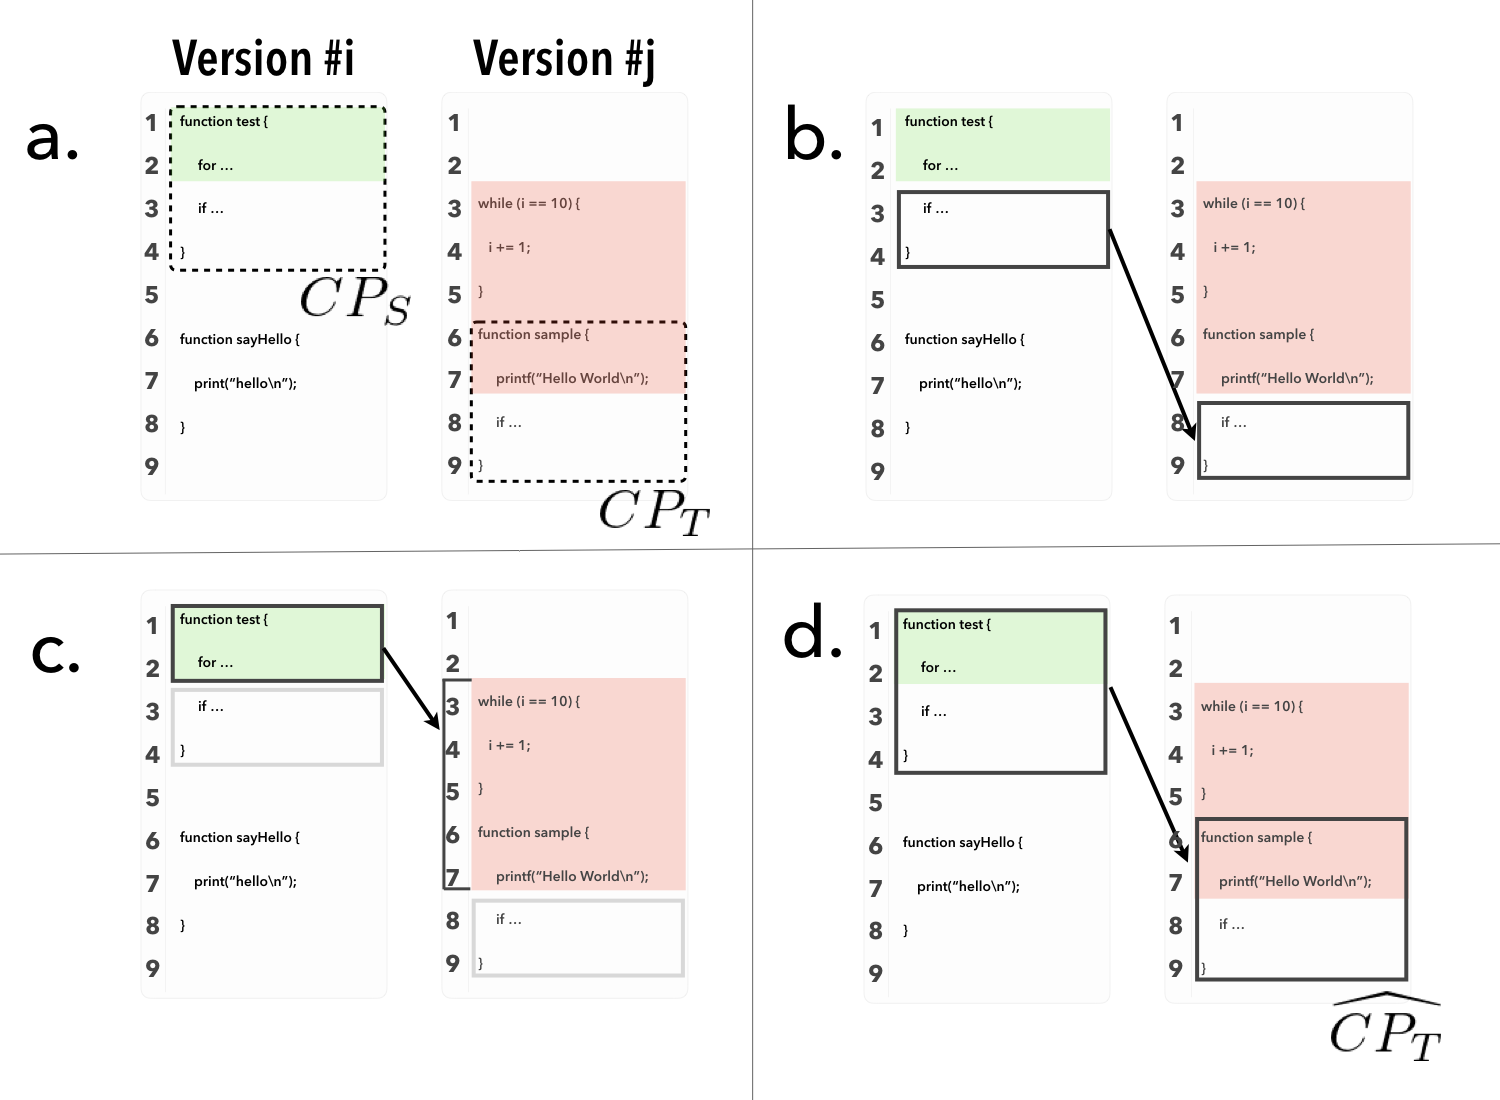
\includegraphics[width=1.0\columnwidth]{algorithm/Cases_002.png}
%         \caption{Case B: $CP_S$ includes unchanged lines that do not enclose the revised portion. (a) $CP_S$ and $CP_T$ are line 1--4 in the source commit and line 6--9 in the target commit, respectively. (b) DiffTrack first performs matching with the unchanged lines. (c) It removes unchanged lines (line 1 and 2) in the target commit from the search space. (d) It then performs fuzzy string search matching to identify lines most similar to the revised lines in the source commit. It finally determines line 6--9 $\widehat{CP_T}$.}~\label{fig:caseB}
%     \vspace{-5mm}
%     \end{figure}


Figure~\ref{fig:CommitHistory} shows an example of code changes between two versions (\#$i$ and \#$j$, $i > j$).
Suppose that our system needs to identify commits related to line 2--4 in Version \#$i$ to extract associated pull requests.
Thus, this portion is $CP_{Si}$~(the broken frame in Version \#$i$ in Figure~\ref{fig:CommitHistory}).
The git-blame command can point to the latest commit in which any part of $CP_{Si}$ was affected.
Thus, it is straightforward to find Commit \#$j$.
However, it provides \textit{only} the latest commit that contains changes in $CP_{Si}$.
This means that a system needs to find $CP_{Sj}$ (or $CP_{Ti}$) given $CP_{Si}$ to trace back to older commits and iteratively perform git-blame.
However, a diff log merely contains a set of line additions and deletions, which do not directly represent which revised lines are related to $CP_{Si}$.
In other words, git-blame cannot immediately provide the location of $CP_{Ti}$.
% In the example of Figure~\ref{fig:CommitHistory}, a system can only know that there are three lines of additions and five lines of deletions.
% But it is not immediately clear which revised lines are related to $CP_{Si}$, and we thus need a method to estimate the location of $CP_{Ti}$ (which also serves as $CP_{Sj}$ for further backtracking).

\subsection{Limitations with abstract syntax trees}

Another alternative approach is to use fine-grained source code change extraction methods~\cite{GumTree, Change_Distilling}.
These approaches can extract not only additions or deletions but also infer syntactic changes, such as updates or moves.
They use an abstract syntax tree (AST) to compute similarity between the two versions and extract syntactic changes.
%One example of such algorithms is Change Distiller developed by Fluri et al~\cite{Change_Distilling}.
%Falleri et al.'s GumTree~\cite{GumTree} further improve precisions on detecting code moves.
Although these algorithms are designed to compare multiple versions of an entire source code file, it is theoretically possible to implement them to perform matching of code pieces.


Nevertheless, we decided not to consider AST-based methods because they do not satisfy DC-2 and 3 in general.
As methods using abstract syntax trees require a parser, additional configuration is necessary for adaptation to different programming languages.
For example, GumTree~\cite{GumTree} is only compatible with C, Java, JavaScript, and Ruby as of April 2017.
Internal parsing can lead to large computational overhead for long code pieces.
In addition, a selected code piece should be syntactically correct, which also limits user experience.
We thus developed an algorithm called DiffTrack.

\subsection{DiffTrack Algorithm}

The DiffTrack algorithm can identify a set of commits that contain changes on a user-selected code piece.
It first finds the latest commit and version containing changes on the code piece by the git-blame command.
The algorithm then locates a portion of code in this version which is the most similar with the given code piece.
It then performs this operation iteratively by using the estimated portion of code as the next source code piece to trace back to even older versions.
For instance, in the example of Figure~\ref{fig:CommitHistory}, the estimated code piece (i.e., $\widehat{CP_{Ti}}$) given $CP_{Si}$ becomes $CP_{Sj}$.
The algorithm stops when it reaches to the oldest version or no reasonable $\widehat{CP_{T}}$ is found.
This process results in a set of commits containing changes on the code piece the user initially selects.
It finally extracts pull requests that include these commits and returns them to a client.
CodeGlass ultimately visualizes the pull requests in its interface.
In this section, we explain the behavior of DiffTrack with three cases in all of which $CP_{S}$ includes revisions.


\subsubsection{Case A: $CP_S$ includes unchanged lines that enclose the revised portion.}


$CP_S$ contains revised lines between the unchanged portions (i.e., line 2 in Version \#i in Figure~\ref{fig:caseA}).
In this case, the algorithm first uses the unchanged lines (line 1, 3, and 4) as an anchor to find $\widehat{CP_T}$.
In addition, only changed lines should be included between the unchanged portions.
The algorithm, therefore, immediately identifies $\widehat{CP_T}$ as the unchanged portions and changed lines in-between (i.e., line 2--5 in Version \#$j$).

\subsubsection{Case B: $CP_S$ includes unchanged lines that do not enclose the revised portion.}

%     \begin{figure}[tbp]
%             \centering
%           \includegraphics[clip, width=8cm]{algorithm/CaseB.png}
%           \caption{An example of case B (where $CP_S$ includes unchanged lines that do not enclose the revised portion).
%           $CP_S$ and $CP_T$ are from line 1 to 4 in the source commit and from line 6 to 9 in the target commit, respectively.~(a)
%           The algorithm first perform matching with the unchanged lines.
%           In this example, codes from line 3 to 4 in the source commit matches with counterparts from line 8 to 9 in the target commit.~(b)
%           The algorithm removed unchanged lines from the target commit (i.e., line from 1 to 2 in the target commit) to prune the search space.~(c)
%           It then performs fuzzy string search matching to identify codes most similar to the revised lines~(i.e., line 1 and 2 in the source commit).
%           The algorithm finally determines from line 6 to 9 in the target commit as $CP_T$.~(d)
%           }
%           \label{fig:caseB}
%     \end{figure}
    

$CP_S$ contains unchanged lines, but the revised portion is not enclosed.
Figure \ref{fig:caseB} presents such an example where the first half has been revised while the other stays unchanged.
   
Similar to the previous case, the algorithm first performs matching with the unchanged lines.
This matching result narrows down the possible lines for $\widehat{CP_T}$ (above line 7 in this example).
The algorithm further reduces the search space by removing remaining unchanged lines because it can assume that the rest of $\widehat{CP_T}$ should be revised lines.
In this example, line 1 and 2 are unchanged, and thus they are removed from the search.
The algorithm then performs fuzzy string matching between the revisions (explained in detail later), and identifies the set of lines with the highest similarity score (line 6 and 7 in this example).
DiffTrack determines line 6--9 as $\widehat{CP_T}$.


\subsubsection{Case C: $CP_S$ does not include unchanged lines.}

%     \begin{figure}[tbp]
%             \centering
%           \includegraphics[clip, width=8cm]{algorithm/CaseC.png}
%           \caption{An example of case C (where $CP_S$ does not include unchanged lines).
%           $CP_S$ and $CP_T$ are from line 1 to 3 in the source commit and from line 5 to 7 in the target commit, respectively.~(a)
%           The algorithm first removes all unchanged lines from the target commit.~(b)
%            It then performs fuzzy string matching on all possible string chunks, and finds the most similar match.~(c)
%            The algorithm finally determines codes from line 5 to 7 in the target commit as $CP_T$.~(d)}
%           \label{fig:caseC}
%     \end{figure}
    
% \begin{figure}
%     \centering
%       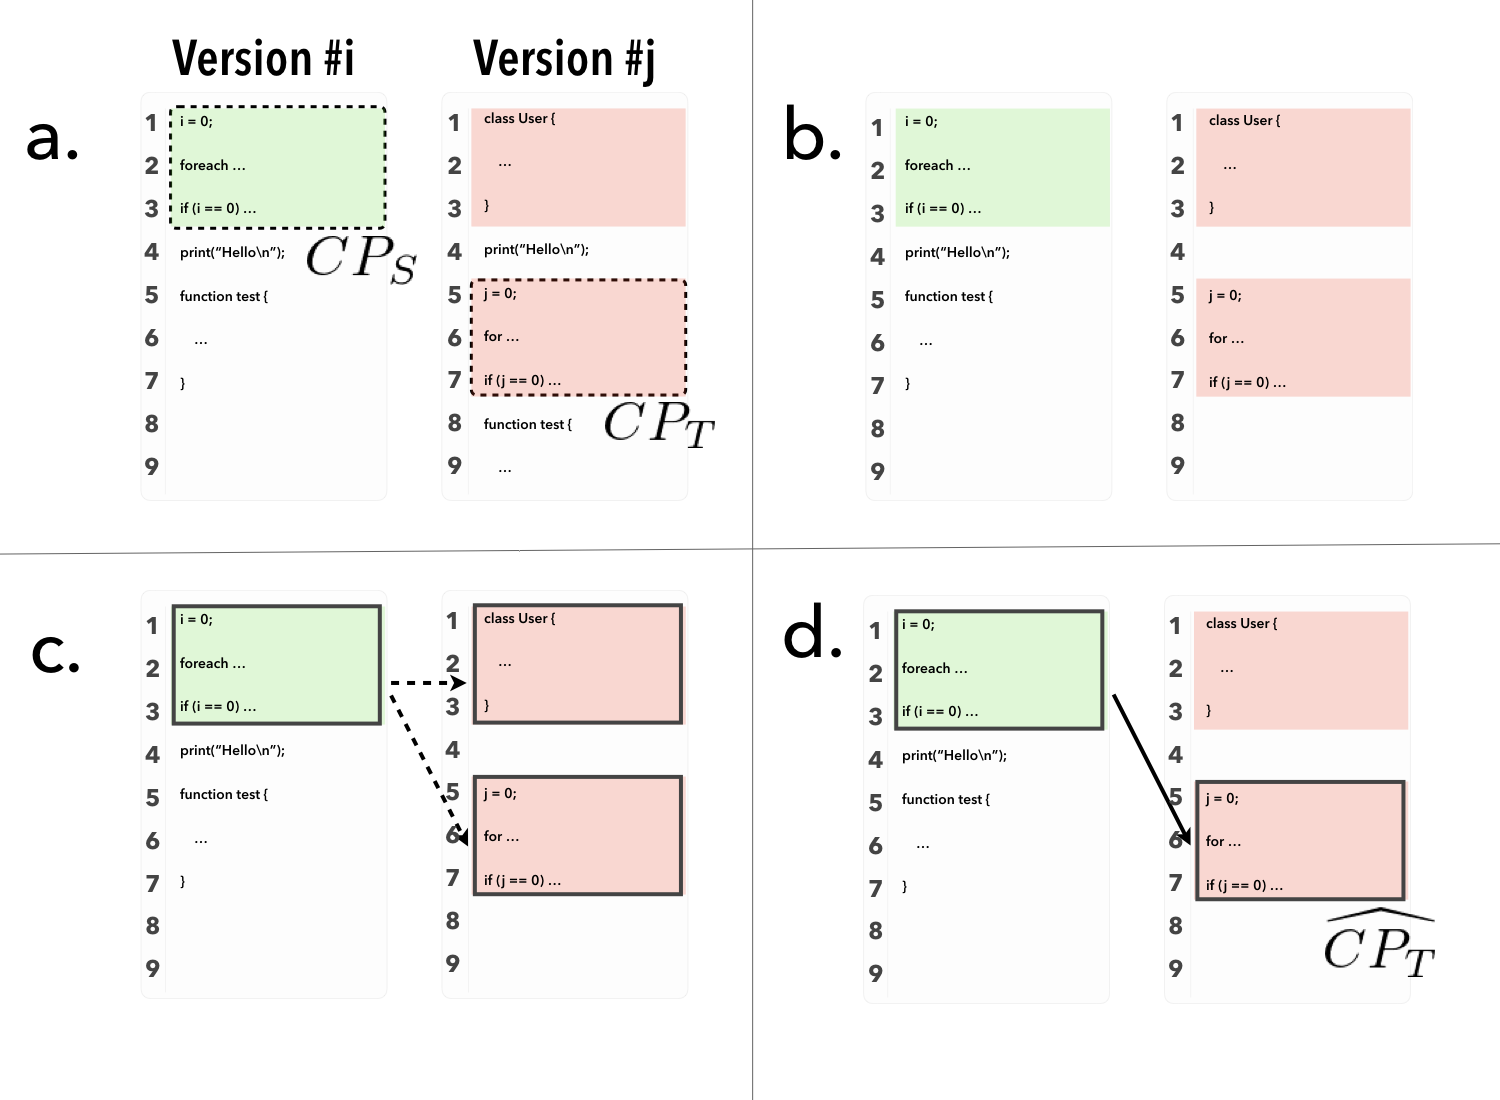
\includegraphics[width=1.0\columnwidth]{algorithm/Cases_003.png}
%       \caption{Case C: $CP_S$ does not include unchanged lines (a) $CP_S$ and $CP_T$ are line 1--3 in the source commit and from line 5--7 in the target commit, respectively. (b) DiffTrack first removes all unchanged lines from the search. (c) It then performs fuzzy string matching on all possible string chunks, and finds the most similar match. (d) DiffTrack finally determines line 5--7 in the target commit as $\widehat{CP_T}$.}~\label{fig:caseC}
%     \vspace{-5mm}
%     \end{figure}



The two example above demonstrates that unchanged lines in $CP_S$ serve as a useful anchor for determining $\widehat{CP_T}$.
However, $CP_S$ may not contain any unchanged line as illustrated in Figure \ref{fig:caseC}.
In this case, DiffTrack first removes all unchanged lines from the search.
This would result in string chunks (i.e., sets of consecutive code lines) as shown in Figure \ref{fig:caseC}.
The algorithm then performs fuzzy string matching on all chunks and sub-chunks, and finds the most similar match.

\subsection{Fuzzy String Matching}
The DiffTrack algorithm performs fuzzy string matching to identify a code piece most similar to $CP_S$ in the target commit.
It uses a variant of the Levenshtein distance as a cost function.
The Levenshtein distance is defined as the minimum number of character operations that are necessary to convert a string to another.
Character operations include additions, deletions and substitutions.
In our fuzzy string matching, we calculate the distance on a word basis with different weights on change operations (1, 1, and 2 for additions, deletions and substitutions, respectively).
For example, the cost of a conversion from ``int x = 1 + 2;'' to ``float x = 1.0;'' is 6 because there are 2 deletions and 2 substitutions.
Our fuzzy matching also considers the length of $CP_S$ and a possible target code piece ($cp$).
The DiffTrack algorithm thus uses the following similarity score to find possible a target code piece:

% \koji{}{Maybe explain why we use word-based similarity rather than char-based?}

\begin{equation}
Sim(cp) = \frac{wp(CP_S) + wp(cp) - LDw(CP_S,\, cp)}{wp(CP_S) + wp(cp)},
\end{equation}

where $wp(x)$ is the word count in text $x$, and $LDw$ is a word-level Levenshtein distance.
$Sim(cp)$ takes a value between 0 and 1, representing that higher is more similar.
We use a brute-force approach to find a code piece with the highest similarity score.

\subsection{Graceful Code Piece Matching}

    
DiffTrack determines $\widehat{CP_T}$ as a code piece with the highest similarity score under an assumption that the number of $CP_T$ is always one.
We set a threshold (Definitive Matching Threshold, DMT) to determine if there exists any possible target code piece with strong belief.
But, the fuzzy string matching method may still fail to determine a clear target code piece when changes are substantial.
To allow graceful matching, we set another threshold (Candidate Matching Threshold, CMT).
The graceful matching creates a list of likely target code pieces instead of simply stopping search.

To determine appropriate values for these threshold, we created a dataset containing 49 commits (i.e., 49 pairs of two versions) in Chart.js.
This dataset deliberately contained only revisions that included refactoring.
Estimating a match in these revisions is presumably difficult with DiffTrack.
In each pair, we manually labeled $CP_S$ and $CP_T$.
We also chose a code piece which was a disjoint set of $CP_T$ and exhibited the highest similarity score as the most similar incorrect match ($IM$).

Figure~\ref{fig:histogram_sim} summarizes the occurrences of similarity scores of $CP_T$ (in blue) and $IM$ (in pale orange).
This histogram clearly illustrates that similarity scores of $IM$ are below 0.65.
It also shows that the scores of $CP_T$ are above 0.45.
We, therefore, determined DMT and CMT to be 0.65 and 0.4, respectively.

In Case C, the default DiffTrack algorithm stops backtracking when it finds no code piece with a higher value than DMT.
With graceful matching, the algorithm additionally searches all possible code pieces with the similarity scores above CMT after backtracking.
In order to capture cases in which a code piece was moved from a file to another, the graceful matching process checks all files in a repository that contain any revision. 
The algorithm first sorts them by the similarity scores in the descending order and initializes a list for candidate target code pieces.
For each possible code piece, the algorithm checks if it is mutually exclusive with all lines in the current candidate list.
If true, the algorithm adds that code piece to the candidate list.
All code pieces in this candidate list are finally shown to the user in the interface ((2) in Figure~\ref{fig:WebInterface}a).

DiffTrack does not use any threshold value for Case B.
It regards a code piece with the highest similarity score as $\widehat{CP_T}$.

%     \begin{figure}
%       \centering
%         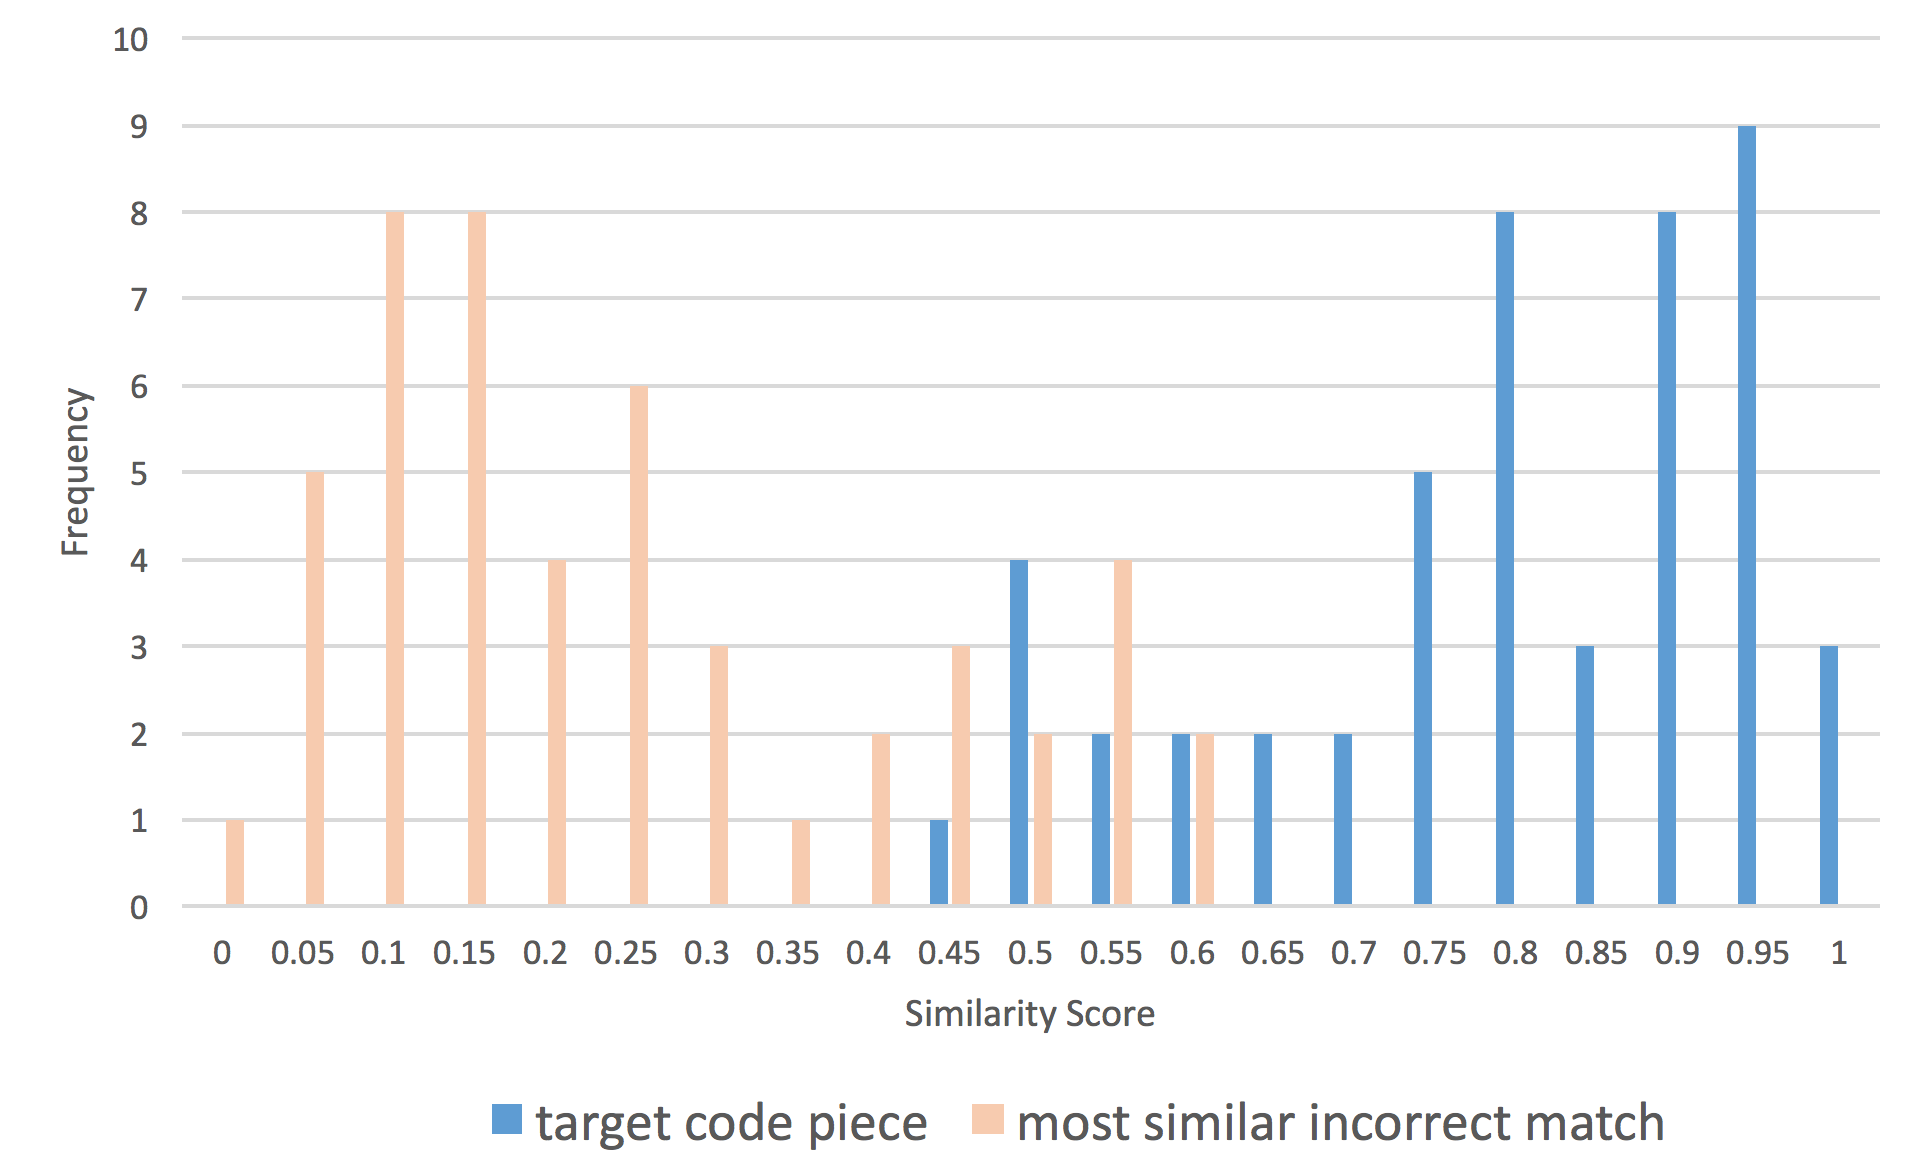
\includegraphics[width=1.0\columnwidth]{algorithm/histogram_sim.png}
%         \caption{The occurrence distributions of similarity scores of $CP_T$ (in blue) and most similar incorrect matches ($IM$, in pale orange).}~\label{fig:histogram_sim}
%     \end{figure}




% %Azoson's work
% \section{アゾソンがやったこと}
% \section{実装内容と開発背景を含む説明文の抽出手法}


\ref{section:Formative_Study}章にて述べたプログラマを対象としたインタビューにより,コード断片の理解においてプルリクエストに含まれる情報が有用であることが示唆された.
また,コード断片を理解する上で,そのコード断片が何を実行するかという実装内容だけでなく,開発背景も理解することが重要であることが明らかとなった.
しかし既存のシステムでは,コード変更の説明文に含まれる情報を,実装内容や開発背景といった情報に分類することは行われていない.
そこで我々は,プルリクエストの説明文内の文章の中から,関連するコード変更の実装方法と関連するコード変更の実装理由を抽出するための分類器を実装した.


\subsection{データセットの構築}

% \shibato{}{ExecutionとRationaleの説明が必要?}

%プルリクエストの説明文に含まれる文章をExecutionおよびRationaleに分類するためには,それらのカテゴリがラベルづけされた文章のデータセットを構築する必要がある.
%そこで我々は,GitHubのリポジトリに登録されているプルリクエストのテンプレートを活用することとした.
開発者が実装内容や開発背景といった重要な情報を漏れなくプルリクエストに記述する事を促すために,GitHubのリポジトリにはマークダウンで書かれたプルリクエストのテンプレートを登録することができる~\footnote{\url{https://help.github.com/articles/creating-a-pull-request-template-for-your-repository}}.
テンプレートに沿ってプルリクエストの説明文を記述することで,他の開発者がコード変更を理解するために必要な情報を網羅したプルリクエストを作成することができる.
テンプレート内のヘッダーには,実装内容(Execution)に該当するヘッダー(``Implementation Details''など)や,開発背景(Rationale)に該当するヘッダー(``Motivation and Context''など)などが多く採用されている.
そのようなヘッダーの下に記述されている文章を抽出することで,分類器の学習に必要なラベルづけされたデータセットを構築することとした.

以上のようなデータをGitHubから収集するために,我々は次の条件を満たすリポジトリに存在するプルリクエストのデータを抽出した.

\begin{description}
\item[条件1] リポジトリのスター数が100以上であること.
\item[条件2] プルリクエストのテンプレートがリポジトリに登録されており, Executionに関係する節かRationaleに関係する節がテンプレート内に存在すること.
\end{description}

条件1はリポジトリの開発者数の目安として掲げたものである.
スター数が大きいものほどGitHub上での開発が盛んであり,条件2を満たすプルリクエストを多く取得できるだろうと考えた.
また,条件2に適応することで,前述のようにラベルづけされたデータを収集することができる.

GitHubから条件1と条件2を満たすデータを収集した結果,26のリポジトリと4061件のプルリクエストのデータを集めることができた.
その26のリポジトリに登録されているプルリクエストのテンプレートについて,著者の2人がExecutionまたはRationaleに該当するヘッダーを手動で抽出した.
そして,それらのヘッダーの下に存在する文章を抽出することにより,Executionの文章を3141件,Rationaleの文章を3451件を得た.
さらに,抽出した文章内に含まれるマークダウン表記と絵文字を削除する事で,分類器の学習用のデータセットを構築した.


% GitHub上のリポジトリの内,以下の条件を満たすものから PR と Issue を取得し,説明文の中から上述の Why と How に関する文章を抽出することで学習用のデータセットを作成した.
% \begin{description}
% \item[条件1] リポジトリのスター数が100以上であること.
% \item[条件2] プルリクエストのテンプレートが存在し, Whyに関係する節かHowに関係する節がテンプレート内に存在すること.
% \end{description}

% 条件1はリポジトリの開発者数の目安として掲げたものである.
% スター数が大きいものほどGitHub上での開発が盛んであり,条件2を満たすプルリクエストを多く取得できるだろうと考えた.
% 条件2はプルリクエストの説明文からWhyまたはHowに該当する文章を抽出するための条件である.
% 開発者が開発目的や実装方法といった重要な情報を漏れなくプルリクエストに記述する事を支援するために,GitHubのリポジトリではマークダウンで書かれたプルリクエストのテンプレートを登録することができる~\footnote{\url{https://help.github.com/articles/creating-a-pull-request-template-for-your-repository}}.
% 開発者はテンプレートのヘッダーで指定された内容をプルリクエストの説明文に書く事で,他の開発者がコード変更を理解するために必要な情報を網羅したプルリクエストを簡単に作成できるようになる.
% 我々は収集したプルリクエストのテンプレートから,Whyに該当するヘッダー(``Motivation and Context''など)とHowに該当するヘッダー(``Implementation Details''など)を指定した.
% そして,それらのヘッダーの下に記述されている文章を,WhyおよびHowを意味する文章として抽出し,分類器の学習用のデータセットとした.

% 我々は条件1および条件2を満たす 26 のレポジトリから,4061件のプルリクエストをGitHubから収集した.
% これらの説明文の中から,Why に関係する文章を3451件,Howに関係する文章を3141件抽出した.
% そして,抽出した文章内に含まれるマークダウン表記,絵文字,urlを削除する事で,分類器の学習用のデータセットを構築した.


% \begin{table}[t]
%     \centering
%      \caption{SVMの結果}
%     \label{table:svm}
%     \begin{tabular}{c | c} \Hline
%      特徴量 &F値 \\ \hline \hline
%      bag-of-words & 0.64 \\
%      tf-idf & 0.68 \\
%      word2vec & 0.72 \\
%      word2vec+tf-idf & 0.73 \\
%     \end{tabular}
% \end{table}


\subsection{分類器の実装と評価}

分類器の実装にはサポートベクターマシンを用いた.
学習に必要な特徴量は,文章の分類において一般的に使用されているbag-of-words, tf-idf,word2vecを用いた~\cite{pmlr-v32-le14}.
さらに,tf-idfとword2vecが抽出する情報が互いに補完的な役割を果たすことが報告されているため~\cite{SVM-word2vec-tfidf},本研究においてもword2vecをtf-idfにより重み付けした特徴量(word2vec+tf-idf)も利用した.
それぞれの特徴量を用いて分類器を学習し,10分割交差検証法により分類器の精度を検証した結果,bag-of-wordsを用いた時のF値の平均が0.64,tf-idfを用いた時のF値の平均が0.68,word2vecを用いた時のF値の平均が0.72,word2vec+tf-idfを用いた時のF値の平均が0.73であった.
以上よりword2vec+tf-idfを用いた時が最も精度が高かったため,word2vec+tf-idfを用いて学習を行った分類器をCodeGlass上に実装した.

% \subsubsection{分類器によるCodeGlassの機能}


% 学習した分類器を用いることで,CodeGlassはユーザが選択したコード断片に関連するプルリクエストを,Executionの情報の量が多い順,およびRationaleの情報の量が多い順に並び替えることができる.
% ただし情報の量は,プルリクエスト内の説明文を分割し生成された各文章に対する,ExecutionまたはRationaleへの分類確率の和と定義した.
% プルリクエストの説明文の分割方法は,説明文にマークダウンが使用されていた場合,ヘッダーを区切りとして分割した.
% また,マークダウンが使用されていない説明文は,空行を区切りとして分割される.
% そして,分割された文章ごとにExecutionおよびRationaleへの分類確率を計算し,それらの和を各プルリクエストに含まれるExecutionおよびRationaleに関する情報の量とする.
% 図~\ref{fig:interface1}~(1)に示すように,CodeGlassは計算した情報の量を用いてプルリクエストを並び替えることができる.
% これによりユーザは,選択したコード断片の調査目的に合わせて,プルリクエストの表示順序を変更することができる.

% 各プルリクエストに含まれるExecutionおよびRationaleの情報の量を計算するために,CodeGlassはまずプルリクエストの説明文を分割する.
% 説明文にマークダウンが使用されていた場合,ヘッダーを区切りとして分割される.
% マークダウンが使用されていない説明文は,空行を区切りとして分割される.

図~\ref{fig:interface1}~(1)に示すボタンから,ユーザはプルリクエストの表示順を時系列順,Executionに関する情報が多い順,Rationaleに関する情報が多い順に並び替えることができる.
さらにプルリクエストの詳細画面では,ExecutionおよびRationaleに80\%以上の確率で分類されると推定された文章がハイライトされる.
図~\ref{fig:interface2}~(4)に示すように,Executionに分類される文章は緑色の,Rationaleに分類される文章は青色の文字で表示することで,ユーザの情報収集を支援することが可能となっている.





% %6
% \section{Quantitative Algorithm Evaluation}
% To evaluate the performance of our DiffTrack algorithm, we conducted two quantitative evaluations using real code revision data obtained from open source repositories on GitHub.
We have two objectives for our evaluations: 1) to quantify how accurately the algorithm can estimate a code piece; and 2) to quantify how accurately the algorithm can extract a set of commits given a code piece.
%We here report our experimental design and results.

\subsection{Code Piece Matching Accuracy}

%\subsubsection{Dataset}

\begin{table}[tbp]
	\centering
	\begin{tabular}{ c c c }
	   \small\textit{Repository Name} & \small\textit{\#Pull Requests} & \small\textit{\#Contributors} \\
       \midrule
		mailtrain & 24 & 9 \\
      portainer & 212 & 47 \\
      styletron & 32 & 9 \\
      claudia & 35 & 13 \\
      Chart.js & 1064 & 201 \\
	\end{tabular}
    \caption{Open source repositories used in our code piece matching accuracy evaluation.}
	\label{table:repositories}
\end{table}

% \begin{table}
%   \centering
%   \begin{tabular}{l r r r}
%     % \toprule
%     & & \multicolumn{2}{c}{\small{\textbf{Test Conditions}}} \\
%     \cmidrule(r){3-4}
%     {\small\textit{Name}}
%     & {\small \textit{First}}
%       & {\small \textit{Second}}
%     & {\small \textit{Final}} \\
%     \midrule
%     Marsden & 223.0 & 44 & 432,321 \\
%     Nass & 22.2 & 16 & 234,333 \\
%     Borriello & 22.9 & 11 & 93,123 \\
%     Karat & 34.9 & 2200 & 103,322 \\
%     % \bottomrule
%   \end{tabular}
%   \caption{Table captions should be placed below the table. We
%     recommend table lines be 1 point, 25\% black. Minimize use of
%     table grid lines.}~\label{tab:table1}
% \end{table}


% \begin{figure*}
%   \centering
%   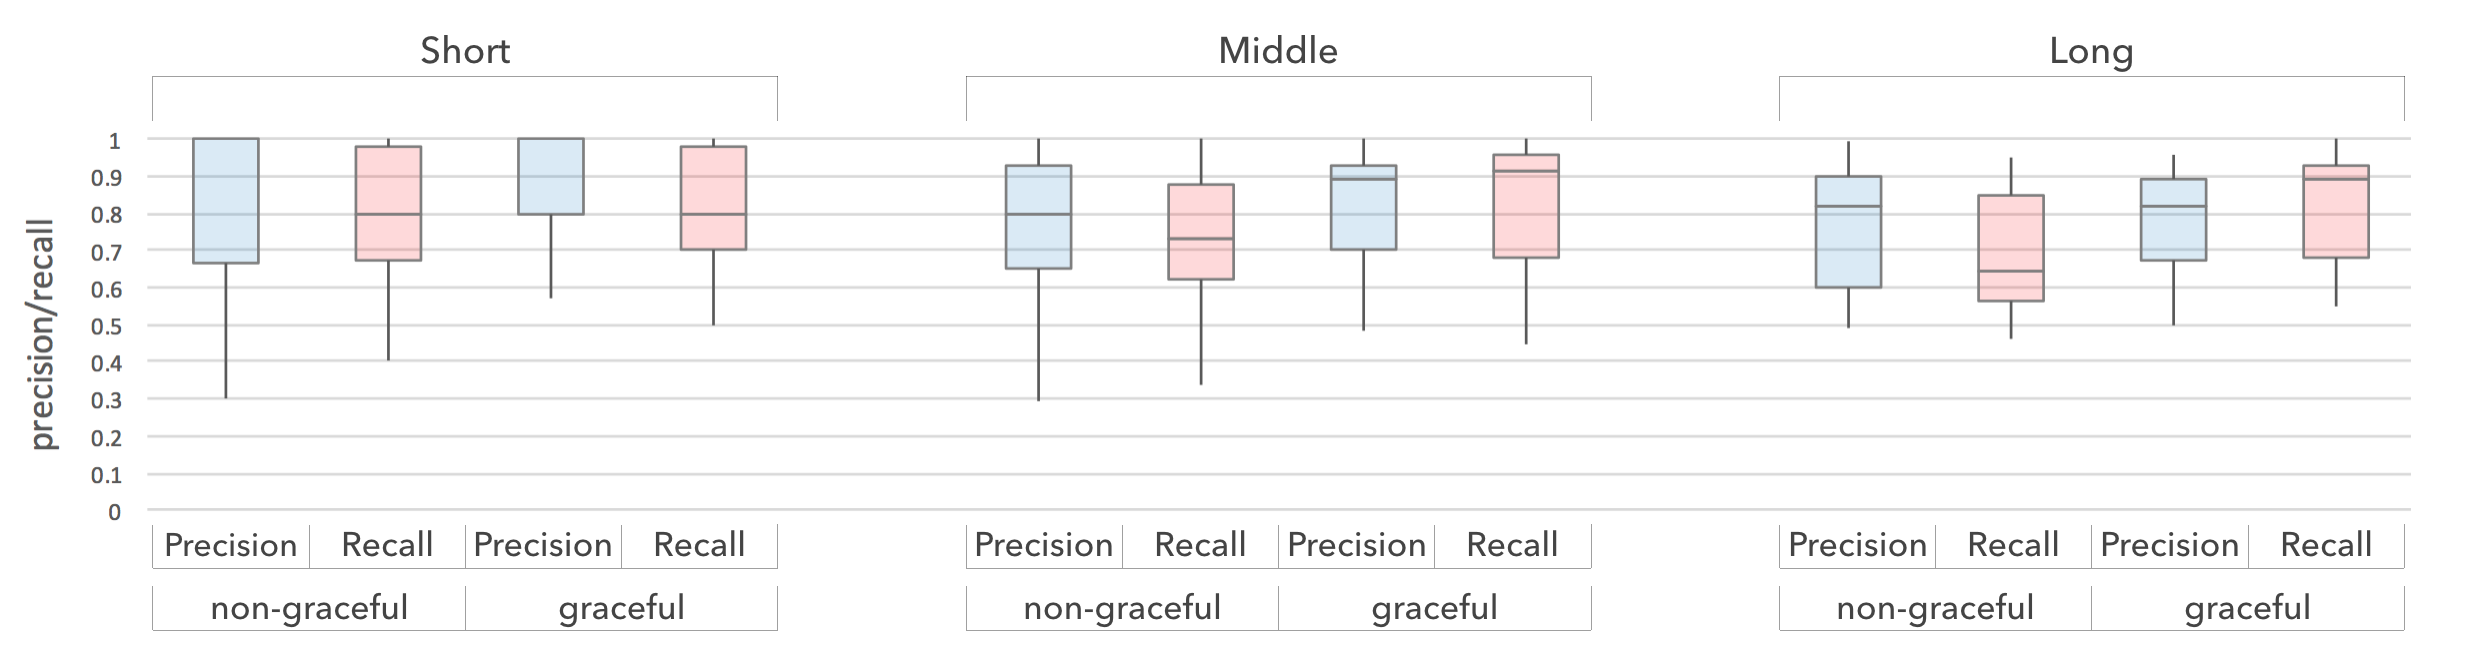
\includegraphics[width=2.0\columnwidth]{evaluate/difftrack_eval_commit.png}
%   \caption{Box plots of DiffTrack commit matching accuracy performance results.}~\label{fig:Commit_Matching_Accuracy_Evaluation}
%   \vspace{-5mm}
% \end{figure*}

We searched publicly-available repositories on GitHub that satisfied the following criteria:

\begin{itemize}
\setlength{\itemsep}{0cm}
\item A repository was active as of February 2017.
\item Multiple developers were involved.
\item Developers actively used pull requests and wrote review comments.
\item A repository was marked as favorite by over 1000 people.
\end{itemize}

As a result, we selected five repositories as summarized in Table~\ref{table:repositories}.
We then extracted commits from these repositories and manually checked them to remove minor revisions (e.g., fixing a typo) from this evaluation.
In addition, we chose commits where a knowledgeable person can easily identify a pair of code pieces between the two versions.
This process resulted in 180 commits.
After annotating ground truth data through manual labeling, we classified the collected commits into nine group (20 commits in each) in terms of the following two factors:

\begin{itemize}
\setlength{\itemsep}{0cm}
\item The types of changes included (\textit{Type}): \textit{Add} (only additions); \textit{Del} (only deletions); and \textit{AddDel} (both).
\item The number of lines changed (\textit{Length}): \textit{Short} ($\sim 9$ lines); \textit{Medium} ($10 \sim 30$ lines); and \textit{Long} ($30 \sim$ lines).
\end{itemize}

\textit{AddDel} represents cases of an update (i.e., lines in a code piece were replaced); a move (i.e., the location of a code piece was changed); a combination of both; and refactoring.
Thus, \textit{AddDel} generally represents difficult test cases for DiffTrack to accurately estimate a target code piece. 


\begin{table}[t]
    \centering
    \label{my-label}
    \begin{tabular}{cc||c|c| c}
                                                  &  & \textit{Add}           & \textit{Del}           & \textit{AddDel}        \\ \hline \hline 
\multirow{2}{*}{\textit{Short}}                     & $P_{cp}$ & 1.00 (0.00) & 0.95 (0.22) & 0.88 (0.31) \\
& $R_{cp}$ & 0.99 (0.05) & 0.95 (0.22) & 0.83 (0.32) \\ \hline
%& $F_{cp}$ & 0.99 (0.03) & 0.95 \koji{(0.95)}{} & 0.85 (0.31) \\ \hline
\multirow{2}{*}{\textit{Middle}}
& $P_{cp}$ & 0.94 (0.22) & 0.95 (0.22) & 0.96 (0.10)  \\
& $R_{cp}$ & 0.95 (0.22) & 0.95 (0.22) & 0.89 (0.15) \\ \hline
%& $F_{cp}$ & 0.95 (0.22) & 0.95 (0.22) & 0.91 (0.10)  \\ \hline
\multirow{2}{*}{\textit{Long}}
& $P_{cp}$ & 0.99 (0.06) & 0.90 (0.31) & 0.93 (0.23) \\
& $R_{cp}$ & 1.00 (0.00) & 0.90 (0.31) & 0.87 (0.23) \\
%& $F_{cp}$ & 0.99 (0.03) & 0.90 (0.31) & 0.89 (0.22)
    \end{tabular}
    \caption{Accuracy performance of code piece matching across the nine groups. $P_{cp}$ and $R_{cp}$ represent precision and recall, respectively. Values in parentheses represent the standard deviations.}
    \label{table:performance}
    \vspace{-2mm}
\end{table}




\subsubsection{Results}
Table \ref{table:performance} shows the performance of the algorithm across the nine categories.
We used the precision and recall ($P_{cp}$, $R_{cp}$) to evaluate the accuracy of estimated code pieces.
More specifically, $P_{cp} = \frac{l_c}{l_c + l_i},\;\; R_{cp} = \frac{l_c}{l_c + l_n},$ where $l_c$, $l_i$, and $l_n$ represent the numbers of lines correctly included in $\widehat{CP_{T}}$, lines incorrectly included in $\widehat{CP_{T}}$, and lines $CP_{T}$ that are not included in $\widehat{CP_{T}}$, respectively.

% \vspace{-4mm}
% \begin{equation*}
% P_{cp} = \frac{l_c}{l_c + l_i},\;\; R_{cp} = \frac{l_c}{l_c + l_n}, 
% \end{equation*}


Overall, DiffTrack exhibited high precision and recall regardless of the length of code pieces and types of revisions.
In particular, it identified code pieces almost perfectly when revisions included only additions.
Changes in \textit{AddDel} were the most difficult case, but DiffTrack was still able to identify target code pieces at reasonable precision and recall.
An evaluation on GumTree found that it was able to identify move operations accurately~\cite{GumTree} (although it is not designed to backtrack changes on code pieces as we already discussed).
Our results show that DiffTrack performs well in a wider variety of \textit{AddDel} cases, including updates, combinations of moves and updates, and refactoring.
We thus concluded that code piece matching in DiffTrack demonstrates sufficient robustness for our purpose.



\subsection{Commit Matching Accuracy Evaluation}
%\subsubsection{Dataset}
We evaluated the accuracy of selected commits by DiffTrack.
We chose  100 code pieces (34 \textit{Short}, 33 \textit{Middle}, and 33 \textit{Long}) from the Chart.js repository.
We then manually traced back the development history, and created the ground truth data consisting of more than five commits associated with each original source code piece.


\subsubsection{Results}
We used precision and recall for this evaluation.
The definitions of these metrics are the same as those for the code piece matching performance evaluation except using the number of commits.
Figure~\ref{fig:Commit_Matching_Accuracy_Evaluation} shows the performance of the algorithm.
Overall accuracy performance was high regardless across the conditions.
We ran multi-level linear regression analysis with two factors: \textit{Length} and the presence of graceful matching.
The result showed that graceful matching significantly improved precision and recall.
The estimated coefficients were 0.058 ($SE=0.025$, $p<0.05$) and 0.051 ($SE=0.021$, $p<0.05$) for precision and recall, respectively.
\textit{Short} also showed significantly higher precision and recall than \textit{Long} ($p<0.05$).


The results suggest that our graceful approach can improve precision and recall of identifying commits by roughly 5\% in our dataset.
Although the effect estimated by our multi-level linear regression was not large, it offers robustness to cases in which the default DiffTrack algorithm exhibits low precision and recall as shown in Figure~\ref{fig:Commit_Matching_Accuracy_Evaluation}.
In one test case, the na\"{i}ve DiffTrack algorithm was only able to achieve the precision and recall of 0.30 and 0.40, respectively, but the graceful approach improved both of them to 0.80.
We thus concluded that the graceful approach can improve commit matching and should be included in the CodeGlass system.



% %7
% \section{Quantitative User Evaluation}
% Our algorithm evaluation confirms that DiffTrack can robustly trace changes on code pieces.
We thus conducted a quantitative study to investigate how well the CodeGlass interface can support comprehension of code pieces. 

\begin{table*}[t]
    \centering
    \begin{tabular}{c||ccc|ccc}
    \multirow{2}{*}{Category} & \multicolumn{3}{c|}{\textbf{without CodeGlass}} & \multicolumn{3}{c}{\textbf{with CodeGlass}} \\
     & Precision & Recall & Confidence & Precision & Recall & Confidence \\ \hline \hline
     Execution & 0.77 (0.12) & 0.46 (0.08) & 74.5 (9.67) & 0.80 (0.18) & 0.49 (0.13) & 79.5 (7.14) \\
     Rationale & 0.54 (0.38) & 0.14 (0.09) & 63.9 (28.1) & 0.79 (0.21) & 0.29 (0.06) & 78.3 (11.6) \\
     History & 0.35 (0.35) & 0.08 (0.02) & 8.6 (17.7) & 0.88 (0.13) & 0.16 (0.01) & 66.6 (6.25) \\ 
    \end{tabular}
    \caption{Accuracy performance and confidence scores in the user evaluation. Values in parentheses represent the standard deviations.}
    \label{table:experiment_result}
    \vspace{-2mm}
\end{table*}

\begin{table}[t]
    \centering
    \begin{tabular}{rl||ccc}
    \multicolumn{2}{l||}{Metric} & $t(7)$ & $p$ & Cohen's $d$ and 95\%CI \\ \hline \hline
    \multicolumn{2}{l||}{\textbf{Execution}} & & & \\
    & Precision & 0.76 & \textit{n.s.}%0.47
    & 0.27 [-0.44, 0.97] \\
    & Recall & 0.74 & \textit{n.s.}%0.48 
    & 0.26 [-0.45, 0.96] \\
    & Confidence & 1.77 & \textit{n.s.}%0.12 
    & 0.63 [-0.16, 1.37] \\ \hline
    \multicolumn{2}{l||}{\textbf{Rationale}} & & & \\
    & Precision & 1.79 & \textit{n.s.}%0.12 
    & 0.63 [-0.15, 1.38] \\
    & Recall & 3.55 & < 0.01 & 1.25 [0.28, 2.18] \\
    & Confidence & 1.57 & \textit{n.s.}%0.16 
    & 0.55 [-0.21, 1.29]\\ \hline
    \multicolumn{2}{l||}{\textbf{History}} & & & \\
    & Precision & 4.58 & < 0.01 & 1.62 [0.52, 2.68] \\
    & Recall & 5.97 & < 0.001 & 2.11 [0.81, 3.38] \\
    & Confidence & 5.41 & < 0.001 & 1.91 [0.69, 3.09] \\ 
    \end{tabular}
    \caption{Paired t tests on user evaluation performance results.}
    \label{table:stats_result}
    \vspace{-2mm}
\end{table}


\subsection{Experimental Design}

\subsubsection{Hypothesis}
Our literature survey identified the following five information categories developers seek in code comprehension:

\begin{itemize}
\setlength{\itemsep}{0cm}
\item \textbf{Execution}: What the given code piece executes~\cite{Information_Needs_in_Collocated_Software_Development_Teams}.
\item \textbf{Rationale}: Why the given code piece is implemented in the way it is~\cite{Information_Needs_in_Collocated_Software_Development_Teams}.
\item \textbf{History}: How the given code piece has been evolved~\cite{Chronicler}.
\item \textbf{Contributor}: Who was involved in the implementation of the given code piece~\cite{Who_can_help_me_with_this_source_code_change}.
\item \textbf{Usage}: Where and how the given code piece is used in a project~\cite{Six_Learning_Barriers_in_End_User_Programming_Systems}.
\end{itemize}

We found that existing tools support Contributor and Usage information seeking (e.g., git-blame to identify who made a particular change).
Therefore, we decided to mainly examine the user performance of finding information for \textbf{Execution}, \textbf{Rationale}, and \textbf{History} in our evaluation.
These information categories were also found important by the professional developers in our interview study.

% We then developed the following hypotheses to derive our experimental design:

% \begin{itemize}
% \setlength{\leftskip}{4mm}
% \setlength{\itemsep}{0mm}
% \item[H1.] \textit{CodeGlass would not degrade accurate and precise execution understanding for code pieces.} This is because that CodeGlass does not prevent participants from examining raw code.  
% \item[H2.] \textit{CodeGlass would support more accurate and precise rationale understanding for code pieces.} This is because that past pull requests in CodeGlass can contain information about why code changes were made.  
% \item[H3.] \textit{CodeGlass would support more accurate and precise understanding of development history for code pieces.} This is because that a series of relevant past pull requests in CodeGlass can suggest the evolution of code pieces.
% \end{itemize}



\subsubsection{Task}
Debugging is a common task to assess the effect of code comprehension tools \cite{Code_Bubbles,Improving_API_Documentation_Usability_with_Knowledge_Pushing}.
In such a task, participants are asked to identify and fix intentionally-introduced bugs.
However, our system involves version control, and thus participants would be able to easily identify what changes would be needed to complete a task.



Instead, we decided to employ short documentation creation tasks.
We provided a simple text format for documenting execution, rationale, and history information.
Participants were asked to itemize any important information in these categories about the given code piece.
For each item, they also provided their confidence score from 0 to 100 in order to indicate how confident they were that the description was correct.
A higher score means a description with stronger confidence.
To avoid making our experiment unnecessarily long, we set the time limit for each task to 20 minutes.

We created four tasks using the repository of Chart.js in this experiment.
Two of the authors jointly examined the repository and developed information items that both agreed were important enough to be documented.
The tasks had 10.8, 9.8, and 7.3 items on average as answer keys for execution, rationale, and history categories, respectively.
Each task used a code piece from a different source code in Chart.js to avoid learning effects.
We chose the following files under the same directory: core.animation.js, core.canvasHelpers.js, core.ticks.js, and core.title.js\footnote{Note that this was moved to plugin.title.js as of March 26, 2017.}. 


\subsubsection{Procedure}
The participants were asked to come to our laboratory for this study.
After they signed a consent form, we explained the CodeGlass interface and tasks.
When the participants felt comfortable with the tasks and CodeGlass, we started the experiment.
We had four tasks in total (Task A, B, C, and D) and two conditions: the GitHub Web interface with the presence and absence of CodeGlass (CG and non-CG).
The two sets of tasks were counter-balanced for the two interface conditions across participants.
We fixed the order of the tasks in each set.
We alternatively switched the interface conditions with always starting with the reference condition.
Thus, the order for the half of our participants was Task A/non-CG; Task B/C
G; Task C/non-CG; and Task D/CG. 
The rest of the participants were exposed to Task B/non-CG first, followed by Task A/CG; Task D/non-CG; and Task C/CG. 
As all of our participants had sufficient experience on GitHub, we expected that starting with the non-CG condition would not cause undesirable learning effects.

After the participants completed all four tasks, we conducted a short semi-structured interview to understand their subjective impressions about CodeGlass and its potential use.
The participants were offered a compensation of approximately 15 USD cash in a local currency.

\subsubsection{Participants}

As our tasks involve code comprehension, we set several criteria for participants: 1) their programming experience should be longer than one year; 2) they should be familiar with GitHub; 3) they should be knowledgeable in JavaScript; and 4) they were not involved in the Chart.js project.
Our participants would thus represent developers who have enough knowledge and experience on reading code but do not own the background about a project.
Our selection criteria also reflected one of our target use cases of CodeGlass: junior developers who join a new team now need to acquire understanding of source code in a project to engage in various tasks.
We mainly recruited participants from our institute.
As a result, 8 people volunteered (PC1--8; all male; 22.1 years old on average).

 

\subsection{Results}


%\subsubsection{Quantitative Results}
We counted how many points in our answer keys documentation created by our participants covered.
We then calculated the precision and recall based on the number of correct items similar to the evaluations above.
When there was no documented item for a particular category, we regarded all evaluation metrics as 0.
Table~\ref{table:experiment_result} shows the means and standard deviations of the precision, recall, and confidence scores.
The precision values in the CodeGlass condition were high for all documentation categories.
The recall values for rationale and history documentation had improvements with CodeGlass.
Table~\ref{table:stats_result} summarizes results of paired t tests.
We found significant differences for recall and all scores in rationale and history documentation, respectively.

%\subsubsection{Subjective feedback}
During the post-experimental interviews, our participants expressed various potential use of CodeGlass: understanding unfamiliar code (7 participants); learning how to fix bugs (3 participants); and self-training with open source projects (2 participants).
Four participants explicitly mentioned that the response speed of CodeGlass was fast enough for their interaction.

% \subsubsection{Comments from Participants}
% % Four of our participants (P2, P3, P6, and P7) explicitly mentioned that the response speed of CodeGlass was fast enough for their interaction.
% % The rest of the participants did not complain its responsiveness, and we thus concluded that CodeGlass was well implemented for practical use.

% Participants mentioned several interesting use scenarios of CodeGlass.
% P5 commented that CodeGlass could help him understand part of code which he is not familiar with.
% This is in line with our main target use scenario informed through interviews with professional developers.

 % %P5: 自分が使いたいと思うときっていうのはやっぱり複数人でやってるんだったら自分が担当してない部分のコードを理解したいなーって思うときにこれを。
% \myquote{I want to use this (CodeGlass) when I work in a team and want to understand a part of code which I am not in charge of.}{PB5}

% PB3 shared his view with us that development history information provided by CodeGlass could inform how to fix and even avoid possible bugs.
% %P3: むしろこれはなんか、プログラム中級者がさ、開発歴見てああ俺もこういうバグやっちまうわーみたいなので共感して、ああこう治すんだっていう知識を仕入れるときに良さそう。
% \myquote{I think this (CodeGlass) is useful when intermediate-level programmers can look at development history and see `Ah, I would do the same mistake.' Then they can learn how to fix such bugs.}{PB3}

% We also asked our participants how they would use CodeGlass for open source projects.
% Two participants (PB5 and PB7) responded that CodeGlass can help self-learning.
% PB7 commented that he could exploit open source projects much more than the default GitHub interface for his self-learning.
% %P5: オープンソースでやるなら、そうだな自分も全然ただの開発に携われるようなスキルを持ってるわけじゃないから直接連絡とかは取れないしって思うんだったら全然これを使って勉強するっていうか、理解するのはやっぱり無いよりかは分かりやすかったと僕は思いました。}
% %\myquote{Well, I do not have enough skills to get involved in (open source) projects. So I am hesitant to directly contacting contributors. But if I can use this (CodeGlass), I can learn code by myself.}{PB5}
% %P7: だから、どんどん新しいそのなんでも教材に出来るっていうか。どんなそのGitHubのものも、例えば先生を見つけてくれば、簡単なものから複雑なものまで、全部どういうコードでこの人が書いたかっていうのが、今まではソースとかコメントしか読めなかったけども、プロジェクト自体がどうやって運んでいくかっていうのもちょっと引いた目で見るみたいなことがいろいろな教材も無限にあるし、っていうのでいいんじゃないかなと。
% \myquote{I can use anything as a learning material. If I can find a good example, regardless of simple or complex code, I can see how developers wrote code. Until now, I can only read source code and comments. But [with CodeGlass] I can have a higher-level view on how the project is going on.}{PB7}


% %8
% \section{Discussion}
% As we already discussed the algorithm evaluation results before, we here mainly examines results in our user study.
The quantitative results confirm that CodeGlass fully outperformed in history understanding.
Our user evaluation showed that CodeGlass significantly improves the recall of implementation rationale understanding, but not precision.
One possible reason was that implementation rationales can be inferred to some extent if execution was well understood.
As a result, the reference condition might have shown comparable precision results.
Because we observed a difference in recall, we conclude that our CodeGlass showed partial outperformance in rationale understanding.

Recall was rather low across the conditions.
One possible explanation was that our user study had time limits to make the evaluation tractable.
But, our results are still positive because participants were able to develop precise understanding in all three information categories with CodeGlass.

The confidence scores showed differences in the history understanding.
93.5\% and 90.8\% of the documented items by participants had confidence scores of 50 and above in the reference and CodeGlass condition, respectively.
This suggests that the participants tended to document only items on which they had a certain level of confidence.
The confidence scores for history understanding in the reference condition was an exception because many participants simply failed to identify any item in the reference condition.
This result also confirms the advantages of CodeGlass.


% %9
% \section{Informal Expert Review}
% Our user evaluation with novice developers (i.e., university students) confirms the benefits of CodeGlass.
To validate the potential of our system for professional use, we conducted informal expert reviews.
We recruited 8 expert programmers (PD1--PD8, all male) in 4 different IT companies.
Our interviewees agreed on benefits of CodeGlass the lab study participants also mentioned: support examining past pull requests (8 participants); facilitate developer onboarding (5 participants); and comprehend open source code (4 participants).
Beside these benefits, they expressed potential advantages for professional use.

\subsection*{Understanding Hidden Development Context}

In real development environment, programmers do not always achieve the most efficient coding due to various reasons (e.g., tight deadlines and lack of coding skills).
Raw code does not necessarily offer such backgrounds when developers revisited.
PD3 and PD7 stated that CodeGlass can help them obtain such past backgrounds of source code.

% \myquote{昔のリポジトリのメンテナンスとかしてると結構危ないコードがあって、でも当時のチーム構成や技術力だったりリリースしないといけないみたいなのを考えると仕方なかったりするんですよね。そういうのを過去のログ(プルリク)から読み取れていい。}{P3}

%\myquote{When I am taking care of old repositories, I often find pretty dangerous code. But it could not be helped because we didn't have enough team members and skills at that time. This [CodeGlass] can help me view such background stories from past logs, and I like it.}{PD3}

% \myquote{新規で入ってコード見ると、だめなコードがたくさんあるんですよね。でも実はそれは特定の技術を使ってはいけないみたいな制約のもとの苦渋の決断だったことってかなりあるんですよね。そういうのはコードをみても絶対に分からないし、かといって大規模だと履歴を追うのは相当つらい}{P7}

\myquote{Horribly-written code is often a product of tough decisions by various constraints. Such backgrounds would never be visible from code, but it is tedious to review histories in a large-scale project.}{PD3}

Although projects have specifications, they were changed over code revisions.
As a result, such specifications do not offer correct information about existing code.
Pull requests extracted by CodeGlass would be useful to fill the discrepancy between outdated specifications and code.

% \myquote{コードが仕様と合わなくなったり逆に仕様書とか読んだら間違ったりとかあるので、コードが一番大事というか、正確で、ただそのコードがなぜ入ったかっていうのは昔のプルリクエストで見るんで、そういう時に使えると思います。}{P3}

% \myquote{こういう大きい会社ではいろんな人がすごいスピードで開発しててドキュメントもないから、全体的なコード理解にはすごくいいと思う。}{P6}

% \myquote{仕様書をもとにコードを作って、仕様書をもとにテストするんですが、でもやっぱり経緯はわかんないし、仕様書とコードの間のギャップって凄まじいんですよね。仕様書もコードも結果であって、開発理由とかは本当にわからない}{P7}

\myquote{We write and test code based on a specification. But it doesn't tell me how the code has been developed. And a gap between the specification and actual code is huge. Both specifications and code are just end products, and they don't tell me reasons why they are here.}{PD7}


\subsection*{Documentation through Pull Requests}

Although the importance of software documentation is well known, developers do not spare time and effort for it in reality~\cite{A_Study_of_the_Documentation_Essential_to_Software_Maintenance}.
%The participants also stated that they do not create detailed documentation, and pull requests can be a useful information resource to understand the rationale of source code.
PD5 and PD8 shared with us a unique idea that CodeGlass could encourage them to write detailed pull requests for future revisitation.

% \myquote{これ見て思ったのは、後からプルリクを分かりやすいように書き直したいと思うだろうなと思って、情報をどんどんあとから追加してWikiとかドキュメントみたいにできるかも。}{P5}

% \myquote{ソースコードのドキュメントって最近廃れてきてる気がしていて、よく関数名の上にコメント書くとドキュメントができたり、変数名からドキュメント作るやつありますけど、結局面倒とかqualityが低いとか、あと情報量がないので使わないんですよね。何してるかなんてある程度コード見たらわかるのでどうでもよくて、やっぱりなぜそのコードになったのかが重要で、プルリクは開発フローに既にあるし、それをもう少しちゃんと書いたらドキュメントになるってのはすごく新しいし実用的ですね}{P8}


\myquote{It's important to share why we wrote this particular code. Because pull requests are already in our development process, and (with CodeGlass) if we write them a little more properly, they become documentations. That's pretty new and practical.}{P8}

% \subsection*{Assisting to Understand Codes in Open Source Projects}

% CodeGlass works on all repositories on GitHub by only cloning them to the server system.
% Developers often investigate open source projects to understand external libraries they use in their projects.
% They also see open source as a means of learning good coding practices.
% CodeGlass has a great potential for supporting code understanding in open source projects by using such resources.
% The participants agree on this as a potential use of CodeGlass.

% \myquote{僕がオープンソースを読むのは、一個はちょっと参考になるとか勉強しようとか、なんかメジャーなリポジトリがどう作られてるかとか勉強目的で読むのと、あとはうちが使ってるライブラリとかあるんですよね、で、それらが挙動がよくわかんない時とか、より深く見ていきたい時とかっていうのは、なんでこういう実装というか、意図はなんなんだみたいな、深く見る時に使うかなあと思います。}{P1}


% \myquote{オープンソースだったらめっちゃ喜ばれそうですねえ、僕らは大体使ってるライブラリに何か問題があった時に、見に行ったりするので、めっちゃ助かりますね。}{P4}


\subsection*{Supporting Code Review}

Code review is a common practice in professional development environment for quality control.
But proper code review requires deep comprehension of revisions and their reasons.
%Reviewers also have to acquire the context and history of the project to fully understand the changes.
3 participants mentioned that CodeGlass would be helpful in code review because it offers quick access to relevant past pull requests.

% \myquote{レビューしていてコードの意図がわかんない時とか、かなり複雑なコードだった時に、プルリクに詳しく説明があるかなあって感じだったので、今言ったような時に使うかなあと}{P1}

\myquote{When I don't understand the intention of the given code or when it is very complex, I expect there may be some details in pull requests, so it [CodeGlass] could be useful for that.}{PD1}

% \myquote{これを使えばプルリクの履歴でまあそれを探し出せる、もちろんレビューの時に情報は多いほうがいいので。}{P3}
%\myquote{With this [CodeGlass], I can find (information about context) from past pull requests. It's always good to have as much information as possible when I do code review.}{PD3}

% \myquote{レビューしててそもそもこのクラス全体は何用だっけとかなるので、レビュー中は特に大雑把にコードの意味を思い出したいことがたしかに結構ある。}{P6}





% % Conclusion
% \section{Limitations}
Although our results suggest a strong potential of CodeGlass and DiffTrack, there are several limitations in our study.
An evaluation with a larger dataset is necessary to investigate the true performance of DiffTrack.
The current DiffTrack implementation generally takes a couple of seconds to identify code pieces in past pull requests.
Our lab study participants did not mention noticeable delays by the system.
Algorithm optimization and speed performance evaluations are out of our main scope though they are important future work.
%Future work should investigate how to optimize its process.

CodeGlass would not be effective if a project does not regularly use pull requests or developers do not write proper descriptions in commits.
Prior work has investigated a tool to support developers to write commit descriptions~\cite{ChangeScribe}, which can co-exist with CodeGlass.
Because information provided through CodeGlass is useful for code comprehension, our system could also encourage a practice of using pull requests and writing detailed comments from a different perspective. 

DiffTrack does not currently support backtracking at a word- or character-level of granularity.
Such a capability would enable new use scenarios (e.g., looking into the implementation history and reasons for a particular variable).
However, very accurate syntactic understanding would be necessary.
Future work should investigate how AST-based methods~\cite{GumTree, Change_Distilling} could support finer-level code examination.

\section{Conclusion}

We presented CodeGlass, an interface that provides pull requests and their review comments associated with a code piece.
%We also developed a piece-level diff backtrack algorithm, called DiffTrack.
Given a code piece, our DiffTrack algorithm identifies its location in an older version even if changes were made.
It precisely and accurately extracts a series of commits that include changes on the chosen code piece.
CodeGlass then shows a series of pull requests containing these commits for supporting user's comprehension.
Our quantitative evaluation on the DiffTrack algorithm shows high precision and recall results for various types of revisions.
In addition, our user study confirmed that CodeGlass was most useful to obtain development rationale and history about code pieces.
Expert reviews confirmed potential advantages of CodeGlass in professional use.


% References
\bibliographystyle{ipsjsort}
\bibliography{ref}

\end{document}
